\documentclass[oldfontcommands, a4paper, 12pt]{memoir}%\stockbv\pageaiv

\usepackage[T1]{fontenc}
\usepackage[utf8]{inputenc}
\usepackage[a4paper]{geometry}%[b5paper]{geometry}%[a4paper]{geometry}
\geometry{verbose,tmargin=2.5cm,bmargin=2.5cm,lmargin=2.5cm,rmargin=2.5cm}
%\usepackage{geometry}
%\geometry{
% b5paper
% total={170mm,257mm},
% left=20mm,
% top=20mm,
% } 
\pagestyle{Ruled}
%\settypeblocksize{6.5in}{4.5in}{*}
%\setlrmargins{*}{*}{1}
%\checkandfixthelayout
\usepackage{array}
\usepackage{verbatim}
\usepackage{prettyref}
\usepackage{booktabs}
\usepackage{textcomp}
\usepackage{url}
\usepackage{amsmath}
\usepackage{chemarr}%flechas para reacciones químicas (SFER.tex)
\usepackage{graphicx}
\usepackage{amssymb}
\usepackage{nomencl}
\usepackage[usenames,dvipsnames]{xcolor}
%\usepackage{subfig}
\usepackage{subcaption}


\newcommand\blfootnote[1]{%
  \begingroup
  \renewcommand\thefootnote{}\footnote{#1}%
  \addtocounter{footnote}{-1}%
  \endgroup
}

\newcommand{\starbreak}{%
    \fancybreak{* * *}%
}

%\includeonly{Discusion}

\OnehalfSpacing
 
% the following is useful when we have the old nomencl.sty package
%\providecommand{\printnomenclature}{\printglossary}
%\providecommand{\makenomenclature}{\makeglossary}

%\makenomenclature

\usepackage[caption=false]{subfig}
%Configuración de los caption
%\PassOptionsToPackage{caption=false}{subfig}%Evita que el paquete subfig lo descabale todo
\captiontitlefont{\itshape}
\captionnamefont{\scshape}
\captionsetup{font=footnotesize}
%\captionstyle{\centering}
\hangcaption


%\usepackage[spanish]{babel}
%\addto\shorthandsspanish{\spanishdeactivate{~<>}}
 

\usepackage[emulate=units]{siunitx}
\sisetup{per=fraction, fraction=nice}
\newunit{\wattpeak}{Wp}
\newunit{\watthour}{Wh}
\newunit{\watt}{W}
\newunit{\metro}{m}

% \usepackage{lscape}
\usepackage{mathpazo}%Letra palatino con fuentes para matemáticas
\usepackage{flafter}%obliga a que los flotantes aparezcan después de su referencia
\usepackage{memhfixc}
\usepackage{mempatch}


\raggedbottom
\sloppybottom
\clubpenalty=10000
\widowpenalty=10000

%\raggedbottomsection
\feetbelowfloat

% !! esta seccion esta comentada en veleta

\usepackage[citestyle=alphabetic, bibstyle=alphabetic, maxbibnames=5, minbibnames=3, backend=bibtex, doi=true, url=true]{biblatex}

% \DefineBibliographyStrings{spanish}{%
%   andothers        = {et\addabbrvspace al\adddot},
%   andmore          = {et\addabbrvspace al\adddot},
%   in               = {},
% }

\DefineBibliographyStrings{English}{
  andothers        = {et\addabbrvspace al\adddot},
  andmore          = {et\addabbrvspace al\adddot},
  in               = {},
}


% \addbibresource{../biblio.bib}
\addbibresource{Data5.bib}

\let\cite\parencite

\renewcommand{\bibsection}{%
	\chapter*{\bibname}
	\bibmark
	\phantomsection
	\addcontentsline{toc}{chapter}{\bibname}
	\prebibhook}
\renewcommand{\bbltechreport}{Informe T\'ecnico}

% !!

%definition of some colors I could use.      
\definecolor{amaranth}{rgb}{0.9, 0.17, 0.31}
\definecolor{brightmaroon}{rgb}{0.76, 0.13, 0.28}

\usepackage{hyperref}


\hypersetup{
    bookmarks=true,         % show bookmarks bar?
    unicode=true,          % non-Latin characters in Acrobat’s bookmarks
    bookmarksnumbered=false,
    bookmarksopen=false,
    breaklinks=true,
    backref=true,
    pdftoolbar=true,        % show Acrobat’s toolbar?
    pdfmenubar=true,        % show Acrobat’s menu?
    pdffitwindow=false,     % window fit to page when opened
    pdfstartview={FitH},    % fits the width of the page to the window
    pdftitle={Tesis Claudia},    % title
    pdfauthor={Claudia Gutiérrez},     % author
    pdfsubject={Energia Solar Fotovoltaica},   % subject of the document
    pdfcreator={AucTeX/Emacs},   % creator of the document
    pdfproducer={LaTeX}, % producer of the document
    pdfkeywords={radiación solar, energía solar fotovoltaica, energías
    renovables}, % list of keywords
    pdfnewwindow=true,      % links in new window
    pdfborder={0 0 0},
    colorlinks=true,       % false: boxed links; true: colored links
    linkcolor=grey,          % color of internal links
    citecolor=brigthmaroon %BrickRed,        % color of links to bibliography
    filecolor=black,      % color of file links
    urlcolor=Blue           % color of external links 
}
	

\DeclareSIUnit\kWh{kWh}
\DeclareSIUnit\Wh{Wh}
\DeclareSIUnit\Wp{Wp}
\DeclareSIUnit\kWp{kWp}
\DeclareSIUnit\amperehour{Ah}
\DeclareSIUnit\celula{celula}

%\spanishdecimal{.} %Para que no lo sustituya automáticamente por comas
\addto\captionsspanish{%
\def\tablename{Tabla}%
\def\listtablename{\'Indice de tablas}}

\renewcommand\nomname{Nomenclature}
\def\nompreamble{\addcontentsline{toc}{chapter}{\nomname}\markboth{\nomname}{\nomname}}


%\@addtoreset{equation}{section}
%\renewcommand{\theequation}{\thesection.\arabic{equation}}
%\numberwithin{equation}{section}
%\@addtoreset{table}{section}
%\renewcommand{\thetable}{\thesection.\arabic{table}}
%\numberwithin{table}{section}
%\@addtoreset{figure}{section}
%\renewcommand{\thefigure}{\thesection.\arabic{figure}}
%\numberwithin{figure}{section}


%\declarebtxcommands{spanish}{%
 % \def\btxphdthesis#1{\protect\foreignlanguage{spanish}{Tesis Doctoral}}%
%}
%\setbibliographyfont{lastname}{\scshape}%Pone los autores en Small Caps



%Configuración de MEMOIR
%%Pone la fecha en SMALL CAPS y hacia la derecha
%%pagina 60 de memman.pdf
\pretitle{\vfill \begin{center} \bfseries\HUGE \color{Black}}% \scshape \HUGE \color{Black}}
\posttitle{\par\end{flushright}}

\preauthor{\begin{center} \large}% \scshape}
\postauthor{\par\end{flushright}}

\date{}
\predate{\vfill \begin{flushright}\large\scshape}
\postdate{\par\end{flushright}\vfill}

\setsecnumdepth{subsection}


%\definecolor{ared}{rgb}{.647,.129,.149}
%\renewcommand{\colorchapnum}{\color{ared}}
%\renewcommand{\colorchaptitle}{\color{ared}}
%\chapterstyle{pedersen}
\chapterstyle{ger}

\setlength{\afterchapskip}{35pt}
\maxtocdepth{section}

% \setcounter{topnumber}{3}
%\setcounter{bottomnumber}{2}
%\setcounter{totalnumber}{4}
\renewcommand{\topfraction}{0.85}%{0.85}
\renewcommand{\bottomfraction}{0.5}
\renewcommand{\textfraction}{0.15}
\renewcommand{\floatpagefraction}{0.7}


%Centra las figuras en los flotantes y los enmarca
\makeatletter
\renewenvironment{figure}[1][]{%
     	\@float{figure}%
		%\begin{framed}    
		%\precaption{\rule{\linewidth}{0.4pt}\par}%En las figuras el caption va debajo
		%\hrule\vspace{0.5\onelineskip}
		\centering
		  }{%
		%\end{framed}
		\postcaption{\rule{\linewidth}{0.4pt}}
		\vspace{1.5\onelineskip}\hrule
    	\end@float	
}
\makeatother

\makeatletter
\renewenvironment{table}[1][]{%
      	\@float{table}%
		%\begin{framed}    
		\postcaption{\rule{\linewidth}{0.4pt}\par}%En las tablas el caption va encima
		\centering
		  }{%
		%\end{framed}
    	\end@float	
}
\makeatother


\renewcommand{\textfloatsep}{20pt}%Espacio entre el flotante y el texto

%backgroung image
\usepackage{eso-pic} 

%http://stackoverflow.com/questions/240097/how-to-create-a-background-image-on-titlepage-with-latex
\newcommand\BackgroundPic{
  \put(350,-150){
    \parbox[b][0.5\paperheight]{0.5\paperwidth}{%
      \includegraphics[scale=0.5]{../figs/johnny_automatic_old_sun}%
}}}

\newcommand\BackgroundPicLight{
  \put(350,-150){
    \parbox[b][0.5\paperheight]{0.5\paperwidth}{%
 %     \vfill 
%\centering
      \includegraphics[scale=0.5]{../figs/johnny_automatic_old_sun_light}%
%\vfill
}}}

%claudia

\renewenvironment{abstract}%
{\cleardoublepage\null \vfill\begin{center}%
    \bfseries\abstractname\end{center}}%
{\vfill\null}

%%%% claudia:
% \usepackage{color,calc,graphicx,soul,fourier}
% \definecolor{nicered}{rgb}{.647,.129,.149}
% \makeatletter
% \newlength\dlf@normtxtw
% \setlength\dlf@normtxtw{\textwidth}
% \def\myhelvetfont{\def\sfdefault{mdput}}
% \newsavebox{\feline@chapter}
% \newcommand\feline@chapter@marker[1][4cm]{%
% \sbox\feline@chapter{%
% \resizebox{!}{#1}{\fboxsep=1pt%
% \colorbox{nicered}{\color{white}\bfseries\sffamily\thechapter}%
% }}%
% \rotatebox{90}{%
% \resizebox{%
% \heightof{\usebox{\feline@chapter}}+\depthof{\usebox{\feline@chapter}}}%
% {!}{\scshape\so\@chapapp}}\quad%
% \raisebox{\depthof{\usebox{\feline@chapter}}}{\usebox{\feline@chapter}}%
% }
% \newcommand\feline@chm[1][4cm]{%
% \sbox\feline@chapter{\feline@chapter@marker[#1]}%
% \makebox[0pt][l]{% aka \rlap
% \makebox[1cm][r]{\usebox\feline@chapter}%
% }}
% \makechapterstyle{daleif1}{
% \renewcommand\chapnamefont{\normalfont\Large\scshape\raggedleft\so}
% \renewcommand\chaptitlefont{\normalfont\huge\bfseries\scshape\color{nicered}}
% \renewcommand\chapternamenum{}
% \renewcommand\printchaptername{}
% \renewcommand\printchapternum{\null\hfill\feline@chm[2.5cm]\par}
% \renewcommand\afterchapternum{\par\vskip\midchapskip}
% \renewcommand\printchaptertitle[1]{\chaptitlefont\raggedleft ##1\par}
% }
% \makeatother
% \chapterstyle{daleif1}
%probar bluebox

% \usepackage{calc,color}
% \newif\ifNoChapNumber
% \newcommand\Vlines{%
% \def\VL{\rule[-2cm]{1pt}{5cm}\hspace{1mm}\relax}
% \VL\VL\VL\VL\VL\VL\VL}
% \makeatletter
% \setlength\midchapskip{0pt}
% \makechapterstyle{VZ43}{
% \renewcommand\chapternamenum{}
% \renewcommand\printchaptername{}
% \renewcommand\printchapternum{}
% \renewcommand\chapnumfont{\Huge\bfseries\centering}
% \renewcommand\chaptitlefont{\Huge\bfseries\raggedright}
% \renewcommand\printchaptertitle[1]{%
% \Vlines\hspace*{-2em}%
% \begin{tabular}{@{}p{1cm} p{\textwidth-3cm}}%
% \ifNoChapNumber\relax\else%
% \colorbox{black}{\color{white}%
% \makebox[.8cm]{\chapnumfont\strut \thechapter}}
% \fi
% & \chaptitlefont ##1
% \end{tabular}
% \NoChapNumberfalse
% }
% \renewcommand\printchapternonum{\NoChapNumbertrue}
% }
% \makeatother
% \chapterstyle{VZ43}

%% aqui

\usepackage{fourier} % or what ever
\usepackage[scaled=0.92]{helvet}%. Sans serif - Helvetica
\usepackage{color,calc}
\newsavebox{\ChpNumBox}
\definecolor{ChapBlue}{rgb}{0.00,0.65,0.65} %%ORIGINAL
%\definecolor{ChapBlue}{rgb}{.7,.05,.25} %%RED
%\definecolor{ChapBlue}{rgb}{1,0,0.3} %%ROSA
\makeatletter
\newcommand*{\thickhrulefill}{%
\leavevmode\leaders\hrule height 1\p@ \hfill \kern \z@}
\newcommand*\BuildChpNum[2]{%
\begin{tabular}[t]{@{}c@{}}
\makebox[0pt][c]{#1\strut} \\[.5ex]
\colorbox{ChapBlue}{%
\rule[-10em]{0pt}{0pt}%
\rule{1ex}{0pt}\color{black}#2\strut
\rule{1ex}{0pt}}%
\end{tabular}}
\makechapterstyle{BlueBox}{%
\renewcommand{\chapnamefont}{\large\scshape}
\renewcommand{\chapnumfont}{\Huge\bfseries}
\renewcommand{\chaptitlefont}{\raggedright\Huge\bfseries}
\setlength{\beforechapskip}{20pt}
\setlength{\midchapskip}{26pt}
\setlength{\afterchapskip}{40pt}
\renewcommand{\printchaptername}{}
\renewcommand{\chapternamenum}{}
\renewcommand{\printchapternum}{%
\sbox{\ChpNumBox}{%
\BuildChpNum{\chapnamefont\@chapapp}%
{\chapnumfont\thechapter}}}
\renewcommand{\printchapternonum}{%
\sbox{\ChpNumBox}{%
\BuildChpNum{\chapnamefont\vphantom{\@chapapp}}%
{\chapnumfont\hphantom{\thechapter}}}}
\renewcommand{\afterchapternum}{}
\renewcommand{\printchaptertitle}[1]{%
\usebox{\ChpNumBox}\hfill
\parbox[t]{\hsize-\wd\ChpNumBox-1em}{%
\vspace{\midchapskip}%
\thickhrulefill\par
\chaptitlefont ##1\par}}%
}
\chapterstyle{BlueBox}

\epigraphfontsize{\small\itshape}
\setlength\epigraphwidth{8cm}
\setlength\epigraphrule{0pt}

%%% PORTADA

\pretitle{\vfill \begin{center} \bfseries\HUGE \color{Black}}% \scshape \HUGE \color{Black}}
\posttitle{\par\end{flushright}}


\newcommand*{\titleDS}{\begingroup% DS Thesis
%\drop=1\textheight
\centering
\vspace{2\baselineskip}
{\Huge\bfseries Spatiotemporal characteristics of solar resource and photovoltaic productivity over the Euro-Mediterranean area: a climate perspective}
\par
\vspace{2\baselineskip}
%{By}\\[0.5\baselineskip]
{Claudia Gutiérrez Escribano\\[0.5\baselineskip]
Memoria para optar al grado de doctor\\[0.5\baselineskip]
Facultad de Ambientales y Bioquímica\\[0.5\baselineskip]
%Universidad de Castilla-La Mancha\\%[0.5\baselineskip]
%DEGREE\\[0.5\baselineskip]
}\par
\vspace{1\baselineskip}
\begin{figure}[tbt!]
  \includegraphics[width=0.3\textwidth]{figs/universidad.jpg}
  \end{figure}
Universidad de Castilla-La Mancha \\
%The Address \\[\baselineskip]
Toledo, 2019\par
\vfill
\flushleft
\vspace{5\baselineskip}
{Director: \\
Miguel Ángel Gaertner}\par
\vspace{1\baselineskip}
%\rule{15em}{0.4pt}\\
Co-director: \\
Oscar Perpiñán\par
\vspace{1\baselineskip}
%\rule{15em}{0.4pt}\\
% Another Professor, Thesis Advisor \\[1\baselineskip]
% \rule{15em}{0.4pt}\\
% A Faculty, Member \\[1\baselineskip]
% \rule{15em}{0.4pt}\\
% Another Faculty, Member \\[1\baselineskip]
% \rule{15em}{0.4pt}\\
% A Third Faculty, Member\par
% \centering 
% \vspace{1\baselineskip}
% \begin{figure}
%   \includegraphics[width=0.2\textwidth]{figs/universidad.jpg}
%   \end{figure}
% Universidad de Castilla-La Mancha \\
% %The Address \\[\baselineskip]

% Toledo, 2019\par
% \vfill
\endgroup}

%% Background pics

% \newcommand\BackgroundPic{
%   \put(350,-150){
%     \parbox[b][0.5\paperheight]{0.5\paperwidth}{%
%       \includegraphics[scale=0.5]{/figs/universidad.jpg}%
%     }}}

\newcommand*{\titleUL}{\begingroup% University of Liege
%\drop=0.1\textheight
\vspace*{\drop}
\begin{center}
{\LARGE\textsc{Universidad de Castilla-La Mancha}}\\[\drop]
%{\LARGE{Facultad de Ambientales y Bioquímica}}\\[\drop]
% University logo
{\LARGE \plogo}\\[\drop]
\rule{\textwidth}{1pt}\par
\vspace{0.5\baselineskip}
{\huge\bfseries Características espacio-temporales del recurso solar y la productividad fotovoltaica en el área Euro-Mediterránea: perspectiva climática \\
  \large }\\[0.5\baselineskip]
\rule{\textwidth}{1pt}\par \\[0.5\baselineskip]
%{\Large{Claudia Gutiérrez Escribano\footnote{\texttt{claudia.gutierrez@uclm.es}}}}\\[0.5\baselineskip]
%\vfill
{\large Memoria para optar al grado de doctor}\\[0.5\baselineskip]
{\large Facultad de Ambientales y Bioquímica}\\[0.5\baselineskip]
{\large Toledo, 2018}
\end{center}
\flushleft
\vspace{3\baselineskip}
{Doctorando: \\
Claudia Gutiérrez Escribano}\par
\vspace{1\baselineskip}
{Director: \\
Miguel Ángel Gaertner}\par
\vspace{1\baselineskip}
%\rule{15em}{0.4pt}\\
Co-director: \\
Oscar Perpiñán\par
\vspace{1\baselineskip}
\begin{figure}[tbt!]
  \includegraphics[width=0.2\textwidth]{figs/universidad.jpg}
  \end{figure}
\vfill
%City, Country
%\vfill
\endgroup}  
% \renewcommand{\prebibhook}{Nota: todos los enlaces URL han sido
%   comprobados en Marzo de 2013.}

\begin{document}

%\AddToShipoutPicture*{\BackgroundPic}

 
%\pagestyle{empty}
\begin{titlingpage}

 
\title{Características espacio-temporales de la producción fotovoltaica en el área Euro-Mediterránea: análisis climático}

\author{Claudia Gutiérrez Escribano}
\date{}

\maketitle


\end{titlingpage}

\frontmatter
  

% \AddToShipoutPicture{\BackgroundPicLight}

%\include{Licencia} 


\chapter*{Preface\label{cha:preface}}

\epigraphfontsize{\small\itshape}
\epigraph{''Habiendo accedido tarde a los estudios, sentía ahora urgencia por estudiar. A veces, inmerso en sus libros, le venía a la cabeza la conciencia de todo lo que no había leído y la serenidad con la que trabajaba se hacía trizas cuando caía en la cuenta del poco tiempo que tenía en la vida para aprender tantas cosas, para aprender todo lo que tenía que saber''}{--- \textup{Stoner}}

Applied science has made societies evolved thanks to the existing linked between the basic science and the inventions, which implement the structural and basic knowdlege into the daily reality of the individuals. The bridge between the fundamental studies and its evolution or transformation into something useful for the societies development, has been a matter of interpretation or ``translation'' to find the accurate language to exchange this knowdlege.

% Esta transversalidad entre las disciplinas básicas de la física, la química o la biología con distintas acepciones prácticas, la mayoría de ellas recogidas bajo el paraguas de las ingenierías, desemboca ineludiblemente en una transformación de lo abstracto en lo tangible con la premisa o el ideal de mejorar el bienestar de las sociedades presentes y futuras.

Transversality between the fundamental disciplines of physiscs, chemistry or biology, and the different applied sciences, most of them under the umbrella of engineering, end unavoidably into a transformation of the abstraction into the tanglible with the premise or ideal of improving wellbeing of present and future societies.

% Es sin embargo muy probable, que esta concepción de la aplicación científica haya desembocado en el mayor problema al que la humanidad tiene que hacer frente desde su existencia, el cambio climático. Siendo este antropocentrismo parte del problema, y no de la solución. Jorge Wasenberg escibe en su libro, ``el pensador intruso'' en referencia a la evolución de la ciencia y el progreso subyacente lo siguiente:

However, it is very likely that this conception of the scientific application and what is called ``developement'' had led at the same time to the most challeging problems that humanity has to face from its existance, climate change, pollution, evironmental degradation, loss of biodiversity etc. The anthropocentrism have become a problem and all the science and technology that made better human lifes should be re-thought.


The inter-disciplinary and multi-disciplinary approaches are the only way to solve the complex problems that we will have to face. In his book, ``El pensador intruso'', where boundaries between knowdlege disciplines are explored, Jorge Wasengber wrote about the evolution of science and the underlying progress as follows:\\ 

%'There are above all two vices that tend to set 'pre-cooked' ideollogy into science. First is base on different kinds of anthropocentrism and consist in put the knowdlege subjet into the cosmos's center. The history of knowdlege is the witness: each time we 'barremos' the 'I' from the spot, the knowdlege progresses and only because of it.'
\textit{Existen sobre todo dos vicios que tienden a inyectar ideología precocinada en la ciencia. Una de ellas se basa en las distintas formas de antropocentrismo y consiste en situar instintivamente al sujeto del conocimiento en el centro del cosmos. La historia del conocimiento es testigo: cada vez que barremos el Yo del centro del escenario el conocimiento avanza, y avanza sólo por ello.}\\

Despite of the character of most applied science about solving ``just'' humanity problems, an holistic approach to these challenges would undoubtely lead to a better, more sustainable and responsible solutions, clearly showing the limitations and consequencies of our propositions. In a complex world, with complex societies and problems, answers must come from deep scientific reflection.

% We now need to allow Science to evolve and find the solution to our problems 
% En la coyuntura actual, el ser humano debe alejarse de la solucion antropogénica. Debemos ser parte de la solucion como ector de cambio, sin caer en el egoísmo que hasta hora nos ha conducido hasta aquí.
% Sin caer en lo pretencioso, este trabajo contribuye a la imbricación entre la ciencia del cambio climático y la tecnología renovable de producción eléctrica con mayor potencial a día de hoy, la solar fotovoltaica.


\clearpage

\chapter*{Resumen\label{cha:resumen}}

La presente tesis doctoral supone un acercamiento al estudio de los recursos renovables en escalas temporales climáticas. La transición energética en marcha, y el crecimiento de la participación de las tecnologías renovables en el sistema energético y especialmente en el mix de generación eléctrico, han aumentado el interés por conocer las características espacio-temporales de los recursos. Esta demanda de conocimiento por parte de los sectores involucrados en la energía, ha crecido no sólo en las escalas temporales más cortas, sino en su escalas temporales denominadas climáticas, que afectan a distintas etapas del desarrollo de las plantas de generación.

Especialmente relevante es el interés sobre la disponibilidad de los recursos bajo condiciones de cambio climático, los posibles cambios en su cantidad o variabilidad pueden afectar a la planificación futura y a la operación de plantas que sean proyectadas en el momento en el que nos encontramos.

El presente manuscrito aborda el problema de variabilidad en escalas climáticas desde tres perspectivas distintas que a su vez dan respuesta a preguntas concretas en cada uno de los capítulos destinados a los resultados. Estos tres puntos pueden resumirse de la siguiente manera:

\begin{enumerate}
\item Estudio de la variabilidad de la producción fotovoltaica en la Península Ibérica mediante metodologías de clustering
\item Análisis del impacto de los aerosoles en la variabilidad espacio-temporal de la producción fotovoltaica en el area Euro-Mediterránea
\item Proyecciones futuras de potencial fotovoltaico bajo condiciones de cambio climático en Europa.
\end{enumerate}

El primer estudio \cite*{Gutierrez2017}, propone un método para analizar la variabilidad y la complementariedad del recurso solar y de la productividad fotovoltaica. El empleo de técnicas de clustering sobre el área de estudio ha permitido encontrar una partición óptima que facilita el análisis espacial, especialmente el de complementariedad. Un modelo paramétrico de producción fotovoltaica es utilizado para obtener la producción potencial en cada punto.

La zona de estudio presenta una variabilidad interanual baja, lo que la hace especialmente relevante para el desarrollo e integración masiva de tecnologías solares, existiendo aún diferencias entre las disintas zonas. De hecho, se ha encontrado cierto grado de complementariedad entre ellas, que puede ayudar a la compensación espacial cuando la disponibilidad del recurso sea baja. Aún así, este estudio puede servir de base para estudiar la complentariedad con otros recursos como el eólico, lo que facilitaría la gestión de la producción en un sistema con alta penetración de ambas tecnologías.

Dentro de los distintos factores que originan la variabilidad tanto del recurso solar por un lado, como de la producción fotovoltaica como consecuenciade la primera, el papel de los aerosoles es analizado mediante una cadena de modelado utilizando simulaciones climáticas y el modelo fotovoltaico anterior en el segundo punto. Mediante el diseño de un test de sensibilidad determinamos la variabilidad espacio-temporal consecuencia de los aerosoles en el área Euro-Mediterránea.

Los resultados \cite*{Gutierrez2018} muestran que influencia de los aerosoles en el patron espacial, el ciclo estacional y las tendencias de largo plazo de la producción es importante. La sensibilidad de la producción anual es alta en en la zona de Europa central y el tipo de seguidor del sistema fotovoltaico considerado es importante en el cálculo.

En este aspecto, se concluye que los aerosoles no pueden despreciarse en la producción en escalas temporales largas sobre la zona Euro-Mediterránea. Además, el crecimiento potencial debido a la posible reducción de aerosoles antropogénicos se muestra mediante la simulación del periodo de 'brightening' sobre Europa, ilustrando la posible evolución de las zonas de alta contaminación.

Los resultados de este punto muestran además la utilidad los modelos regionales para estudios de sensibilidad y atribución concretos que pueden ayudar a entender mejor la variabilidad espacio-temporal de los recursos renovables.

El tercer problema estudiado en este documento se centra en las proyecciones futuras en condiciones de cambio climático. La zona Euro-Mediterránea es evaluada para determinar los potenciales cambios en la radiación solar como recurso de la energía fotovoltaica. La influencia de los aerosoles, como factor determinante en las proyecciones propuestas con diferentes modelos climáticos regionales, es analizada con el objeto de determinar su papel en la productividad futura.

Para abordar este tercer punto, se parte de la observación de que las anomalías de radiación proyectadas en la zona por los modelos globales, GCM, son de signo opuesto a la mayoría de las proyecciones de los modelos regionales, RCM. En este aspecto, se ha analizado el papel de los aerosoles en las simulaciones de los modelos regionales como un factor que puede influir en el signo de la anomalía de radiación solar.

Los resultados muestran que las proyecciones de los modelos regionales que incluyen la evolución tempoarl de aerosoles en los escenarios, coinciden en el signo con la anomalía proyectada por los modelos regionales. 

Los resultados de este punto, suponen información relevante para la transición energética en marcha en muchos de los países de la zona, así como para el desarrollo de los servicios climáticos cada vez más presentes.


\clearpage

% \include{Creditos}
\tableofcontents
% \clearpage
%\listoffigures*
%\clearpage
%\lisoftables*

%\printnomenclature{}

%\cleardoublepage{}

\begin{abstract}[RESUMEN]

%\abstractname{Resumen}

La presente tesis doctoral supone un acercamiento al estudio de los recursos renovables en escalas temporales climáticas. La transición energética en marcha, y el crecimiento de la participación de las tecnologías renovables en el sistema energético y especialmente en el mix de generación eléctrico, han aumentado el interés por conocer las características espacio-temporales de los recursos. Esta demanda de conocimiento por parte de los sectores involucrados en la energía, ha crecido no sólo en las escalas temporales más cortas, sino en su escalas temporales denominadas climáticas, que afectan a distintas etapas del desarrollo de las plantas de generación.

Especialmente relevante es el interés sobre la disponibilidad de los recursos bajo condiciones de cambio climático, los posibles cambios en su cantidad o variabilidad pueden afectar a la planificación futura y a la operación de plantas que sean proyectadas en el momento en el que nos encontramos.

El presente manuscrito aborda el problema de variabilidad en escalas climáticas desde tres perspectivas distintas que a su vez dan respuesta a preguntas concretas en cada uno de los capítulos destinados a los resultados. Estos tres puntos pueden resumirse de la siguiente manera:

Estudio de la variabilidad de la producción fotovoltaica en una zona eléctricamente aislada mediante metodologías de clustering
Análisis del impacto de los aerosoles en la variabilidad espacio-temporal de la producción fotovoltaica en el area Euro-Mediterránea
Proyecciones futuras de potencial fotovoltaico bajo condiciones de cambio climático en Europa.



\end{abstract}



\mainmatter

% Este documento contiene el índice del manuscrito de la tesis.
%\documentclass[12pt,a4paper]{report}
%\usepackage{graphicx}
 
%\title{Introduction}
%\author{Claudia Guti\'errez}
%\date{ January 2018}


%\begin{document}

%\maketitle

%\tableofcontents{}

%%%%%%%%%%%%%%%%%%%%%%%%%%%%%%%%%%%%%%%%%%%%%%%%%%%%%%%%%%%%%%%%%%%%%%%%%%%%%%%%%%%%%%
\part{Introduction\label{cha:intro}}

%\section{Transversalidad}

% La ciencia aplicada o aplicación de la ciencia, ha evolucionado las sociedades a través de la conexión de los estudios de ciencia básica con los ingenios que implementaban el conocimiento estructural al día a día de los individuos. La construcción del puente entre los estudios fundamentales y su adaptación/evolución para el desarrollo de las sociedades, ha sido cuestión de una interpretación (y por lo tanto de intérpretes) capaz de econtrar el lenguaje adecuado para intercambiar este conocimiento.

%% Applied science has made societies evolved trough the linked between the basic science and the 'ingenios' that implement the structural knowdlege to the individual daylyligde. The bridge between the fundamental studies and its evolution or transformation into something applied for the societies development, has to be with the interpretation (so interpreters) that have been able to find the accurate languafe to exchange this knowdlege. %%

 % Esta transversalidad entre las disciplinas básicas de la física, la química o la biología con distintas acepciones prácticas, la mayoría de ellas recogidas bajo el paraguas de las ingenierías, desemboca ineludiblemente en una transformación de lo abstracto en lo tangible con la premisa o el ideal de mejorar el bienestar de las sociedades presentes y futuras. 

% Es sin embargo muy probable, que esta concepción de la aplicación científica haya desembocado en el mayor problema al que hacer frente desde.Siendo este antropocentrismo parte del problema, y no de la solución. Jorge Wasenberg escibe en su libro, ``el pensador intruso'' en referencia a la evolución de la ciencia y el progreso subyacente lo siguiente:

% ``Existen sobre todo dos vicios que tienden a inyectar ideología precocinada en la ciencia. Una de ellas se basa en las distintas formas de antropocentrismo y consiste en situar instintivamente al sujeto del conocimiento en el centro del cosmos. La historia del conocimiento es testigo: cada vez que barremos el Yo del centro del escenario el conocimiento avanza, y avanza sólo por ello.''

% Sin caer en lo pretencioso, este trabajo contribuye a la imbricación entre la ciencia del cambio climático y la tecnología renovable de producción eléctrica con mayor potencial a día de hoy, la solar fotovoltaica.

\chapter{Context and introduction}

\epigraphfontsize{\small\itshape}
\epigraph{''Begin at the beginning,'' the King said gravely, ''and go on till you
come to the end: then stop.''}{--- \textup{Lewis Carroll}, Alice in Wonderland}

\section{A changing world} 

% Ideas a desarrollar:

% * Un mundo en constante evolución.
% * Cambio climático
% * Transición energética global
% * Cambios sociales/políticos.
% * Migraciones

Se dice que nada es permanente excepto el cambio. Nos encontramos en un mundo en constante evolución donde inevitablemente algunos de los cambios que nos acontecen nos sobrepasarán sin que seamos capaces de adaptarnos a ellos. Mientras, otros pasarán desapercibidos a nuestros ojos por su lentitud o por no encontrarse en el centro de nuestras preocupaciones. Resulta paradójico pensar que algunos de esos cambios provocados por el ser humano, consciente o incoscientemente, con voluntad o por equivocación, obligarán al mismo como espcecie a resistir y adaptarse frente a las consecuencias de aquello que ellos mismos generaron. 

% It is said that nothing is permanent except change. We are in a constantly evolving world where, unovoidably, some of these changes will go over us without us  being able to get adapted to them. Meanwhile, other changes will go 'desapercibidos to us because of its slowless or beacuse they are not on the spot of our main concerns. It seems paradox to think that some of those human induced cahnges, counciously or unconciously, aimed or by mistake, will make human beings to resist and to get adapted as specie against the cosequencies of something that were created by themselves. 

El desarrollo y la evolución de los pueblos ha estado ligado desde la primera Revolución Industrial a un incremento en la demanda de energía. El uso de los combustibles fósiles desde la invención de la máquina de vapor ha cambiado la forma de vida de las sociedades. Asociado a este crecimiento, las emisiones de gases de efecto invernadero y su concentración en la atmósfera se han disparado con respecto a la época pre-Industrial [ref]. El calentamiento global, con su origen en las actividades humanas, supone uno de los mayores retos de adaptación para el ser humano. El carácter anisotrópico de los impactos asociados al cambio climático pone a prueba la solidaridad con las comunidades más vulnerables y menos responsables en este dilema.[ref]

% Evoultion and development has been linked, since the first Industrial Revolution to an increment on the energy demand. The use of fossil fuels since the vapor engine has changed the societies wellbeing. Related to this encrease, the green house gases (GHG) emissions and their concentration in the atmosphere has 'disparado' with respect to the pre-Industrial time. Global warming, with its origin in human activities, is one of the biggest challenge of adaptation for human beings. The anisotropic character of the asociated impacts of climate change try our solidarity with the most vulnerable comunities and less responsible of this dilemma.

Para algunos estamos sumergidos en lo que ha sido descrito como una Tercera Revolución Industrial (ref), un proceso de desarrollo científico-tecnológico exponencial, donde convergen el desarrollo de las tecnologías renovables con el uso masivo de las nuevas tecnologías de la comunicación. La transición energética en marcha debería ser la respuesta a una demanda de una ciudadanía comprometida que encuentra en estas tecnologías una alternativa y una respuesta a los problemas medioambientales y sus consecuencias asociadas. 

%For some, we are in what is been described as the Third Industrial Revolution (ref), a process of exponential scientific-technological development, characterized as a convergence of renewable energy technologies evolution and the massive use of the new comunication technologies. The ongoing energy transition should be the answer to the commited citizens that find those technologies as an alternative and an answer to the environmental problems and the asociated consequencies.     

El contexto actual está caracterizado por una avanzada globalización donde se han eliminado fronteras gracias al desarrollo de las comunicaciones a la vez que se creaban muros físicos para reducir los movimientos reales de personas. El crecimiento de la población y el aumento indefinido de la demanda de recursos para sustentar un sistema basado en el crecimiento continuo provoca conflictos geopolíticos y el agotamiento de estos recursos naturales. Las crisis humanitarias se suceden y los pueblos migran de manera masiva del sur hacia el norte huyendo de las zonas de conflicto.[ref] 

% The actual context is characterized by an advanced globalization where the borders has been removed through the communications development at the same time that walls were created to avoid real human movements. The population growth and the indefinite increase of resource demand to mantain a system based on continuous growth cause geopolitic conflicts and the depletion of natural resources. Humanitarian crisis 'se suceden' and population migrate massively from south to north away from the conflict areas.

Para poder abordar las necesidades humanas en una coyuntura de crisis global, es necesario un cambio de paradigma. Este cambio debe pasar por reconocer la interdependencia entre la humanidad y los distintos ecosistemas y seres vivos, así como reconocerla importancia intrínseca de la naturaleza en sí misma. En 1962 Thomas Khun en su obra ``La Estructura de las Revoluciones Científicas'' escribió que un cambio de paradigma no ocurre realmente hasta que sus adheridos son reemplazados por una nueva generación. Habrá por lo tanto que esperar para ver el desenlace de este cambio de paradigma, esperando que no sea demasiado tarde.

% In order to addrees the human needs in a junture of global crisis, a paradigm shift is needed. This change should go through recognize our interdependence with every ecosystems and living beings as well as recognize the importance of nature itself. In 1962, Thomas Kuhn wrote in his book  "The Structure of Scientific Revolutions" that a Paradigm does not occur until the adherents of the old paradigm are replaced with the new generation. We sholud then wait to see the end of this paradigm shift with the hope that it is not too late.   


%* Entrelazamiento de todas estas cuestiones.
%* El conocimiento puro + el conocimiento aplicado: obligación de la ciencia a ser en la medida de lo posible aplicada a solucionar problemas de las distintas sociedades. Justicia social. Más si estos problemas han sido creados por el ser humano.


%Applied science has made societies evolved through the link between the basic science and the implementation of this structural knowdlege to the individual dailylife. The bridge between the fundamental studies and its evolution or transformation into something applied (useful) for the societies development is been a matter of interpretation or 'translation' (so interpreters/translator) to find the accurate language to exchange this knowdlege.

% Esta transversalidad entre las disciplinas básicas de la física, la química o la biología con distintas acepciones prácticas, la mayoría de ellas recogidas bajo el paraguas de las ingenierías, desemboca ineludiblemente en una transformación de lo abstracto en lo tangible con la premisa o el ideal de mejorar el bienestar de las sociedades presentes y futuras.

%Transversality between the fundamental disciplines of physiscs, chemistry or biology and their different applied branches, most of them under the umbrella of engenieering, end unavoidably into a transformation from the abstraction to the tanglible with the premise or ideal of improving wellbeing of present and future societies.

% Es sin embargo muy probable, que esta concepción de la aplicación científica haya desembocado en el mayor problema al que la humanidad tiene que hacer frente desde su existencia, el cambio climático. Siendo este antropocentrismo parte del problema, y no de la solución. Jorge Wasenberg escibe en su libro, ``el pensador intruso'' en referencia a la evolución de la ciencia y el progreso subyacente lo siguiente:

% Nevertheless, it is very likely that this conception of the scientific application had lead to the most challeging problem that humanity has to face from its existance, climate change, being this anthropocentrism part of the problem and not of the solution.

%In his book ``El pensador intruso'', Jorge Wasengber wrote about the evolution of science and the underlying progress what follows: 

%'There are above all two vices that tend to set 'pre-cooked' ideollogy into science. First is base on different kinds of anthropocentrism and consist in put the knowdlege subjet into the cosmos's center. The history of knowdlege is the witness: each time we 'barremos' the 'I' from the spot, the knowdlege progresses and only because of it.'
% ``Existen sobre todo dos vicios que tienden a inyectar ideología precocinada en la ciencia. Una de ellas se basa en las distintas formas de antropocentrismo y consiste en situar instintivamente al sujeto del conocimiento en el centro del cosmos. La historia del conocimiento es testigo: cada vez que barremos el Yo del centro del escenario el conocimiento avanza, y avanza sólo por ello.''

% Sin caer en lo pretencioso, este trabajo contribuye a la imbricación entre la ciencia del cambio climático y la tecnología renovable de producción eléctrica con mayor potencial a día de hoy, la solar fotovoltaica.

\section{Renewable Energy}

\subsection{Concept of energy}

El concepto físico de energía se define como la capacidad que tiene un sistema para realizar un trabajo, clasificando las distintas formas de energía en dos grandes grupos: la energía cinética, relacionada con el movimiento del sistema, o la energía potencial, que atiende a la posición de mismo. En esta clasificación fundamental encontramos que la energía mecánica, electromagnética o térmica son formas de energía que se engloban dentro de la energía cinética, mientras que la energía química (de la cual es un subtipo la energía nuclear) o la energía potencial gravitacional (como es el caso de las centrales hidroeléctricas) se encontrarían dentro de la energía potencial.

%The physics concept of \textit{energy} is defined as the capacity of a system to perform a work and it is divided in two groups: kinetic energy, that is related to the movement of the system, and the potential energy, related to its position. For this fundamental classification, mechanical energy, electromagnetic and thermal energy are encompassed in the kinetic energy group, while the chemical energy or the gravitational potential energy, as it is the case of hydropower,  are inside the potential energy group.

\subsection{Types and classification}

Es elemental para nuestro estudio delimitar la diferencia entre formas y fuentes de energía. Las fuentes de energía son definidas como aquellas a partir de las cuales la energía 'útil', directamente aplicable para su finalidad (sea esta el movimiento, la producción de electricidad o los distintos proc
esos metabólicos en el ser humano), puede ser extraída directamente o mediante algun proceso de transformación.

% It is elementary to this work to delimit the differences between kinds and sources of energy. Sources of energy are defined as those from which useful energy can be extracted, either directly to is end (being this one movement, electricity production or matabolic processes) or through some transformation process.

En el contexto del consumo energético de nuestras sociedades, denominaremos fuentes de energía primaria a aquellas a partir de las cuales obtendremos la energía final, tras un proceso de extracción/transformación y transporte. Atendiendo a esto podemos considerar energía primaria a los combustibles fósiles, la energía hidráulica, la energía solar o la biomasa. Estas fuentes de energía primaria proporcionarán la energía final que en muchas ocasiones será en forma de electricidad (salvo aquella destinada al transporte).

%In the context of energetic consumption of our societies, we will call primary energy sources to those from we would obtain the final energy, after a process of extraction or transformation and transport. Regarding that, we consider fossil fuels as primary energy, hidropower, solar energy or the biomass. These sources of primary energy provude the final energy that many times will be in the form of electricity. 

Aparece de manera natural la clasificación de estas fuentes de energía primaria según su origen renovable, siendo estas últimas aquellas fuentes inagotables. El sol, a pesar de su indiscutible finitud,  es considerado una fuente inagotable de energía debido a la diferencia entre la escala temporal de la vida humana y la vida de la estrella a la que nos refereimos, muchos órdenes de magnitud mayor.

% These primary energy sources can be classified depending on their origein, being renewable those ones that are inexhaustible. The sun, despite of its unquestionable finitude it is considered inexhaustible as well because of the difference in the temporal scale of the humaninty existance and this star life, which is many magnitude orders above.

\subsection{History and evolution}

El uso de la energía renovable ha acompañado el desarrollo de la humanidad desde tiempos remotos. Desde la utilización de la biomasa para generar energía térmica para calentarse, hasta la transformación de la energía eólica en energía mecánica en los molinos tradicionales o en la navegación. Solo hacia la mitad del siglo 19, con la invención de la máquina de vapor, comenzó la utilización de los combustibles fósiles de manera masiva y con ello lo que se denominó la Revolución Industrial. Este periodo supuso un gran desarrollo en términos tecnológicos así como en la evolución del bienestar de las sociedades, al menos de aquellas que hemos llamado, occidentales.

% The use of renewable energy has accompanied development of humanity since ancient times. From the use of biomass for getting thermal energy and heat, to the transformation of wind energy in mechanical energy in the traditional windmills or in shipping. It was around the middle of the 19th century with the invention of vapor engine, that fossil fuels started to be used massively and linked to that the First Industrial Revolution. This period meant a big technological development as well as the evolution of wellbeing in the societies, at least to those from the richest countries.

Sin embargo, este desarrollo trajo asociado un aumento de la demanda de combustibles fósiles que ha crecido de manera explonencial, durante el siglo 20y ha generado numerosos conflictos. Las sociedades cada vez más demandantes de energía han crecido a espaldas de la realidad de sustentar su desarrollo en recursos finitos y distribuidos de manera desigual en la Tierra.

% However, this development brougth attached an increase of the fossil fuels demand that grown up exponentially in the 20th century. Societies are more and more dependant of energy and has evolved backwards to the reality that the base of their development was some kind of finite resources that were unequaly distributed along the Earth.

El primer impulso para diversificar las fuentes de energía primaria no tuvo lugar hasta los años 70, con la primera crisis del petróleo [ref]. El embargo de los países productores de petróleo tuvo grandes consecuencias económicas en los países importadores, lo que provocó que algunos comenzaran a considerar nuevas formas de energía para asegurar su estabilidad y abastecimiento.

% The first step to diversify sources of primary energy did not take place until the 70's, with the first petroleum crisis []. The embargo of the petroleum producer countries had important economic consecuencies in the importer ones, which caused that some of them started to consider new sources of energy in order to assure stability and supply.

En las últimas décadas, además de factores socioeconómicos y geopolíticos que han llevado a la necesidad de limitar la dependencia del petróleo en los países importadores, el impulso para el crecimiento exponencial de estas tecnologías alternativas, ha venido provocado por el gran descenso en sus costes, que tiene su origen sobre todo en el fomento de políticas ``verdes'' impulsadas por distintos organismos y gobiernos [IPCC] y que han generado un círculo virtuoso alrededor de estas tecnologías. El descenso en los costes gracias a las políticas de support y con visión a largo plazo, ha favorecido, a su vez, una mayor implantación de objetivos nacionales en la instalación de plantas de generación renovable para combatir el cambio climático. En 2017 más de 170 países habían establecido objetivos de generación renovable (IRENA 2017).

% In last decades, in addition to the socio-economic and geopolitic factors that have lead to the necessity of limitind the petroleum dependance in the importer countries, the impetus for the big increase of these alternative technologies, has come due to their decreasing costs, which have the origin in the promotion of support policies. These policies have been driven by different organism and governments [IPCC] and had created a virtuous cycle around these technologies. The decrease in costs thanks to the support and long-term view policies, favours at the same time more national targets commitments in the installation of renewable power plants to figth against Climate Change. In 2017 more than 170 countries had established goals of renewable generation (IRENA2017)

En 2018 las energías renovables ya suponen un $55\%$ de la energía final consumida según un informe de REN21, con un porcentaje del $27\%$ en generación de calor y un $25\%$ de electricidad. El transporte, en cambio, sigue siendo el sector con menor porcentaje de renovables con sólo un $3\%$. 

% in 2018 renewable energies are the 55$\%$ of the final energy consumption according to the REN21 report, with a share of 27$\%$ in heat generation and $25\%$ for electricity.Transporst is the sector with less share of renewable with only $3\%$.

% \begin{itemize}
% \item Algunas estadísticas más sobre renovables  
% \item Remarcar el crecimiento de la fotovoltaica
% \item Terminar con: los escenarios futuros estarán determinados principalmente por 3 factores: un aumento en la demanda dada sobre todo por los países en desarrollo, una mayor electrificación y un descenso en el consumo de los combustibles fósiles.  
% \end{itemize}


\section{Photovoltaic Energy}

%La energía fotovoltaica tiene como fundamento la conversión de energía solar inidente del sol en energía eléctrica. Este proceso se realiza mediante sistemas denominado fotovoltaicos cuya unidad básica encargada de transformar la radiación solar en electricidad es la \textbf{célula solar}.

Photovoltaic energy is based in the conversion of incident solar energy into electricity. This process is made by the photovoltaic systems whose basic unit that transform solar radiation intro electricity is the \textbf{solar cell.}

\subsection{P-N junction}

%El fundamento físico de la célula solar se basa en lo que se conoce como \textbf{unión P-N}: un dispositivo que pone en contacto dos semiconductores extrínecos, también llamados dopados, de tipo P y de tipo N.

The fundamental physics of solar cell is based in the \textbf{P-N junction}: a device that put in contact an extrinsic semiconductor, also called doped semiconductor, of type P and N.

%Los semiconductores de tipo N son semiconductores a los que se les añaden impurezas: átomos con un número mayor de electrones de valencia que el semiconductor original. De esta manera, existe un exceso de electrones, o \textbf{portadores} de carga negativa, en un cristal tipo N. Al integrar el nuevo átomo en la red, Los electrones extras pasan a la banda de conducción del semiconductor, permaneciendo en la red la carga positiva asociada. A esta carga positiva se le denomina \textbf{hueco} o vacante. En un semiconductor tipo N la concentración de electrones será mayor que la concentración de huevos, siendo el portador mayoritario.

A N-type semiconductor is the one that has been doped with impurities: impurities are atoms with a higher number of valence electrons that the original semiconductor. Due to that, there is an excess of electrons, or negative charge carriers, in a cristal N-type. Once the new atom is icluded in the net, the extra-electrons goes to the conduction band of the semiconductor, remaining the associated positive charge in the net. This positive charge is called ``hole''. In a N-type semiconductor the concentration of electrons is bigger than the concentration of holes, what makes them the majority charge carrier. 

%En un semiconductor de tipo P, el proceso de dopaje consiste en añadir a la red cristalina algunos átomos con un número menor de electrones que el semiconductor original. Ahora, la densidad de huecos en la red es mayor que la de electrones. 

In a P-type semiconductor the doping process consists in the addition to the net of some atoms with an smaller number of electrons than the original semiconductor. The holes density is then higher than the density of electrons.

%------ En un semiconductor no dopado cuando los electrones de la banda de valencia adquieren la energía suficiente para pasar a la banda de conducción, estos dejan una vacante o hueco libre. Mediante la acción de un campo externo, los electrones que se encuentran en la banda de conducción pueden desplazarse junto con los electrones que han quedado en la banda de valencia, que pueden moverse debido a los huecos generados por los electrones más energéticos. El movimiento de los electrones en la capa de valencia origina a su vez un desplazamiento de las vacantes, lo que puede verse como un desplazamiento de carga positiva en sentido opuesto. A los electrones de la banda de conducción y huecos de la banda de valencia los denominamos portadores. Cuando un semiconductor intrínseco se encuentra en equilibrio térmico la concentración de portadores 'p' y 'n' es igual.
%------

%La unión P-N pone en contacto los dos semiconductores provocando un desequilibrio debido a la diferencia en la concentración de portadores de los dos semiconductores. Esta diferencia en la densidad de portadores origina un proceso de difusión de un lado a otro de la unión, consistente en un movimiento de huecos hacia el lado 'n' por la banda de valencia y de portadores tipo 'p' hacia el el lado opuesto por la banda de conducción. Si los portadores no estuvieran cargados eléctricamente, este proceso de difusión continuaría hasta el equilibrio. Debido a su carga eléctrica, el movimiento de difusión de los portadores hace que al recombinarse en el lado opuesto,  los iones anclados en la red originen un campo eléctrico desde el semiconductor tipo N al P. Este campo tiene  genera lo que se conoce como corriente de arrastre, que se opone a la corriente de dufusión de portadores. Ahora, el equilibrio se alcanzará cuando los procesos de arrastre y difusión se igualen.

The P-N juntion put in contact the two semiconductors, which oringinates an imbalance due to the difference in concentration of charge carriers. That difference in the density starts a difsusion process from one side to another of the union, consisting in a movement of holes to the 'n' side through the valence band and a movement of the carriers of type 'p' to the opposite side (throught the conduction band). If carriers were not electrically charged, the diffusion process would continue until equilibrium. Due to their electrical charge, the ions linked to the net generates an electric field that oposse to the carriers diffusion. Then, it reaches the balance when the processes of diffusion and are equal.

%Cuando se ha alcanzado el equilibrio, en la zona más cercana a la unión, que se conoce como \textbf{zona de carga del espacio}, los portadores minoritarios se han recombinado y en ella sólo están los iones cargados ligados a la red. El campo eléctrico originado por los iones crea una diferencia de potencial denominado, potencial termodinámico, que impide a los portadores mayoritarios pasar de un cristal a otro.

When the equilibrium is reached, the closer region to the interface called \textbf{space charge region}, the minority carriers are recombined and there are only electrically charged ions linked to the net. The electric field created by the ions generates a potential difference called, thermodinamical potential, that avoid the mjoroty carriers to cross to the other side f the juntion.

\subsection{P-N forward biases}

%Para poder hacer circular corriente a través de la unión P-N es necesario romper el equilibrio y para ello será necesario reducir el potencial termodinámico. La manera de hacerlo consiste en aplicar una diferencia de potencial entre los extremos del cristal. Si el lado P tiene una tensión positiva con respecto al lado N, la unión está polarizada en directa y en inversa en el caso contrario. Con la polarización directa, disminuye la barrera de potencialn y con ello la corriente de arrastre que ya no puede compensar la difusión. Ahora, los portadores de cada lado pueden atravesar la zona de carga del espacio y llegar al otro lado, donde son los portadores minoritarios. Ahora, el proceso de difusión provoca dos corrientes con sentidos opuestos pero de cargas diferentes, por lo que no se anulan y crean una corriente aprovechable.

If we want to make a current to cross the P-N junction it is necessary to break the balance and that means that you need to reduce the thermodinamical potential. In order to do that, we can apply a potential difference between the edges of each semicunductor. If the P side has a positive voltage with respect to the N side, the PN junction is forward bias and reverse in the other case. In the forward biases the potential barrier is reduced and then electric charge cannot compensate the diffusion. The carriers of each side can go through the charge area and reach the other side, where they are minority carriers. At this moment the diffusion process creates two currents with two opposite directions, so they do not compensate each other and it generates an usable current. 

%Cuando la unión P-N está polarizada en inversa, es decir que el lado P tiene una tensión negativa, el potencial termodinámico aumenta y no circulará ninguna corriente aprovechable.

If the P-N junction is reverse biases, which means that the P side has a negative voltage, the potential barrier increases and there will not be an usable current.

Los procesos de generación de corriente en la unión P-N pueden resumirse en la ecuación de Shockley \ref{eq:shockley} que define la corriente generada por un diodo. El diodo es el dispositivo electrónico que se basa en el funcionamiento teórico de la unión P-N. En \ref{eq:shockley} $I_0$ es la corriente de saturación del diodo en oscuridad, $V$ la tensión aplicada y $m$ un factor para ajustar al funcionamiento real y $V_T$ el potencial térmico.

The processes of current generation in the P-N junction can be summarized in the Shockley equation \ref{eq:shockley} that defines the current generated in a diode, an electronic deviced based in the P-N functioning. In \ref{eq:shockley} $I_0$  is the saturation current, $V$ the voltage applied and $m$ is a factor to adjust to real behaviour and $V_T$ is the thermodinamical potential.


\begin{equation}
  I_{D}=I_0\cdot [e^{{V}\over {m\cdot {V_{T}}}}-1]
\label{eq:shockley}
\end{equation}

\subsection{Solar Cell}

%Cuando la unión P-N es iluminada, la energía de la luz incidente puede ser absorbida por los electrones del semiconductor que pasan entonces a la banda de conducción, por el fotoeléctrico. En este proceso, se producen portadores de carga, pares electrón-hueco que son conducidos por el campo eléctrico de la unión generando una corriente. Esta corriente puede denominarse ``fotocorriente'',$I_L$, y será de sentido opuesto a la corriente del diodo.

When the P-N junction is iluminated, the incident energy can be absorbed by the electrons in the semiconductor that can jump into the conduction band, due to the photoelectric effect. Charge carriers are produced in this process because a pair electron-hole is created, this pair of carriers is then conducted due to the electric field of the junction creating a current.  

%La ecuación \ref{eq:Isolar} determina la corriente genearada por una célula solar iluminada:

The equation \ref{eq:Isolar} determine the generated current by an iluminated solar cell.

\begin{equation}
  I=I_L - I_0\cdot [e^{{V}\over {m\cdot {V_{T}}}}-1]
\label{eq:Isolar}
\end{equation}

La fotocorriente generada dependerá en primer lugar de la energía de la luz incidente. Si su frecuencia tiene es demasiado baja, la luz no tendrá la energía suficiente para romper enlaces y atravesará el material sin ser absorbido. Por ello, no toda la luz incidente será aprovechable para generar corriente, sino que existirán pérdidas por transmisión, así como otras pérdidas por reflexión o recombinación de algunos de los portadores.

\subsection{Photovoltaic system}

Un sistema fotovoltaico transforma radiación en energía eléctrica.

\section{Links between climate and renewable energy}

%El sector energético en general y las tecnologías renovables en particular son altamente dependientes del estado de la atmósfera. La cantidad de recurso disponible en cada momento determinará, no sólo la energía final que podemos generar con las distintas tecnologías (eólica, fotovoltaica etc.), sino en muchos casos, afectará a la demanda eléctrica en situaciones meorológicas de (por ejemplo) olas de frío o extremo calor. Por ello el mercado energético y los diferentes agentes del sector, así como la necesidad de que la generación y la demanda eléctrica estén balanceadas en todo momento, necesitan de información meteorológica de alta calidad y resolución. Con ello será posible establecer y predecir la cantidad de energía que se puede generar con cada tecnología renovable. 

The energy sector in general but particularlly the renewable energy technologies are highly dependent on the state of the atmosphere. The amount of resource available at each time determine, not only the final energy that can be gnerated with different technologies, but also it affects the electricity demand in some extreme meteorological events like heatwaves or cold spells. Due to that, energy market and different stackeholders, as well as the need of keep balance between generation and supply, demand an accurate and high resolution meteorological information. Thanks to that, it is possible to establish a forecast of the amount of energy that can be generated with each technology. 

%Por otro lado, las condiciones meteorológicas afectan de manera indirecta en otros muchos aspectos. Por ejemplo, el mantenimiento de un parque éolico offshore es un proceso extremadamente complejo debido a la accesibilidad de los aerogeneradores. Conocer de antemano la predicción meteorológica es necesario para planificar y evitar poner en riesgo a las personas implicadas.  

On the other hand, meteorological conditions affect indirectly in other aspects. For instance, the maintenance operation in an offshore wind farm is an extreme complex process due to the accesibility of the wind turbines. It is very important to know beforehand the weather forecast in order to plan the activities and avoid the exposure to any risk of the employees.

Aunque las fases de operación o mantenimiento en las plantas de generación eléctrica constituyen uno de los núcleos más importantes del proyecto, es necesario considerar también algunas etapas que requieren de escalas temporales más largas. En primer lugar, para poder establecer la idoneidad de una planta de generación renovable, se establece una fase de evaluación del recurso o evaluación del potencial. En este periodo, se analizarán series temporales largas que sean representativas del recurso disponible en una zona. Esta etapa permite a los promotores establecer la energía máxima disponible que serán capaces de vender en el mercado eléctrico y será necesaria para poder establecer una financiación adecuada.

En el contexto actual de calentamiento global, la relación entre energía y clima ha estado ligada habitualmente al impacto que una mayor participación de las renovables en el mix de generación puede provocar en él, considerando la posible reducción de las emisiones de gases de efecto invernadero de origen antopogénico por esta vía. Sin embargo, el hecho de que el cambio en el clima puede a su vez provocar un cambio en la disponibilidad o distribución de los recursos renovables, así como en los patrones de demanda eléctrica, debe ser investigado en profundidad. [JRC report:Climate modelling and renewable energy resource assessment].

\begin{figure}[h!]
\centering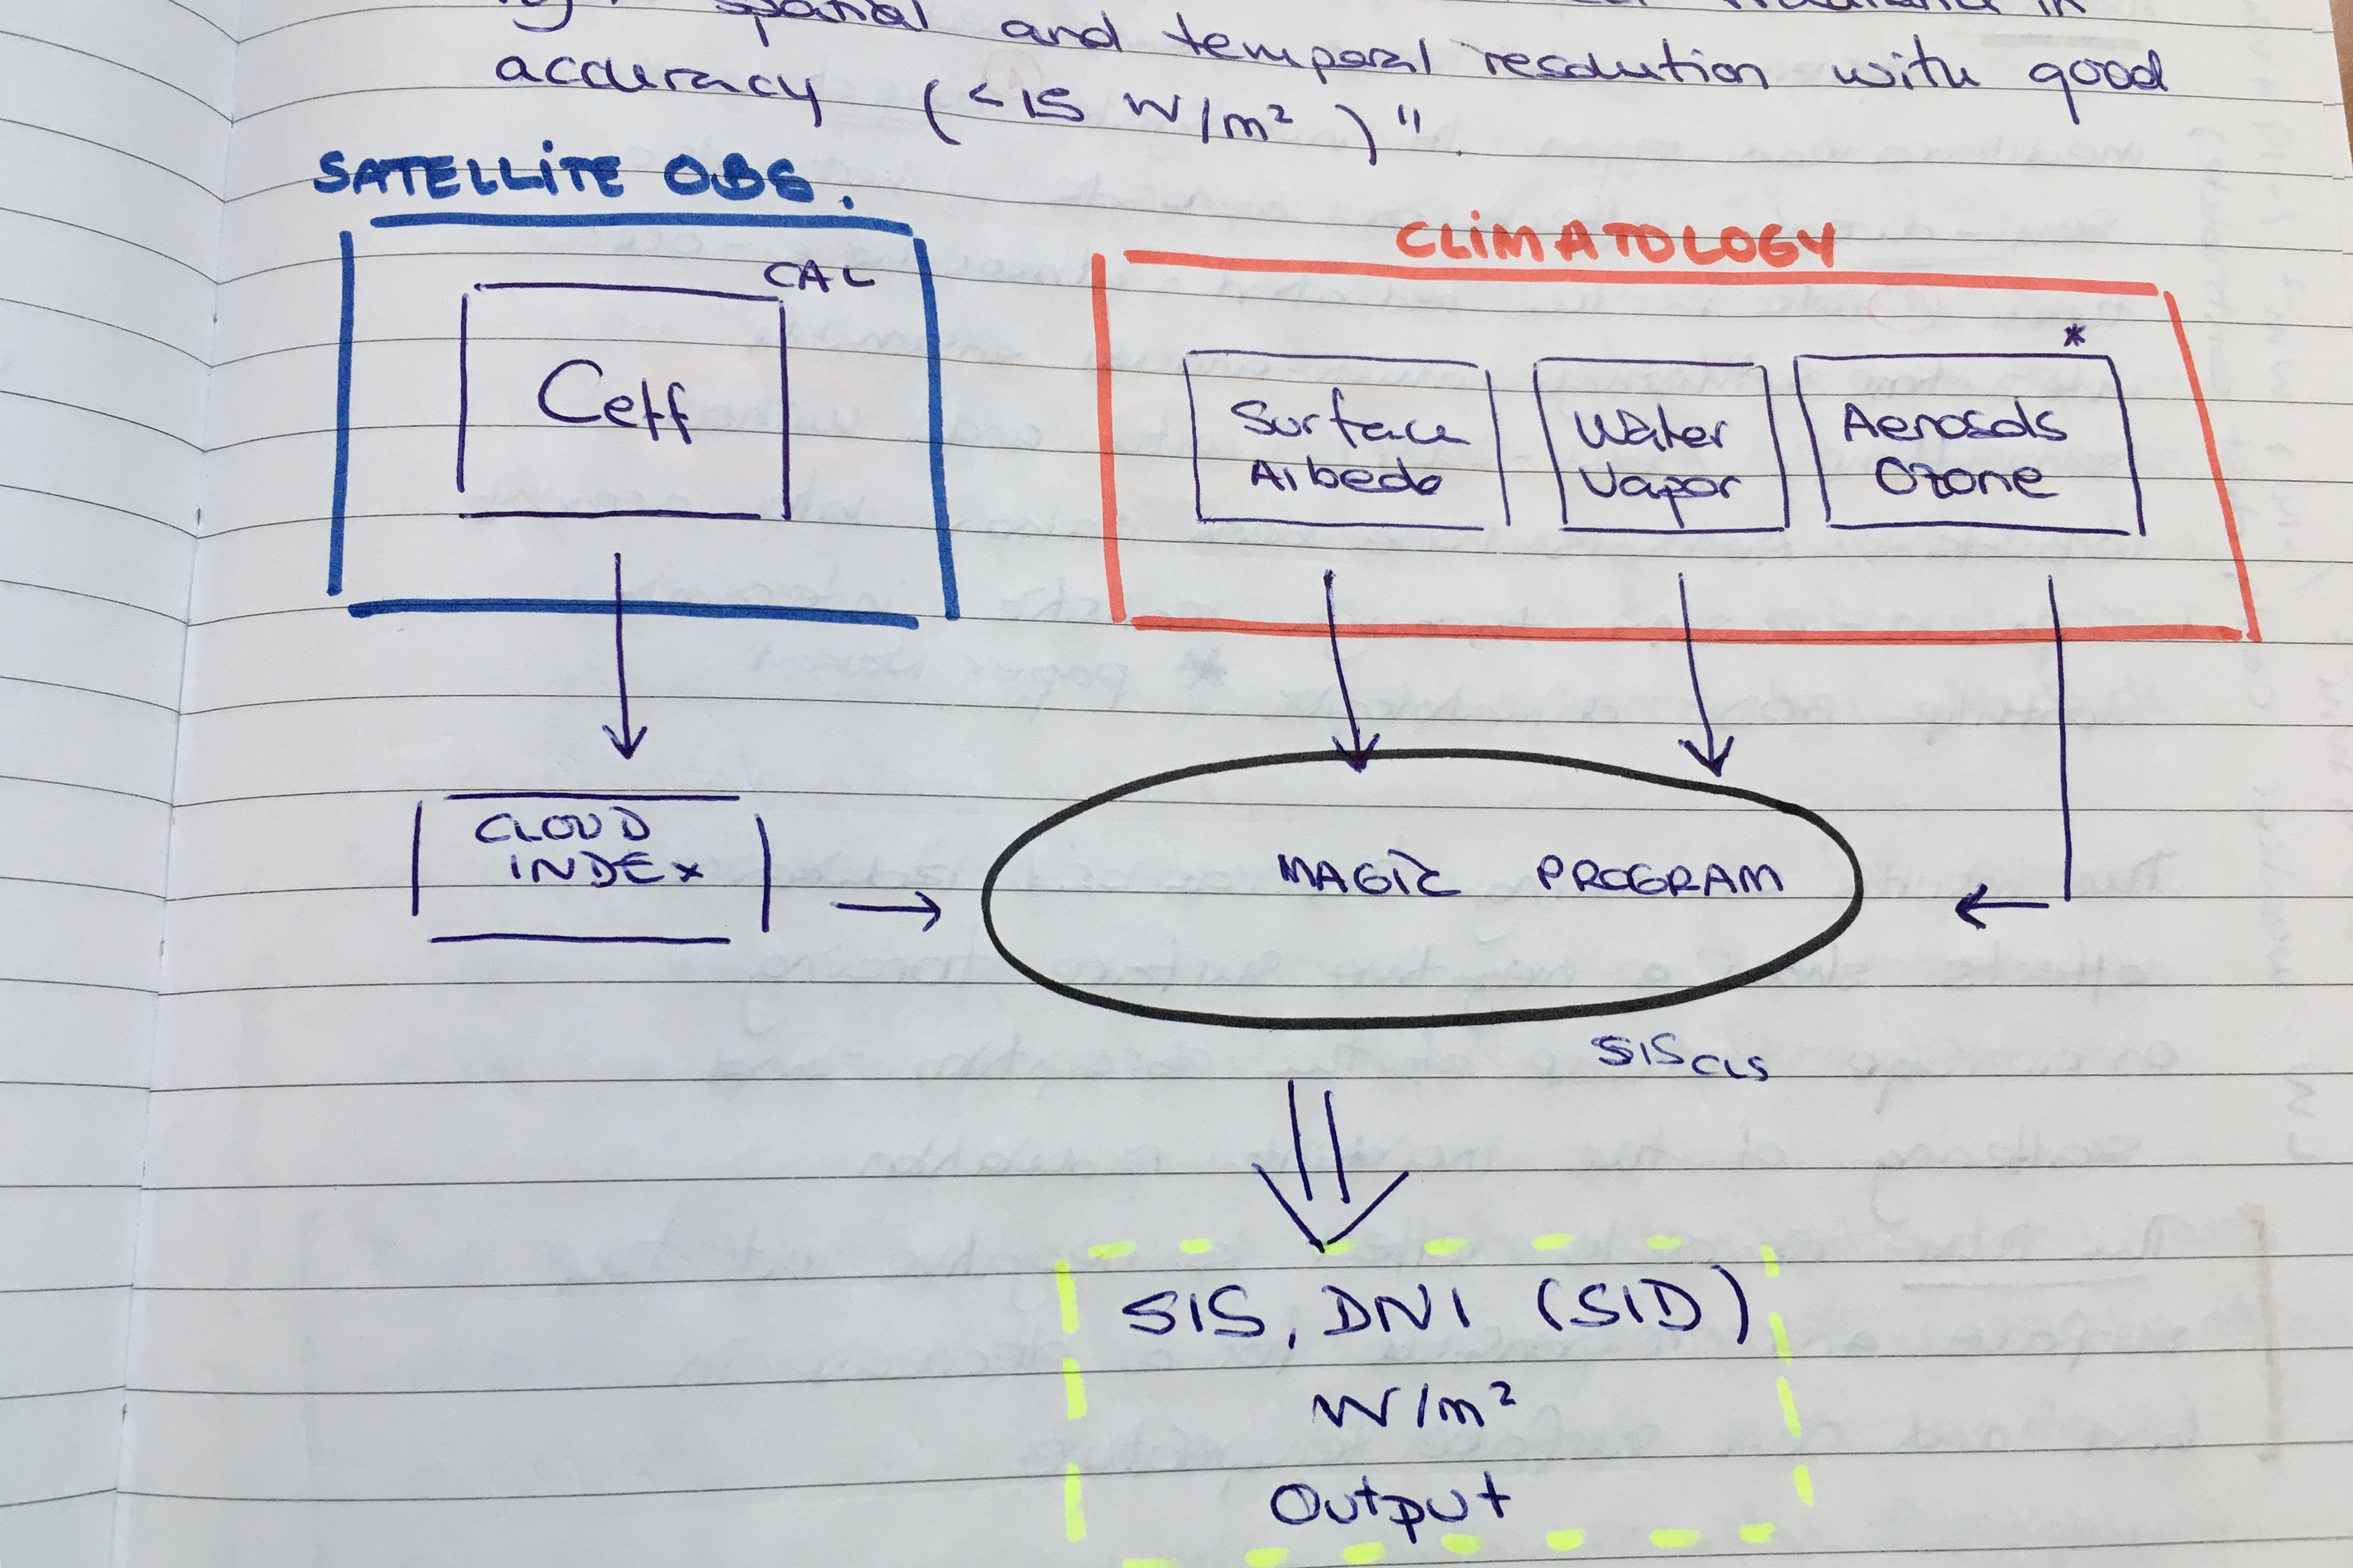
\includegraphics[width=0.6\textwidth]{figs/esquema.pdf}
\caption{Scheme: }
\label{fig:feedback}
\end{figure}

Debido a las características intrínsecas de los recursos renovables relacionadas con su alta variablidad espacio-temporal, el sector energético demanda análisis y conocimiento profundo acerca de éstas caracteríticas en distintas escalas temporales. Esto, ayudaría a una mayor integración de las mismas así como a la mejora en la planifición, poniendo cada vez más relevancia en las escalas climáticas.

En la figura... están representados diversos eventos meteorológicos y climatológicos que afectan a la generación energética. El eje 'x' representa las distintas escalas temporales en las que ocurren estos eventos. Es interesante destacar, aunque no es el tema principal de esta investigación, la relevancia de la escala estacional y sub-estacional para la operación de las plantas energéticas de tipo renovable. La mejora en la predicción climática en estas escalas repercutirá de forma directa en la planificación de la operación y mantenimiento, así como ayuda en la gestión por parte del operador de red y mercado. Por ejemplo, conocer con antelación si un otoño va a ser especialmente lluvioso, sirve para predecir la cantidad de electricidad que se puede producir con las centrales hidroeléctricas, haciendo el sistema mucho más eficiente y fiable. 

Uno de los problemas asociados al posible cambio en el medio-largo plazo de los recursos renovables, como puede ser el eólico, es la posible pérdida de rentabilidad de algunos proyectos que actualmente se encuentran en fase final de su vida. La repotenciación de estos proyectos con tecnologías más actualizadas, como puede ser la sustitución por turbinas eólicas de mayor potencia, junto con la prolongación de las concesiones de explotación del proyecto [ref] son una de las opciones que se dan en aquellas plantas de generación que se instalaron hace casi dos décadas. Los cambios en el recurso pueden cambiar las condiciones del proyecto no sólo por la modernización de la maquinaria y tecnología empleada, sino por el recurso disponible en la misma zona.

La bancabilidad[ref] de un proyecto renovable depende de dos factores: en primer lugar su recurso y en segundo lugar, sus beneficios. Los beneficios obtenidos por el proyecto renovable dependerán del periodo de operación y de la cantidad de energía suministrada en este tiempo. Por ello, una evaluación adecuada, no sólo del recurso disponible a lo largo de todo el proyecto, sino de su variabilidad y de las posibles tendencias, es necesario a lo largo del ciclo de vida de la planta, que puede alargarse hasta 30 años[ref].

% !! escalas climáticas: ¿es importante la repotenciacion? tener en cuenta esto? mismo recurso en el futuro?
% !! infraestructuras y extremos climáticos.
\subsection{Climate services}

Con la creciente demanda de información por parte del sector energético de predicciones y proyecciones climáticas, aparece de manera natural la creación de los servicios climáticos para sistematizar, de alguna manera la información necesaria para los distintos stakeholders. 

Como puede observarse en la figure \ref{fig:feedback}, los procesos de interacción entre la sociedad y las variables involucradas en la generación de energía son de doble sentido. Por un lado el abastecimiento dependerá de la disponibilidad de los recursos y por otro, la demanda está directamente influenciada por estos factores climáticos. Teniendo en cuenta esto, el desarrollo de los servicios climáticos debe basar la mejora de sus modelos y por lo tanto, de los productos ofrecidos en estas dos premisas.

La información climática en el sector energético es especialmente relevante para las descisiones estratégicas y la evaluación de riego, las operaciones de trading o la planficación de la operación y el mantenimiento en las plantas de generación (especialmente) renovables.

Es relevante, aunque no es el tema de esta tesis, decir que también otros tipos de generación no renovable pueden beneficiarse de esta información y estar afectados de manera importante por algunos eventos climáticos. Por ejemplo, el aumento de temperatura del aire puede provocar una subida en la temperatura de los ríos, que ocasionalmente repercute en la operación de las plantas nucleares. En estos casos, estas plantas se ven afectadas porque no pueden continuar on las operaciones de refrigeración de los reactores (ref). 

%\section{Resource assessment}
\section{Climate change and the Mediterranean area}

% \begin{itemize}
% \item Cambio climático de origen antropogénico a escala global. Aumento de la temperatura global.
% \item Los impactos del cambio climático ocurren en escalas locales o afectan de manera local a distintas comunidades y poblaciones de una forma desigual, relacionada también con su capacidad de adaptación y resiliencia.
% \item Por las razones mencionadas arriba, la respuesta a los diferentes impactos de cambio climático deben adoptarse de manera local, a pesar de que el consenso sobre la urgencia de actuación sea global y se adopten compromisos globales comunes.
% \item La mitigación de los grandes impactos ocurre en escala regional/local.
% \end{itemize}

El sistema climático ha variado continuamente y de manera significativa a lo largo de la historia de la Tierra. Las variaciones del clima puede explicarse debido a factores o forzamientos externos y la respuesta del sistema climático a los mismos o, por otro lado, puede ser la causa de inestabilidades internas y relaciones no lineales entre los distintos componentes del sistema.

Los distintos forzamientos de origen externo pueden ser factores astronómicos, como los cambios en la intensidad de la radiación solar o en los parámetros orbitales o por otro lado, factores terrestres como la composición de la atmósfera debido a la actividad humana, por ejemplo, o cambios en la superficie terrestre debido al uso de la misma. 

Algunas variaciones del sistema climático ocurren de manera independiente de los forzamientos externos. Estas variaciones tienen su origen en las distintas interacciones no lineales entre los componentes del sistema climático y dan como resultado la variabilidad natural del sistema climático. 

Desde la revolución industrial la Tierra ha experimentado un aumento de la temperatura global que no es posible explicar mediante los forzamientos externos 'naturales'  del clima como cambios en la actividad solar o en las emisiones volcánicas (Bindoff et al, 2013), ni forma parte de la variabilidad natural del sistema. El IPCC en su último informe, asegura que la actividad humana y en concreto las emisiones de efecto invernadero generadas desde la Revolución Industrial (1850) son responsables del cambio climático que ha generado el ascenso de temperatura global y que ha hecho que probablemente los 30 años entre 1983-2012 hayan sido los más cálidos en los últimos 1400 años en el hemisferio norte (IPCC). A pesar de la marcada variabilidad interanual (Stocker et al. 2013), el aumento de temperatura con caracter global en las últimas décadas es evidente. [ref de observaciones globales]

Las consecuencias del aumento de temperatura desde un punto de vista físico dependen de la sensibilidad del sistema a los cambios en la concentración de gases de efecto invernadero. Son numerosos los estudios [ref] que se han realizado para intentar cuantificar el impacto que este aumento de temperatura puede tener en los distintos subsistemas a través de los diferentes mecanísmos de retroalimentación que pueden generarse.

A pesar de la característica global del cambio climático, sus consecuencias e impactos son percividos a escala local y regional. Estos impactos afectan a comunidades y poblaciones de manera desigual dependiendo de su capacidad de adaptación y resilencia. Por ello, la respuesta desde un punto de vista socio-económico para mitigar estos efectos, tiene que venir dada en esta escala, aunque exista consenso sobre la urgencia de actuación y se adopten compromisos comunes.

Uno de los primeros trabajos que intentaba cuantificar el impacto del cambio climático a escala local fue el de Giorgi et. al 2006. En este trabajo, se utilizaba por primera vez un índice (RCCI) para medir de forma cuantitativa y compara geográficamente las zonas más afectadas por el CC. En este aspecto, el trabajo estaba enfocado desde un punto de vista climático, es decir, el índice mide la sensibilidad del clima en esa zona. En este sentido, el Mediterráneo aparecía como una de las zonas más afectadas y desde entonces ha sido denominado como un hot-spot de CC.

Los ensembles de modelos climáticos proyectan escenarios en los que las principales consecuencias del calentamiento global en el área Mediterránea son un descenso generalizado de las precipitaciones, debido a un aumento de la circulación anticiclónica asociada a un desplazamiento hacia el norte de ``Atlantic storm track''. Las temperaturas proyectadas son inusualmente altas con un ascenso especialmente alto en los meses de verano.


\section{Objectives and sceintific questions}%General scientific question: spatiotemporal behaviour of solar resource and photovoltaic production}

Tras esta introducción se puede definir el principal objetivo de esta tesis que en esencia relaciona cuestiones climáticas con la producción de electricidad con energía solar fotovoltaica. En un contexto de cambio y transición energética, el uso de la tecnología fotovoltaia no ha parado de crecer y los distintos escenarios indican que continuará creciento en un futuro. La varibilidad de los recursos energéticos renovables es una de las principales dificultades en su integración masiva en los sistemas actuales de generación eléctrica, y el impacto de esta varibilidad en escalas climáticas no ha sido estudiado en detalle.

El objetivo será determinar las características espacio-temporales del recurso solar en el área Mediterránea y del potencial o productividad fotovoltaico en escalas climáticas además de determinar el papel de los aerosoles en estas características. Se distinguen 3 capítulos que tratan desde distintas perspectivas este tema.

En el primer capítulo de resultados se analizará una estrategia para regionalizar una unidad geográfica con coherencia desde el punto de vista eléctrico en fucnión de sus características climáticas. En concreto se estudia la Península Ibérica por ser un sistema ``casi aislado'' de manera natural por las dificultades de interconexión con el resto del continente Europeo. 

Por otro lado, en el capítulo 6 se estudia el papel de los aerosoles en la variabilidad del recurso y con ello en la producción. La importancia de los aerosoles en escalas climáticas y su impacto geográfico en este capítulo.

Por último, la importancia de la proyección de los recursos renovables en las condiciones de cambio climático queda reflejada en el capítulo 7 dónde se estudia la posible evolución del recurso solar y el potencial fotovoltaico con respecto a las distintas configuraciones de aerosoles climáticos en los diferentes modelos regionales analizados.

\section{Organization of the manuscript}%\section{General scientific question: spatiotemporal variability of solar resource and photovoltaic production}

The manuscritp is organizded as follows:

The first part contains two chapters: the first one is the Introduction, that aims to overlook the context in which the thesis has been elaborated. In the second chapter it is analysed the main contributions related to the this topic over the literature. It will include the main results about intermittency of PV and how the short-term problems has been managed to go through the long-term problems. After that, the climate change perspective over the area and the main results related to solar resources are presented.

The second part includes two chapters including the Data description and the Methodology used along the studies. In this case it is important to remark that each result's chapter contains the Data and Methodology used for that specific chapter. The contents of this part are related to general description of climate data and models.

Results are presented in the third part.

Finally the fourth part contains a chapter with the main conclusions of the thesis and another chapter that summarizes the main questions emerged from the wotk, which will lead future research.

% \section{State of the art}
% \subsection{From short to long term varibility issues}
% \subsection{Solar radiation data measurements}
% \subsection{Satellite data}
% \subsection{Modelization of solar radiation}
% \section{Identification of knowdlege gaps and approach to the problem}
%\subsection{Spatiotemporal long-term variability in an almost isolated area}
%\subsection{Role of aerosols in the spatiotemporal varibility of the photovoltaic energy production}
%\subsection{Future availability of photovoltaic potential}


\chapter{State of knowdlege\label{cha:state}}
\section{Intermittency of PV}
\section{Variability sources in PV}
\section{From short to long term issues}
\section{Climate Change perspectives for solar resource and photovoltaic potential}

%\end{document}
%\ClearShipoutPicture

\part{Data \& Methods\label{cha:data}}

%%%%%%%%%%%%%%%%%%%%%%%%%%%%%%%%%%%%%%%%%%%%%%%%%%%%%
\chapter{Data\label{cha:data}}
\section{Solar radiation measurements}
\section{Satellite data}
\section{Modelling solar radiation}
\section{photovoltaic prodution data}

%%%%%%%%%%%%%%%%%%%%%%%%%%%%%%%%%%%%%%%%%%%%%%%%%%%%%

\chapter{Methods\label{cha:methods}}

\begin{abstract}

  Para cumplir los objetivos planteados en la presente tesis es necesario el empleo de diferentes metodologías en cada uno de los capítulos de resultados, todas ellas explicadas en detalle en las correspondientes secciones. De manera general el cumplimiento de estos objetivos pasa por el análisis estadístico de las diferentes variables relacionadas con el recurso solar así como de la producción fotovoltaica, siendo esta última una estimación obtenida a partir del modelado de la misma. El análisis se realiza en escalas espacio temporales diferentes, lo que desemboca en la necesidad de utilizar adaptaciones de una misma metolodogía para cada caso.\\

  En el primer capítulo, se analizará de manera espacial la variabilidad interanual y la complementariedad del recurso solar en la Península Ibérica, para lo que se aplicarán técnicas de \textbf{clustering}. La evaluación de la productividad fotovoltaica lleva asociada la necesidad de la \textbf{modelización de un sistema fotovoltaico}.\\

  En el segundo capítulo se estudia el impacto de los aerosoles en la producitvidad fotovoltaica, esta vez en el área Euro-Mediterránea. En este caso, las \textbf{simulaciones climáticas} serán utilizadas como input del modelo fotovoltaico, creando una cadena de modelado que permita realizar un ejercicio comparativo de sensibilidad para cuantificar el papel de los aerosoles.\\
  
  Por último, se realiza el análisis del potencial fotovoltaico futuro, evaluando las tendencias y anomalías con respecto a un periodo de referencia. En este caso, se hace un \textbf{estudio multimodelo} a través de distintas simulaciones de diferentes RCMs que permita evaluar el recurso solar y se utilizan las mismas para el cálculo de la producción fotovoltaica. En este último punto vuelve a considerarse la representación del campo de AOD dentro de las simulaciones climáticas como variable determinante en las proyecciones de SSR y productividad PV.\\
  
\end{abstract} 
\section{Clustering algorithm applied to climate data}
% The culstering algorithms are design for grouping together variables and recognise patterns between them that are difficult to see at first sigth. This algorithm were first applied in ... and they have grown quickly adapting to a highly data-driven world.

% Pattern recognition: extraer objetos y agruparlos en clases. Dependiendo de las distintas disciplinas, estos objetos pueden ser muy diferentes. Se utiliza el pattern recognition en el reconocimeiento de imágenes, de palábras, ayuda en el diagnóstico, o para el análisis de bases de datos en data mining. En este último, las aplicaciones van desde la biología a las finanzas o ciencias sociales y en un data-driven world, cada vez adquiere una importancia mayor, transformando los datos en conocimiento.

% En primer lugar, se definen las características que se van a emplear como medida de similitud/similaridad utilizada para la clasificación. Una vez que estas características están definidas, los algoritmos de clustering se encargan de agrupar  estas características.

%En un mundo cada vez más movido por los datos, el reconocimiento de patrones se ha utilizado en  muchas disciplinas, desde la biología a las finanzas o las ciencias socialses, para extraer información relevante de los diferentes conjuntos de datos. Éstas técnicas, ayudan a conocer relaciones difíciles de extraer a simple vista, bien por el volumen de los datos, o por la complejidad de las mismas y la cantidad de variables involucradas. 

In a data-driven world, \textbf{pattern recognition} is being applied to many disciplines from biology to finanze through social science, in order to obtain relevant information from different datasets. These techniques help to understand relationships that are difficult to extract at a first sight, either due to the volume of the data, or the complexity of those relationships and the amount of different variables involved. Behind all the pattern recognition methods rely the simple fact of classifying objects into similar classes.\\

Depending on the a priori information about the data, it is possible to applied a \textbf{supervised} data classification/pattern recognition or \textbf{unsupervised} pattern recognition.\\

In the first stage of a supervised pattern recognition analysis there is the ability to set the measurements that will define similarity between objects, meaning the definition of the features from the dataset. The classification of different objects in the pattern recognition analysis is implemented through these features and its selection. After that, a criteria to optimally divide the features into classes is decided and applied to them. This stage is called the clasifier stage and its complexity increase with the dimensionality of the data.\\

However, if the similarity measurements can not be define first, due to unknown previous labeled data, another approach will be implemented. In that case, the task will consist in identify the similarities afterwards, from a dataset of features, applying clustering algorithms for that purpose.

\subsection{Clustering algorithms}

It is not under the scope of this work to analayse in detail all the clustering methods available, due to the vast number of them and its increasing complexity. However, it is worth it to give an overview of its classification and application in order to better understand the choice made in the study of our problem.\\

There are different types of clustering algorithms based on its application and the criteria applied to construct the clusters. The two main categories are divided in \textbf{hierarchical} and \textbf{non-hierarchical algorithms}, but there are other taxonomies based on the algorithm construction that can be used to classified different methods [ref].\\

The \textbf{hierarchical clustering algorithms} create a number of nested clusters and they can be also divided themselves in agglomerative or divisive. The first one, obtain a smaller number of cluster in each step, whereas the divisive algorithms, works on the other direction.\\

Most of these hierarchical algorithms are variants of the single-link or complete-link algorithms. They have a different way to measure similarity. In the first case, the distance between two clusters is the minimum of all the pairwise distances measured between the objects of the two clusters, in contrast, for the complete-link algorithm the distance is considered the maximum of all the pairwise distances.\\

On the orther hand, the non-hierarchical or \textbf{partitional clustering algoritm}, create a number of non-overlapping clusters. These methods could be useful when the amount of data involved is large and the construction of a dendogram, produced by the hierarchical algorithm could be computatinal expensive.\\

The partitional methods create the group of clusters using an \textbf{optimization function} which defines the similarity. The main inconvenient of these algorithms is the in advance definition of the number of clusters. Usually, the algorithm is implemented several times for a wide number of partitions and the optimum number of clusters is defined afterwards using validity indexes criteria.\\

{\color{red}{Añadir algo más sobre algoritmos partitional}}


\subsection{Clustering climate data}

As previously commented, the use of pattern recognition and in particular, the clustering analysis, has been widely used across many different disciplines. The use of these techniques to group together atmospheric variables that could help in environmental classifications is a more recent research field.[ref]\\

Historically, the climatic divisions were based mostly on the differences in vegetation types around the globe. The Koppen-Terawata classification [ref] is the most widely known climate classification and bases its divisions in obtaining the vegetation thresholds from precipitation and temperature data. Some authors had already pointed the limitations of this classification method mostly due to two aspects: the first one is that vegetation thresholds are not well defined and that could be an issue when higher spatial resoultion scales want to be defined. On the other hand, is the fact that not only precipitation and temperature are influencing the vegetation species but also other atmospheric variables like solar irradiation, as well as other environmental factors that could be related to antropoghenic emissions or waste.\\

{\color{red}{Buscar más biblio de esto}}

As these classical division are not adapted to the necessities of different fields and could be even biased, another way to geo-spatial classification is needed. In this sense it has become frequent to sucessfully use data-driven classification of different variables if it is necessary to give an spatially resolved answer. [ref]

\subsection{Applied clustering method}

In this work a clustering method is applied to classify solar irradiation due to the fact that classical climate division are only based on temperature an precipitation. The spatial pattern tha could be extract from the Koppen-Terawatta classification, can not be used for our pourpose.\\

A partitional commonly used clustering method has been selected to classify solar irradiation of the area. The \textbf{'k-means'} algorithm is easy to implement, due to the fact tha has been largely used over the literature. Moreover, the combination of a \textbf{principal component analysis} of the dataset previous to the k-means algorithm application has been proved to be an useful tool to reduce the data-dimensionality and apply the algorithm in a more efficient mamner.

\subsubsection{K-Means algorithm}

The k-means algorithm is a partitional clustering method that provide a set of partitions from the application of an optimization function, usually the euclidean distance. The algorithm initiates from a pre-defined number of clusters, 'k', and randomly selects a group of centroids equal to the number of clusters. The optimization function is applied to assign each object to one of the clusters, depending on the similarity (distance) to each of the centroids. This proccess is applied until the algorithm converges.\\

One of the limitations of these method is its dependency on the first selection of the centroids, that could lead to a local optimum instead to a global optimum. To solve these difficulty, the algorithm can be run many times to test the sensitivity of the algorithm to a different initial conditions. Another option is to use an initialization technique to select the centroids.\\

{\color{red}continuar}

\subsubsection{Principal Component Analysis}

The Principal Component Analysis, PCA [ref], consists in a decomposition of the dataset into a number of vectors whose linear combination represents the original data. The transformation of the original data into a lower dimensional space is a reduction of the dimensionality retaining the maximum of the data variance.\\

The new orthogonal system has in its first coordinate axis, the projected values of the original data that preserve most of the variance in the dataset, and it is called the principal component. The rest of principal components decrease the amount of variance explained consecutively.\\

The PCA has been applied in advance to K-means clustering algorithm among the literature [ref]. It was explained by [ref] that the reduction in dimensionality is directly linked to K-means due to the fact that the clustering membership indicators are actually the eigenvectors given by the PCA. For this reason, it has been applied before the K-means algorithm fastening the algorithm.\\

\subsubsection{Validity Index}

\subsubsection{Initialize K-Means}

\section{Regional Climate Modeling}

El sistema climático y su modelización. Modelos de circulación globales. Orígenes de los modelos de área limitada, LAM. Downscalling dinámico que pasó a ser el desarrollo de los RCM.

\section{Simulating a photovoltaic system}

In order to estimate the amount of energy produced by a photovoltaic system it is necessary first to assess the amount of energy that reach the generator surface (plane of array irradiation, $G(\alpha, \beta)$) and after this estimation, which it is not straightforward unless it is measured, the different components of the generator has to be modeled.\\

For the evaluation of the photovoltaic \textbf{energy yield}, defined as the amount of energy produced by a photovoltaic system divided by its nominal power, along this work we use the process explained below, which can be summarized in two steps:

\begin{enumerate}
\item To calculate the \textbf{effective irradiation}, $G_{eff}(\alpha, \beta)$, which is the effective irradiation after substract optical losses, due to reflection, angle of incidence ot dirtiness. The assessment of this variable has to be done from the global irradiation at the surface, $G(0)$, that can be obtain from measurements, atmospheric models or satellite datasets.
\item The second step consists in simulate the \textbf{electrical performace} of the system and estimate the power from the generator. The whole photovoltaic system includes the generator, the inverter and the transmission elements and wires.
\end{enumerate}

All the processes involved in the stage of simulating a photovoltaic system in this thesis have been made using solaR [ref], an R package that implements all the necessary functions to estimate the energy provided by the sytem.

\subsection{Global effective irradiation}

Assessing the amount of energy reaching cells of the photovoltaic generator requires to compute trackers movements, as well as the relative position between sun and panels throughout the year, a detailed description of these methods can be found in \citep{Perpinan.Marcos.ea2013}.  Once these equations are computed, the procedure is described below:

\begin{itemize}
\item First, global irradiation on the horizontal plane is decomposed in two components, \textbf{direct} and \textbf{diffuse} irradiation, Eq.\ref{GlobalIrradiation}. To estimate these quantities it is necessary to consider equations proposed by \cite{Liu1960} to characterize solar irradiation. Definition of \textit{clearness index}, Eq.\ref{K.indicedeclaridad}, is the ratio between global irradiation and extra-terrestrial irradiation at the horizontal plane. They also proposed to relate that index with the \textit{diffuse fraction}: the ratio of diffuse to global irradiation in Eq.\ref{F.diffusefraction}. This relation varies depending on the time scale. For daily values, we estimate correlation between the clearness index and the diffuse fraction using equations in \cite{Aguiar1992}. After that, the diffuse component is obtained with the definition of the \textit{diffuse fraction}, Eq.\ref{F.diffusefraction}.

\begin{equation}\label{GlobalIrradiation}
G_{d}(0) = B_{d}(0) + D_{d}(0)
\end{equation}

\nomenclature[G]{$G(0)$}{Global irradiance on the horizontal plane.}
\nomenclature[Gd]{$G_{d}(0)$}{Daily global irradiation on the horizontal plane.}
\nomenclature[D]{$D(0)$}{Diffuse irradiance on the horizontal plane.}
\nomenclature[Dd]{$D_{d}(0)$}{Daily diffuse irradiation on the horizontal plane.}
\nomenclature[B]{$B(0)$}{Direct (beam) irradiance on the horizontal plane.}
\nomenclature[Bd]{$B_{d}(0)$}{Daily direct (beam) irradiation on the horizontal plane.}


\begin{equation}\label{F.diffusefraction}
F_{D,d}=\frac{D_{d}(0)}{G_{d}(0)}
\end{equation}

\begin{equation}\label{K.indicedeclaridad}
K_{Td}=\frac{G_d(0)}{B_{0d}(0)}
\end{equation}

\item Secondly, daily irradiance has to be estimated from irradiation values. Considering low variability of solar irradiance, it is assumed that average irradiance in a short interval coincides with irradiation in that interval. Regarding equations proposed by \cite{Aguiar1992}, the ratio of the diffuse irradiance to diffuse irradiation is assumed to be equivalent to the ratio of extraterrestrial irradiance to extraterrestrial irradiation Eq.\ref{ratioB0}, and the ratio of global irradiance to daily global irradiation is followed from the same reference Eq.\ref{ratioG0}. 

\begin{equation}\label{ratioB0}
r_{D}=\frac{D(0)}{D_d(0)}=\frac{B_0(0)}{B_{0d}(0)}
\end{equation}


\begin{equation}\label{ratioG0}
r_G=\frac{G(0)}{G_d(0)}=r_D\cdot(a+b\cdot\cos(\omega))
\end{equation}

\nomenclature[Ktd]{$K_{Td}$}{Clearness index.}
\nomenclature[Fd]{$F_{D,d}$}{Diffuse fraction.}
\nomenclature[B0]{$B_0(0)$}{Direct (beam) extra-terrestrial irradiation.}
\nomenclature[B0d]{$B_{0d}(0)$}{Daily direct (beam) irradiation.}

\item The third step considers only geometrical criteria to compute the direct and diffuse irradiance components at the inclined plane.
  Diffuse irradiance is calculated with the anisotropic model proposed in \cite{hay1985estimating}. 

\item The last step estimates the effective irradiance incident on a generator subtracting dust and angle of incidence losses from the incident irradiance with the model proposed in \cite{Martin2001}.

\end{itemize}

In figure \ref{fig:algorithm_outline} the steps to assess effective irradiation at the plane-of-array is summarized.

\begin{figure}
  \centering
  \includegraphics[width=0.6\textwidth]{figs/algorithm_outline}
  \caption{Algorithm scheme: steps on the calculation of global effective irradiation, incident irradiation at the inclined plane. Orange color means input of the calculation and blue color output or results. If a result in a previous step is used in the next one, arrows linking steps are orange. Right side of the scheme represents the method and equations needed.}
 \label{fig:algorithm_outline}
\end{figure}

\subsection{Photovoltaic energy yield}

Once the effective irradiation that reach solar cells is being assessed, the transformation into power output depends on some factors regarding the photovoltaic system. In order to estimate  potential for photovoltaic production, the term yield is defined as the energy produced by the power installed $[\si{\kilo\watthour\per\kilo\wattpeak}]$. That energy, comes from the integration in each time step of the power output of the photovoltaic system.

Considering that reach photovoltaic generator is composed of modules, the generator nominal power output is calculated by multiplying the power output of a module by the number of modules, assuming the same electric performance of all modules. 

\begin{equation}\label{Pout}
P_{out}=I_{m} \cdot V_{m}
\end{equation}

\nomenclature[P_out]{$P_{out}$}{Power output from the photovoltaic module}
\nomenclature[Im]{$I_m$}{Intensity from the photovoltaic module}
\nomenclature[Vm]{$V_m$}{Voltage of a photovoltaic module}

Ambient temperature influence cells performance. The assumption used to this assessment consider a linear relationship between cell temperature and global effective irradiation, Eq.\ref{Tcelula}. NOCT in equation \ref{Tcelula} is considered constant being the temperature of a cell when it works in determined conditions: irradiance of 800 $[\si{\watt\over\metro^2}]$ and ambient temperature of $20ºC$.

\begin{equation}\label{Tcelula}
T_c=T_a + G_{ef} \cdot \frac{NOCT-20}{800}
\end{equation}

\nomenclature[T_c]{$T_c$}{Cell temperature}
\nomenclature[T_a]{$T_a$}{Ambient temperature}
\nomenclature[G_ef]{$G_{ef}$}{Global effective irradiation}

After considering all these factors, the power output of the whole system is assessed by the consideration of a common inverter for transforming DC current into AC, also arrangement losses of the generator are included. Other systems factors that influence the performance of the photovoltaic system are shadows over the generator due to the positions of the PV modules over the land. This factor is not consider in our calculations assuming that we look for an estimation of the potential yield of an area, not the product of a real PV plant. Detailed description of the software employed to the assessment, solaR, is in \cite{Lamigueiro2012}. The process for the photovoltaic output is summarized in table \ref{tabla1} including all the steps and elements involved as explained in \cite{Perpinan2009}.

\begin{table}
  \begin{tabular}{>{\raggedright}m{6cm}>{\raggedright}m{6cm}}
    \toprule 
    Element & Method\tabularnewline
    \midrule
    PV generator & Identical modules with
    $dV_{oc}/dT_{c}=0,475\frac{\%}{\celsius}$ and $NOCT=47\celsius$. 
    The MPP point calculated as in \cite{garcia2005caracterizacion}). \tabularnewline
    \midrule
    Inverter & Efficiency equation proposed in
    \cite{jantsch1992results}:  
    \begin{equation}
      \eta_{inv}=\frac{p_{o}}{p_{o}+k_{0}^{o}+k_{1}^{o}p_{o}+k_{2}^{o}p_{o}^{2}}
    \end{equation}
    where $p_{o}=P_{ac}/P_{inv}$ is the normalized output power of the inverter. The characteristic coefficients of the
    inverters are: $k_{0}^{o}=0.01$, $k_{1}^{o}=0.025$, $k_{2}^{o}=0.05$.\tabularnewline
    \midrule
    Other losses & \begin{itemize}
    \item Average tolerance of the set of modules, $3\%$.
    \item Module parameter dispersion losses, $2\%$.
    \item Joule losses due to the wiring, $1.5\%$.
    \item Average error of the MPP algorithm of the inverter, $1\%$.
    \item Losses due to the MV transformer, $1\%$.
    \item Losses due to stops of the system, $0.5\%$.
    \end{itemize}
    \tabularnewline
    \bottomrule
  \end{tabular}
  \caption{Calculation procedure for the estimation of energy produced by a PV
    system from daily global horizontal irradiation data. Left column represents the element of the PV system and the right column the equations and methods used in each case for the efficiency of the elements.}
  \label{tabla1}
\end{table}

\nomenclature[Pinv]{$P_{inv}$}{Nominal
  power of the inverter}
\nomenclature[po]{$p_{o}$}{Normalized output power of a inverter}
\nomenclature[kinv]{$k_{i}^{o}$}{Coefficients of the
  efficiency curve of a inverter}


\section{Future projections and scenarios}



\part{Results}

%% This part has the 3 chapters related to the main results. Each chapter has the results from one of the papers prepared.
\chapter{Long-term characteristics of solar resource over the Iberian Peninsula}

\begin{abstract}
%     {\color{red}QUÉ HAY AQUÍ:
%     \begin{itemize}
%     \item El estudio se basa en productividad en lugar de en radiación.
%     \item Overview de la radiación en largo plazo. Relacionarlo con la nubosidad, con los aerosoles. 
%     \item Metodología extrapolable para otros estudios en distintas escalas tanto temporales como espaciales. Y también para otras energías.
%     \item cuestiones difíciles: no se ha calculado cv para los periodos climatologicamente estables. ¿Hay variaciones decadales? Wild indica que el recurso debe estudiarse solo con los 10 años anteriores! ver la complementariedad con esto.
%     \end{itemize}}

  % ** En este capítulo se ha elaborado una meodología que puede aplicarse al análisis de cuestiones energéticas relacionadas con el largo plazo y escalas temporales climatológicas. Por ejemplo: el estudio de la variabilidad interanual o decadal de los recursos de energías renovables, así como de la producción eléctrica con éstas tecnologías. El método utiliza técnicas de clustering, lo que permite la evaluación espacial de estas cuestiones. Además, posibilita indagar en estudios de complementariedad de distintas fuentes, gracias a la simplificación de la estructura espacial aplicando las técnicas de agrupamiento.

  % ** Este capítulo contiene una nueva perspectiva para el análisis cuestiones climatológicas relacionadas con la producción renovable: esto implica una manera alternativa de analizar: tendencias de la radiación, tendencias de la producción, relación con patrones atmosféricos, complementariedad etc.

  % ** Se puede analizar la influencia de distintos patrones sinópticos sobre la producción eléctrica con energías renovablesen el área de estudio.

  % ** Se puede analizar la influencia de los modos de circulación en grandes escalas

  % ** Con este trabajo, se puede estudiar si las distintas conclusiones que se han encontrado en relación con el recurso en el área sur de Europa, o PI se observan de manera diferenciada en los clusters de la Península, de tal manera, que esta clasificación sirva para tomar decisiones de gestión de produción o de implantación de plantas futuras. Además, el cálculo de la produción eléctrica potencial, permite ir más allá en la evaluación de ciertas métricas como la variabilidad, ya que muchos de los efectos observados en el recurso, se ven amplificados cuando se hace el cálculo de producción.

  % *** ¿Puede el análisis de clustering encontrar zonas diferenciadas de variabilidad interanual?
  % *** ¿Puede el análisis de clustering encontrar zonas de complementariedad del recurso solar?
  % *** ¿Se observan en las distintas zonas la influencia de patrones sinópticos para las distintas estaciones?
  % *** ¿Se observan en las distintas zonas la influencia de los modos de circulación atmosférica como la NAO?
  % *** ¿Es extrapolable el método a otras zonas?
  
The spatio-temporal characteristics of different renewable resources like solar radiation, wind and precipitation are very different among them and a detailed understanding of each is important for an adequate planning and management of the electricity system. In this chapter, we elaborate a comprehensive methodology to analyse variability and complementarity of PV production that can be applied for long-term energy questions and for climate scales, but it is not limited to those time-scales or to solar resource thanks to the flexibility of the method.\\

The work is focused on solar irradiation as source of energy for photovoltaic (PV) generation over the Iberian Peninsula, IP, and on photovoltaic productivity, which is defined as the amount of energy generated normalized by the installed capacity at each location.  The IP is an interesting site due to the fact that it is a large area with limitations in the interconnectivity with the rest of the European continent. It is also a complex climatic area [] due to its geographical location and its orograhy, which makes it interesting for testing the methodology.\\%  \textbf{A comprehensive methodology to analyze variability and complementarity of solar resource and PV production among sub-regions of this area is developed.}

% The photovoltaic energy yield is defined as kWh per kW installed, which facilitates the comparison among sub-regions and allows a comparison with other renewable energies like solar thermoelectric or wind energy.

% \textbf{The multi-step approach facilitates the spatial evaluation and comparison among areas and it could be applied to different time resolutions, from a short term analysis to climatological perspective as well as a climate change projections analysis.}
The main steps of the method are the application of an objective clustering algorithm for performing a regionalization of the whole domain, the analysis of the temporal variability of solar radiation and photovoltaic energy yield, and the intercomparison of the obtained clusters for examining their complementarity.\\

\textbf{The approach applied in this chapter means a different perpective to analyse the long-term issues in solar resource as the interannual variability, the influence of the large-scale circulation modes, trends or the synoptic patterns related to its variability. The use of the multi-step scheme allows to simplify the spatial analysis and answer the questions from a more applied point of view.}\\

% Dar los principales resultados en el abstract
  
Data from a satellite dataset of 30 years, which is usually considered as the time for defining a climatology, is used inthis chapter and a long-term overview of solar radiation variability is analyzed over the Iberian Peninsula (IP). The spatial distribution and variability of photovoltaic (PV) power yield is calculated for different tracking systems. The variability is analyzed on an interannual time scale, which is relevant for energy supply security and year-to-year price stability. It shows robustness and stability of solar radiation and PV production on average for the whole domain, but with significant differences among clusters that could allow spatial compensation of PV production. The relationship between the variability of solar irradiation and of PV yield is not uniform among the different clusters. Areas where solar irradiation is higher are more sensitive to tracking type.\\

The whole process described in this chapter provides the information of how solar resource and the PV energy yield perform in a limited area and provide the tools to analyze the relationships between sub-areas and their variability. In this sense, this method can be applied for isolated or nearly isolated electric systems located in regions with a variety of climates, or for interconnected systems involving several countries.\\ 

%{\color{red}PRINCIPALES RESULTADOS DE LA IP}  

\end{abstract}  

%\clearpage
\section{Introduction}

%In the past few decades, there has been an increase in the renewable energies installed capacity. Renewable technology prices have decreased rapidly attracting investors to the sector, and political agreements such as the requirements of the European Commission for 2020 are also driving this trend. For photovoltaic (PV) energy a large growing trend is expected in the next years \citep{eurostat2014chap124}. 
% {\color{red} \begin{itemize}
% \item eliminar todo lo que hay en la introducción que sea general y pueda ir en la intro del principio
% \item añadir información sobre la evolución de la fotovoltaica en españa
% \item añadir en la intro pq españa es interesante climatológicamente
% \item añadir pq se utiliza satélite  
% \end{itemize}}


The natural variability of renewable energy resources like solar radiation and wind presents some challenges for the management of electricity systems, which were designed for conventional technologies like nuclear or thermal power plants. For that reason a thorough knowledge and understanding of space-time features of solar radiation is needed. In the case of solar PV energy,  its variability \citep{Widen2015} can be studied from the perspective of the resource or from the perspective of the PV power output, that includes some aspects of the PV generators involved in variability, like inverters or tilted and tracking panels which increase the complexity of the assessment. There are many studies focused on the short-term variability \citep{Zamo.Mestre.ea2014} that analyzed PV production ramps due to changes in solar incident irradiation associated with cloud motion \citep{Cros2014, IEA-PVPS-T14-1.32015}. Also, the smoothing effect that a well-spread site planning has on the PV production is being investigated \citep{Marcos2012, Perpinan.Marcos.ea2013}.\\

Not only short-term scales are important to address renewable resources intermittency but also longer time scales are relevant in order to make the system more efficient and reliable \citep{Davy2012}. Policymakers, transmission system operators and investment companies, need an accurate evaluation of resources availability in present and future climate conditions for their mid and long-term planning. The analysis of interannual variability has a particular importance in order to assess stability of the resource and the financial viability of renewable energy plants \citep{pryor2006inter}, as well as the likelihood of strong electricity price oscillations like the ones associated for example with the large interannual variations of hydroelectric production.\\

Regarding that perspective of long-term variability of solar resources, there are studies focused on long series from stations \citep{Sanchez-Lorenzo2009, Sanchez-Lorenzo2013, vazquez2012interannual} or reanalysis data that identify low frequency changes in solar radiation, as the “dimming” and “brightening” periods \citep{Wild2005}, that show relationship between solar irradiation and anthropogenic aerosols \citep{Nabat2014a}. Some studies examine the influence of large-scale circulation atmospheric modes like the NAO (North Atlantic Oscillation) on solar radiation \citep{Pozo-Vazquez2004, Jerez2013}, while others study the spatial variability instead of the temporal variability \citep{Gueymard.Wilcox2011a}.\\ 

Some authors make use of regionalization techniques for atmospheric variables in order to analyze them from a climatological point of view \citep{Argueso2011} or for solar energy purposes, mainly for operation and short-term assessment \citep{Zagouras2013, Zagouras2014, Zagouras.Pedro.2014}.\\

In this chapter a multi-step scheme that systematizes the time-space comparison of solar irradiation or photovoltaic productivity among sub-regions of the target area is described, taking into account a large set of factors involved in PV production that could affect the variability of photovoltaic energy yield. Spatial complementarity between clusters is analyzed through correlation coefficients of solar irradiation and PV energy yield time series, showing possibilities for compensating PV production shortages in certain clusters.\\

The analysis over the Iberian Peninsula show that most of the results obtain in previous studies can be also seen with this approach. In addition, the methodology allow to give a clearer spatial answer to the questions as well as to sistematize the procedure.\\

%As an implementation example, we have performed a long-term analysis of interannual variability of PV energy yield over the Iberian Peninsula, IP, which has a special interest as a nearly-isolated electrical system with a high solar energy potential and a variety of different climates. The use of satellite data in the case of study is explained due to the fact that in some regions there are not enough well-distributed ground stations with long records of solar irradiation. For this kind of study, where spatial features are important, gridded data from satellites are a high quality alternative data source.

This chapter is organized as follows: in first place, a description of the methodolgy is presented. Each stage of the multi-step scheme is summarized in section \ref{Methods} and explained in more detail in the Methodology chapter. After that, the clustering algorithm is applied to the irradiation over the Iberian Peninsula and main results are shown.\\

\subsection{Methods}

The whole comprehensive scheme followed is represented in figure \ref{fig:multi_step}, showing the 4 stages and procedures that will be explained in detail in the following section.\\

From data of solar irradiation on the horizontal plane as the starting point of the method, the most common variable obtained from different data sources, the scheme will provide different outputs that can be used to evaluate resource and PV production:\\

\begin{itemize}
\item Regionalization of the area to facilitate the spatial analysis.
\item Resource and energy yield aggregated by areas.
\item Interannual variability of the resource and the PV production.
\item Evaluation of the complementarity of the resource and PV production among areas.
\end{itemize}  
 
\begin{figure}[h!]
\centering\includegraphics[width=1\textwidth]{figs/capitulo5/multi_step}
\caption{Scheme: Each gray block represents each of the operations needed to get the variability and complementarity results. Orange ellipses are the data employed and blue ellipses are the results of each stage. If the results of one of the blocks are used as input for another stage, connectors are represented in orange color.}
\label{fig:multi_step}
\end{figure}

\subsubsection{Regionalization by clustering}

Regionalization procedures provide the ability of extracting general information of the areas that could be treated as a coherent unit, facilitating the analysis and not considering those characteristics that are not under study. As it was explained in the methodological chapter, classical climatological classifications have some grade of subjectivity due to the fact that they rely on arbitrary assumptions \citep{Kottek2006} and their criteria are based on temperature and precipitation \citep{trewartha1980koppen}. For our purpose, objective and data-derived criteria are more suitable due to the fact that a different variable is analyzed and its classification does not match classical climate divisions. Objective methods based on clustering techniques have been applied successfully over the literature for the analysis of renewable energy resources \citep{Polo2015}, \citep{Zagouras2013}, \citep{Zagouras2014}, \citep{Zagouras.Pedro.2014}, \citep{gomez2015characterization} and atmospheric variables \citep{Argueso2011}, \citep{garcia2012seasonal}. \\

% Clustering methods \citep{Jain1999} can be divided into two categories, partitional and non-partitional. The partitional clustering divides the data into non-overlapping clusters while, the non-partitional or hierarchical clustering, provides a set of nested clusters. In our case, we made use of both algorithms selecting the hierarchical method to initiate a partitional algorithm that is the most suitable for our purpose: to find spatial regions that group together similar time series of the variable analyzed.

A commonly applied regionalization methodology includes the Kmeans algorithm after preprocessing the data through Principal Component Analysis \citep{Ding2004}. This two-step method first reduces redundant information by a Principal Component Analysis that decreases dimensionality of the original dataset. After that, k-means algorithm is applied to the reduced data to find the optimal partition of clusters, which is based on similarity between each element or object inside the cluster and its centroid. This is considered as the most representative element of the cluster, and similarity is measured by an objective function defined in the cluster algorithm.\\

This method presents some problems regarding the random selection of the cluster centroids in the first step. Different initial centroids can lead to different solution or a local optimum could be found. Also, there could be some computational problems if many iterations are needed to get the final partition.\\

The procedure used in \cite{Argueso2011} and in \cite{Zagouras2014} is adapted to get the optimal partition in our scheme from a combined clustering grouping and avoiding the above mentioned problems: the \textbf{k-means partitional algorithm is initialized with a hierarchical clustering solution of a the dimension-reduced data by a Principal Component Analysis.} For the particular case applied in this work, vectors of daily solar irradiation are used for the regionalization. The following steps are needed to get the optimal partition of clusters in the area:\\

\begin{itemize}
\item \textbf{To reduce data dimensionality}. Principal components are eigenvectors of an orthogonal matrix after applied a singular value decomposition (SVD) to the original data, daily solar irradiation vectors, whose initial dimension is reduced to the first eigenvectors that retain $95\%$ of the variance. Considered that, a linear combination of these eigenvectors represents the initial data.
\item \textbf{Hierarchical clustering to initialize k-means}. A hierarchical clustering method classifies data based on a hierarchy. If it is agglomerative, it will start with a cluster for each observation of the data and observations will group together recursively by similarity using the “complete linkage” method. Once the hierarchy is obtained, centroids can be calculated for each emerged partition with a number of clusters between 2 and \textit{n}, where \textit{n} is a high enough selected number of clusters. Centroids will be the initial seed for the Kmeans algorithm, avoiding the computational problems and favoring reproducibility.
\item \textbf{Kmeans algorithm}. The k-means algorithm is a partitional clustering method that minimizes an objective function that defines similarity among the elements of each cluster. In our case we made use of the Euclidean distance, Eq. \ref{eq:euclidean} between the objects or elements in the cluster and its centroid as the objective function. The number of clusters in which the data is divided into has to be known beforehand. In order to overcome the inconvenience, the algorithm is run from 2 to \textit{n} clusters and the optimum number is determined by making use of a clustering validity index after that.
\begin{equation}\label{eq:euclidean}
    J =\sum_{i=1}^{k}\sum_{j=1}^{n}{||x_i-c_j||}^2
\end{equation}


\nomenclature[J]{$J$}{Objective function of the Kmeans clustering method: summation over euclidean distances}
\nomenclature[x_i]{$x_i$}{Each point in the cluster, where the point is a vector with elements comprising the daily irradiation time series values at a pixel obtained from satellite images }
\nomenclature[c_j]{$c_j$}{Centroid of the cluster j}
\nomenclature[PV]{$PV$}{Photovoltaic}
\nomenclature[IP]{$IP$}{Iberian Peninsula}

\item \textbf{Validity index}. In order to determine the optimal partition, validity clustering techniques are applied. There are two types of validation for the clustering methods. First, external clustering validation that make use of external information out of the data; and secondly, there are internal clustering validation methods that rely only on information from the data \citep{5694060}. The latter are used to preserve objectivity as much as possible and are based on two criteria: compactness and separation of the clusters emerged. We use one of the most applied validity index, the Calinski-Harabasz index \citep{CalinskiH}, CH, that evaluates the average between and within cluster sums of squares.
\item \textbf{L-method}. CH index is calculated for every partition from 2 to $n$ clusters. The resulting CH graph in figure \ref{CHindex} for the Iberian Peninsula regionalization is shown for a number of clusters between 2 and 70 as an example. Theoretically, the partition with the maximum CH is the optimum, but the graph shows a decreasing trend which leads to imprecision in finding the optimum. The large number of data and the continuous variable analyzed are responsible for that. For that reason, the L-method is applied \citep{Salvador2004}. This method selects the intersection of two best-fit lines in the graph CH vs. \textit{k}, where \textit{k} is the number of clusters of the partition \citep{Zagouras2013}. All possible pairs of lines that fit linearly to the left and right sequence of data points are created. Each line has at least two points. The total root mean squared error is calculated as in Eq.:\ref{eq:total_RMSE}:

\begin{figure}[h!]
\centering\includegraphics[width=0.5\textwidth]{figs/capitulo5/CHindex}
\caption{Calinski-Harabasz index by 'k' number of clusters}
\label{CHindex}
\end{figure}
 
\begin{equation}\label{eq:total_RMSE}
  RMSE_T = \frac{c-1}{k-1}RMSE_{left}+\frac{k-c}{k-1}RMSE_{right}
\end{equation}


\nomenclature[k]{$k$}{number of clusters.}
\nomenclature[c]{$c$}{number of clusters where the 2 fit-lines split.}
\nomenclature[CH]{$CH$}{Calinski-Harabasz validity index.}
\nomenclature[RMSET]{$RMSE_T$}{Total root mean square error}
\nomenclature[RMSEleft]{$RMSE_{left}$}{Root mean squared error of the left-side linear regression.}
\nomenclature[RMSErigth]{$RMSE_{right}$}{Root mean squared error of the right-side linear regression.}

Where \textit{c} is the number of clusters where the graph is split into the two fit-lines, \textit{k} is the total number of clusters. The ``total root mean square error'' is a weighted error with two terms, one for each side of c in the graph. Each side has a heavier weight depending on the points involved in the fitting. The minimum of $RMSE_{T}$ gives us the optimum number of clusters of the data \citep{Zagouras2013} which are used in the following steps.
 
\end{itemize}
 
\subsubsection{Photovoltaic energy yield}

The simulation of a photovoltaic energy system is described in a previous chapter. Here it is summarized in order to do not miss the coherence of the text.\\

The assessment of the power output of a photovoltaic system is carried out in two main steps:

\begin{enumerate}

\item In first place, global irradiation on the horizontal plane $G(0)$, which is the most common variable obtained from data sources, has to be transformed into the plane-of-array irradiation,  $G(\alpha, \beta)$, where $\alpha$ is the azimuth angle and $\beta$ the inclination angle of the generator plane. Due to optical losses (reflection, angle of incidence, and dust), the irradiation available is reduced for the photovoltaic cells inside the panels and the plane-of-array irradiation is then denoted as effective irradiation on the PV generator $G_{eff}(\alpha, \beta)$.\\
Three different types of tracking types are considered for the photovoltaic generator that influences on the tilt of the panels:
\begin{itemize}
\item \textbf{Fixed} panels with an optimum angle of inclination that depends on the latitude of the place.
\item \textbf{North-South} oriented panels that track the sun daily varying the azimuth angle, we will refer to them as ``one axis''
\item \textbf{Two-axes} tracking system that allows variation of the azimuth and inclination angles, we will refer to them as ``two axes''.
\end{itemize}
  
\item Once the effective irradiation that reach solar cells has been assessed, second step is the transformation into power output that depends on the photovoltaic system. The photovoltaic system is composed of a PV generator, consisting of several PV modules, and an inverter to transform the DC current output from the generator into AC current to be integrated into the network. In order to estimate  potential for photovoltaic production, the term \textit{yield} is defined as the system energy produced divided by the power installed $[\si{\kilo\watthour\per\kilo\wattpeak}]$.

\end{enumerate}

%The detailed description of the transformation from global irradiation in the horizontal plane to global effective irradiation, as well as the methods to assess power output from the PV generator are in the appendix A.

\subsubsection{Variability and complementarity}

The metric to analyze interannual variability is the coefficient of variation, CV Eq.\ref{eq:CV}, which is defined as:

\begin{equation}\label{eq:CV}
  CV=\frac{\sigma}{\overline{X}}
\end{equation}

In this equation, $\sigma$ is the standard deviation of the variable analyzed and it is divided by the mean of the variable in the period of the study. Sometimes CV is represented in percentage. This measure is dimensionless and can be applied in different time scales, which is helpful for comparisons.\\

To assess complementarity of the solar resource in the area of study, the Pearson's correlation coefficient between the time series of pairs of clusters Eq.\ref{eq:pearson} is calculated:

\begin{equation}\label{eq:pearson}
  \rho_{i,j}=\frac{\sigma_{c_i,c_j}}{\sigma_{c_i}\sigma_{c_j}}
\end{equation}

In this equation, $c_i$ and $c_j$ are the time series corresponding to the clusters $i$ and $j$. The concept of complementarity is associated with negative correlations between sub-regions of a wider area. If there is such a complementarity, a positive change in the variable for one of the clusters will be associated to a negative change for the other one. This is relevant for identifying spatial compensation possibilities and reducing overall variability in a network with high penetration of solar PV energy.\\

Complementarity can occur in different scales, either spatial or temporal and to understand it sometimes is a matter of balance. Spatial resolution for the complementarity assessment must be high enough to make sense of the comparison between zones, due to the fact that it is clear that geographically dispersed areas, far from each other, will have very different evolution of atmospheric variables, but may not be interesting from the electricity generation point of view. On the other hand, if the area of study is too small, atmospheric variables and therefore renewable resources will evolve in a very similar way. For such small areas, local complementarity between different resources can be analyzed, but not spatial complementarity of one resource. The methodology presented here addresses this issue by applying the inter-cluster comparison, that ensures homogenity within each cluster and differences between them.\\

Correlation coefficient for a long time series may hide changes in complementarity for shorter sub-periods with higher frquency correlations. For that reason a moving window is applied to the time series calculating the correlation coefficient and providing an indication of how complementarity between clusters varies during the whole period. Width of the window depends on the length of the time-series analysed.\\

In order to obtain the more important cluster pairs regarding complementarity, the median of the correlation coefficient series is calculated for each pair. After that, the cluster pairs are reordered from lower to higher values of this median correlation.\\
%, and the first 15 pairs (with the lowest median correlation) are selected as the most representative of complementarity, altought this number is rather arbitrary and also depend on the length of the time-series analysed.
 

\subsection{Results}

The optimal partition after having applied the clustering method is represented in figure \ref{clusters}. The CH validation procedure gives an optimum number of 19 clusters for the area, where each of the clusters has an homogeneous time evolution of solar irradiation. Due to the nature of clustering techniques, there is not an unique/best method to select the optimum partition. Another index (Davies-Boudin, \cite{davies1979cluster}) has been applied for comparison, and the obtained optimum number of clusters was of the same order than for CH index.
 
\begin{figure}[h!]
\centering\includegraphics[width=0.6\textwidth]{figs/capitulo5/clusters2}
\caption{Optimal partition of 19 Clusters after applied the algorithm and the validity index}
\label{clusters}
\end{figure}

\subsubsection{Variability and complementarity results}

After regionalization, it is performed an analysis of solar irradiation on the horizontal plane and PV yield by tracking system, including their temporal variability.\\

Regarding interannual variability, we have calculated the CV of two time-aggregated means of solar irradiation and PV yield:

\begin{itemize}
\item On one hand it is applied for the yearly mean of daily irradiation $G_{d,y}(0)$ and yearly PV yield. This metric gives the variation of the of energy from one year to another and if it is low, general stability of the solar resource and PV production is guaranteed. 
\item On the other hand the interannual variability of the monthly time series $G_{d,m}(0)$ and monthly energy yield is also investigated in order to quantify differences in the annual cycle. 
\end{itemize}

The CV is also aggregated by cluster, in order to facilitate the intercomparison among areas.\\

%The general results about yield and variability can be found in the appendix. Here we present particularly relevant results that show the importance of considering different types of tracking methods, which is a fundamental aspect of the proposed scheme.\\

Power from the PV generator depends quasi-linearly with solar irradiation at the plane-of-array ($G_{eff}(\alpha,\beta)$), besides second order effects (spectrum, wind, etc) \citep{Perpinan2007} . Due to that the fixed typology is the one with lower yield because the amount of irradiation reaching cells is lower than the amount of energy reaching panels when trackers have one or two axes movements.

For areas where solar irradiation is higher, yield differences between trackers are higher. This can be seen in figure \ref{yearly_productivity_byCluster} where yearly mean yield for the 30-years period is aggregated by cluster and tracking system, and clusters are sorted vertically from less to more energy yield. A noteworthy result is that yield increase from fixed panels to one-axis panels is non-linear. This increase ranges between $17\%$ for the clusters with less solar irradiation, located at the northern coast (clusters 4, 5), and $30\%$ for the southern clusters with more solar irradiation (clusters 18, 19). In contrast, enegy yield increase from one-axis to two-axes panels is almost constant, around $12\%$ for all clusters. A consequence of the non-linear PV yield increase from fixed to one-axis panels is that the energy yield differences between clusters are much higher for tracking than for fixed systems. While for fixed panels PV energy yield varies between 1000 and 1450 $[\si{\kilo\watthour\over\kilo\wattpeak}]$, for two-axes systems it varies between 1350 and 2100 $[\si{\kilo\watthour\over\kilo\wattpeak}]$. These average values are coherent with results obtained in \cite{Antonanzas-Torres2013} when considering a value of 0.75 for the system performance ratio.
 
\begin{figure}[!tbp] 
\includegraphics[width=0.6\textwidth]{figs/capitulo5/productividadTemp_byCluster.pdf}
\caption{Yearly mean of PV yield by cluster and for each tracking system $[\si{\kilo\watthour\over\kilo\wattpeak}]$. Values are sort from lower to higher yield values.}
\label{yearly_productivity_byCluster}
\end{figure}

Electricity price variations significantly depend on the variations of the monthly renewable electricity production from year to year. This time-scale is also the most influenced by the large scale circulation modes for solar potential in the Iberian Peninsula \citep{Jerez2013a}. The winter half of the year, from October to March, is especially variable.

The interannual variability for monthly yield is higher than for the irradiation at the horizontal plane, as it occurred for yearly values which results are in the appendix. In winter months, these differences in CV are much higher than in summer. This behavior is more pronounced in northern areas.

In order to quantify these differences in variability between solar irradiation and solar power output, the ratio between variability of yield by tracking system and solar irradiation is represented in figure \ref{ratiosCV} for each month and cluster. If CV of energy yield is higher than CV of solar irradiation, values are above one. On the other side values will be below one if CV of solar irradiation is higher than CV of energy yield. 

\begin{figure}
  \includegraphics[width=0.6\textwidth]{figs/capitulo5/dotplot_ratio_zone.pdf}
  \caption{CV ratios between each type of tracking system and solar irradiation at the horizontal plane, grouped together by month in the graph. Ratios are calculated for each cluster, represented in the x axis. ``Fixed'' represents $\frac{CV_{fixed}}{CV_{G0}}$, ``1 axis'' is $\frac{CV_{1axis}}{CV_{G0}}$ and ``2 axis'' is $\frac{CV_{2axes}}{CV_{G0}}$}
  \label{ratiosCV}
\end{figure}

The highest ratios are obtained between $CV_{2axes}$ and $CV_{G0}$. The ratio of $CV_{1axis}$ is clearly lower in winter months, but is very similar in summer to the ratio of $CV_{2axes}$. Yield with an 'horizontal' axis tracker and 'two-axes' trackers increase the variability between $20\%$ in summer and more than $80\%$ in some areas in winter. The fixed typology ratio, $CV_{fixed}/CV_{G0}$ has a much wider range in the whole year. In winter months, it has values between 1.2 and 1.6, depending on the cluster, and is not far from the other two typologies. In contrast, this ratio decreases rapidly in summer months, reaching values below one between May and August. This means that for that period, variability of the 'fixed yield' is smaller than variability of solar irradiation at the horizontal plane.

The results of CV show that variability of PV energy yield at tilt panels is higher than variability of solar resource at horizontal plane in most cases, explained by the nature of solar irradiation at tilt panels and its dependency of solar irradiation at horizontal plane, \cite{Perpinan2009}.

The monthly time series are also selected for the complementarity analysis.

Regarding solar power complementarity, opposite-evolving time-series for different areas would strongly increase the reliability of the whole electric system, as shortfalls of solar irradiation in certain areas could be compensated by above-normal irradiation in others. However, this ideal situation is difficult to find in a rather limited area like the IP, at least for monthly timescales over a long time period of 30 years. In this case, the absence of correlation becomes also important, as it avoids simultaneous shortfalls or simultaneous above-normal values, and therefore softens the overall power production. The correlation matrix for the 30-year period and each month is in the appendix, showing the results for the whole period. In most cases, the correlation coefficient is highly positive, specially between pairs in the northern part of the Iberian Peninsula. For the southern part, the correlation coefficient is also positive but it decreases in July and August. There are some exceptions between the northern clusters 4 and 5 and the southern clusters 14 to 19, these pairs are only slightly correlated, not correlated or even slightly anticorrelated for some months.

Overall, southern and eastern clusters are uncorrelated at least during part of the year with northern and northwestern clusters. In some cases, the absence of correlation is found between nearby clusters: in winter months, the north-eastern cluster 11 (central Ebro valley) is uncorrelated to the closely-lying clusters 4, 5 and 8 (in the northern coast and Pyrenees). This is probably related to persistent atmospheric situations with north to northwesterly winds, that cause cloudiness in the windward clusters and clear skies in the leeward Ebro cluster, due to a foehn effect. This result points out the selective character of the clustering method.

It could be that the obtained clusters present higher complementarity in shorter sub-periods. We have divided the whole 30-year period in sub-periods of consecutive 15 years. The correlation coefficients have been calculated again for the resulting 15-year moving window, for each pair of clusters and for each month. In this way, we obtain how each correlation coefficient evolves during the 30 year period. The analysis has been applied for the four variables in the study: solar irradiation at the horizontal plane and PV energy yield for each tracking system.

The median value of the correlation coefficient series is calculated for each pair. Each serie comprises 12 monthly values for each of the 15-year moving windows. After that, the cluster pairs are reordered from lower to higher values of this median correlation, and the first 15 pairs (with the lowest median correlation) are selected as the most representative of complementarity. These cluster pairs are represented in figure\ref{horizonplot_rad}, showing the time-evolution of its correlation coefficient. These results are for solar irradiation on the horizontal plane. The corresponding figures for PV yield by tracking system are not shown due to the similar results obtained for this analysis.

\begin{figure}[h!]
\includegraphics[scale=0.6]{figs/capitulo5/horizonplot_series_rad2}
\caption{Correlation coefficient of solar irradiation at the horizontal plane: evolution of a 15-year moving window of monthly values, for the 15 cluster pairs showing the smallest median correlation values. Monthly negative correlations (in red) and monthly positive correlations (in blue) are represented in the same axis to facilitate the comparison of the multiple time-series. Also, higher correlation values overlap with lower ones, enabling a compact presentation of all the information in a narrower plot. The cluster pairs are indicated on the left, while the year in the x-axis indicates the end of each 15-year moving window.}
\label{horizonplot_rad}
\end{figure}

The most relevant pairs in terms of complementarity include a northern (1, 2, 4 or 5) and a south-eastern cluster (17 or 18), as can be seen in figure \ref{horizonplot_rad}. The negative correlations for these pairs reach values below -0.6, at least in some 15-year sub-periods. These clusters are negatively correlated in most cases. Clusters 19 and 14 (southern and south-western IP) are also negative correlated with clusters in the north, although with lower values than the south-eastern clusters.

It is important to notice the appearance of cluster pairs 3-4 and 3-5 in this figure. These clusters are closer than the previously commented cases, which highlights the adequacy of the clustering method. All three are Atlantic coast clusters, but while cluster 3 includes part of the western coast, clusters 4 and 5 are northern coast areas. This fact, together with the position of the main mountain ranges, can explain their partially complementary behaviour.

%It is important to notice the appearance of cluster pairs 3-4 and 3-5 in this figure. These clusters are closer than the previously commented cases.  All three are Atlantic coast clusters, but while cluster 3 includes part of the western coast, clusters 4 and 5 are northern coast areas. This fact, together with the position of the main mountain ranges, can explain their partially complementary behavior. On the other hand, the 15-year moving window reveals interesting changes with time for all the cluster pairs, as there are higher and more frequent negative correlations in the middle 15-year sub-periods (those ending around 2005). 

In order to highlight the months with maximum anti-correlation,  figure \ref{horizonplot_months_rad} presents, for the same 15 cluster pairs as above, the minimum values of the monthly correlation coefficient (where the minimum for each month is calculated over all 15-year sub-periods). Differences between months are clearly observed in this graph. Only two months (March and June) show consistently positive values of this parameter, and therefore a low complementarity. In the other months, this parameter has predominantly negative values, revealing a certain degree of complementarity. July, August and September show rather low values and relatively high complementarity, which is important as these are months with a high productivity and also include the summer demand peak. In general,  for the second half of the year, the values of this minimum correlation value are lower than for the first half of the year.

\begin{figure}[h!]
\includegraphics[scale=0.6]{figs/capitulo5/horizonplot_months_rad2}
\caption{Correlation coefficient of solar irradiation at the horizontal plane: minimum values of the monthly correlation coefficient, for the same cluster pairs as figure \ref{horizonplot_rad}. The minimum is calculated over all 15-year sub-periods. The type of representation of correlation values is the same as in figure \ref{horizonplot_rad}. The cluster pairs are indicated on the left, while the numbers in the x-axis indicate the months.}
\label{horizonplot_months_rad}
\end{figure}



\subsection{Conclusion}
\subsection{Summary}

\chapter{Impact of aerosols in photovoltaic energy production over the Euro-Mediterranean area}

\begin{abstract}

The increase in the photovoltaic energy installed capacity over the world leads to the need of a better understanding of solar resource and its variability. The aim of this work is to assess the influence of aerosols on photovoltaic energy production from seasonal to multi-decadal time scales. For this purpose we use various coupled aerosol-climate simulations that take into account the complex spatial and temporal patterns of natural and anthropogenic aerosols over the Euro-Mediterranean domain.

The results show that aerosols strongly influence the spatial pattern, seasonal cycle and long-term trend of PV production. The most affected area is Central Europe where sensitivity of PV production to aerosols is higher. The annual production loss due to aerosols ranges from no impact to $-16\%$ in The Netherlands, with variation depending on the area and on the typology of the tracking system. The summer production loss can even reach $-20\%$ over regions of Africa and Syria-Iraq.  

We conclude that aerosols can not be neglected in the assessment of PV production at large time scales over the Euro-Mediterranean area. Besides, the potential increase in energy due to reduction in the antrophogenic aerosols is shown in the simulation of the brightening period over Europe, with an increase of 2000 ${\kilo\watthour\over\kilo\wattpeak}$ in a PV lifetime for the most affected areas. It illustrates the evolution that PV potential could follow in highly polluted areas through the effective implementation of pollution control measures.  
  
   
\end{abstract}
 
\begin{keyword}
\texttt{Photovoltaic production variability\sep Aerosols\sep Regional Climate Modeling}
\end{keyword}

\end{frontmatter}

\linenumbers

\section{Introduction}


In the last decades there has been an overall increase in the deployment of photovoltaic (PV) power plants over the world, demanding research in the fields that contribute to a better integration of this technology into the electricity system. Due to the variability of solar resource, a comprehensive study of its spatiotemporal behavior is needed.

Aerosols particles influence the climate system directly, affecting the Earth’s radiation budget by scattering or absorption of solar radiation, or indirectly, changing cloud properties. Due to their importance in the amount of solar radiation that reaches the Earth’s surface and their effect in the changing climate, the evaluation of their impact on the solar resource for energy purposes is of special interest.

A general lack of well-spread surface stations, which provide solar radiation measurements, has made the satellite information the main and most reliable source of data up to now, due to its spatial and time resolution \citep{Posselt2012, Ineichen2014}. However, satellite retrievals were not available several decades ago and they do not allow to quantify the effect of specific factors on solar irradiance. Thus for investigating long-term statistics and to disentangle the various factors influencing solar resource, a different approach is needed. Models are the best tool to understand processes that occur in the atmosphere and their link with the resource variability, as individual factors can be included or removed in them, allowing the isolation of their effects.

Due to the increasing concern about the availability of renewable energy resources under climate change scenarios, climate modeling has revealed itself as a valuable tool for evaluating future energy potential \citep{Crook2011, Gaetani2014, Gaetani2015, Jerez2015, Jerez2015climix, Tobin2016}. However, representation of the clouds is still one of the main challenges for these models, and the spatio-temporal variability of aerosols is rarely taken into account in some of regional climate models \citep{Bartok2017}, which could lead to significant errors in PV power forecasting or future energy estimations \citep{Rieger2017}. Such climate simulations have to be combined with an accurate PV model capable of reproducing the system performance. Existing studies analysing the influence of aerosols on solar irradiation lack spatial detail (because of the use of relatively coarse global climate models) and/or do not apply a detailed PV production model \citep{Bergin2017}. 

The Mediterranean region is considered as highly influenced by aerosols coming from different sources \citep{Lelieveld}. These aerosols have a deep impact on the climate of the region \citep{Nabat2014, Nabat2014a}, thus on the shortwave solar radiation reaching the surface \citep{Mallet2016}. Regarding possible changes in antrophogenic aerosols in the future \citep{Gaetani2014, Jimenez-Guerrero2011}, the relevance of the near-term climate change scenarios and the expected PV deployment, the study of the Euro-Mediterranean area is important for solar energy.

In this work we use a regional climate model \citep{Nabat2014} with a realistic aerosol representation combined with an accurate PV model \citep{Lamigueiro2012}. The influence of these aerosols in the spatiotemporal variability of PV production over the region is quantified. The analysis is made in present climate conditions for simulations between 2003 and 2009 and different tracking types are considered in the study, due to the different sensitivity of each typology to changes in solar radiation \citep{Gutierrez2017}. On the other hand, the impact that trends in antrophogenic aerosols have in PV energy production is also investigated using longer simulations for the ``brightening'' \citep{Wild2005} period, 1980-2012, reflecting how pollution control policies could benefit the PV energy production in highly polluted areas.

This paper is organized as follows: in section 2 the climate and the photovoltaic model are described. In addition, there is a description of the aerosols and the datasets used for evaluation. Section 3 presents the results and shows the impact of aerosols on photovoltaic energy production. It is organized depending on the space-time scale analysed and there is a subsection for the tracking system sensitivity.  Flinally, section 5 is a discussion section for limitations and future perspectives and section 6 shows the main conclusions.

\section{Data and Methods}

Different climate simulations are used as an input of a PV power model. These climate simulations provide the daily-mean shortwave solar radiation, SSR, at the surface. The energy production model simulates the performance of a general photovoltaic system and includes different tracking types, considering the tilt of photovoltaic panels as a relevant component of the whole assessment. Computation of the photovoltaic energy model is made using the R open-source package named solaR \citep{Lamigueiro2012}.

\subsection{Climate Data}

The climate model used in this study (CNRM-RCSM4,\citep{Sevault2014}) is a coupled Regional Climate System Model (RCSM) dedicated to the study of the Mediterranean climate. CNRM-RCSM4 is one of the RCSMs contributing to the multi-model Med-CORDEX initiative \citep{Ruti2016}. It has the specificity to represent various components (atmosphere, land surface, river, ocean) of the Mediterranean regional climate system at high-resolution as well as their high-frequency coupling. The horizontal resolution is 50 km for the atmosphere, the land surface and the river network, and about 10 km for the Mediterranean Sea. In addition, the atmosphere part of the model, the so-called ALADIN-Climate version 5.2 \citep{Colin2010} is one of the few available Regional Climate Models which can take into account a realistic representation of the spatiotemporal variability of the aerosols \citep{Nabat2014}. The model has been extensively described, evaluated and intercompared with other Med-CORDEX models in previous studies, \cite{Sevault2014, Nabat2014, Nabat2014a,Flaounas2016, Gaertner2016, DellAquila2016, Harzallah2016, Cavicchia2016}

The detailed interannual aerosol dataset used in the climate simulations \citep{Nabat2013}, NAB13, is able to reproduce the spatiotemporal variability of AOD (aerosol optical depth) over the Mediterranean region. It improves the representation of aerosols against older climatologies commonly applied in regional climate studies like \cite{Tegen1997} or \cite{tanre1984first}.

The NAB13 dataset includes five different aerosol species: Sea Salt, Black Carbon, Sulfate, Organic Carbon and Desert Dust (ss, bc, su, or, sd); with spatial and temporal variability. It is based on a blending of a satellite-derived AOD product and a high-resolution regional climate model using up-to-date interactive aerosols module. This dataset has also been evaluated against ground stations \citep{Nabat2013}.

During the eighties, some policies against the emissions of certain types of antrophogenic aerosols were implemented in Europe, which has been linked with the observed increase in the shortwave solar radiation in the area \citep{Wild2005}. For simulations over this commonly named ``brightening period'' (1980-2012), a trend for sulfate aerosols is included in NAB13, being able to reproduce the shortwave solar radiation trend observed over Europe since 1980 \citep{Nabat2014a}.

There is a large spatial and seasonal variability of the AOD at 550nm over the Euro-Mediterranean. Spring and summer months are highly influenced by dust aerosols in the south of the domain. In winter, antrophogenic aerosols dominate in central Europe and during autumn, there are few areas with high values in opposition to the rest of the domain.

The domain considered in the simulations covers the Mediterranean area in addition to a large part of Europe (see figure \ref{fig:mapapral}).

For the first period, 2003-2009, a pair of runs is analysed. We refer to them as \textbf{AER} and \textbf{NO-AER}. The AER simulation includes the NAB13 dataset, whereas no aerosols are included in NO-AER. This pair allows to easily attribute the obtain differences to the aerosols effect, therefore to quantify the impact of aerosols on the Euro-Mediterranean SSR and PV productivity. It is an important point considering the fact that some of the state-of-art RCM do not include aerosols in their simulation, so it gives an idea of that missing forcing.

Secondly, a longer simulation between 1980 and 2012, \textbf{TREND}, covering the ``brightening'' period observed in Europe is also analysed. It will show the effect of a decreasing trend in sulfur aerosols on the shortwave solar radiation and on the PV productivity.  

A summary of the different simulations is reported in table \ref{tabSIM}.

\begin{table}
  \begin{tabular}{>{\raggedright}m{2cm}>{\raggedright}m{3cm}>{\raggedright}m{2cm}}
    \toprule 
    Simulation & Aerosols & \centering{Period}\tabularnewline
    \midrule
    AER & NAB13 & 2003-2009
    \tabularnewline
    \midrule
    NO-AER & Not included & 2003-2009
   \tabularnewline
   \midrule           
  TREND & NAB13 + sulfates trend & 1980-2012
   \tabularnewline
    \bottomrule
  \end{tabular}
  \caption{Simulations of the CNRM-RCSM4 regional climate model to obtain SSR and temperature as input of the photovoltaic model, period and representation of aerosols in each simulation.}
\label{tabSIM}
\end{table}

\begin{figure}[h!]
\centering\includegraphics[width=0.7\textwidth]{figs/capitulo6/zonasPuntosLabel.pdf}
\caption{Areas defined to evaluate the difference in solar radiation between the satellite and the climate model simulations: Western Europe, EURW; Southern Europe, EURS; North-Eastern Europe, EURNE; Central Europe, EURC; Eastern Mediterranean, EMED; British Island, BISL; Western Africa, AFRW; Eastern Africa, AFRE. The location of the BSRN stations is represented with points ``.'' and the two PV plants are plotted with ``+'' in orange.}
\label{fig:mapapral}
\end{figure}

 
\subsection{PV model description}

In this section we make use of the commonly used terms: shortwave solar radiation, SSR, is equivalent to the global irradiation at the horizontal plane $G(0)$, which is composed of the beam component, $B(0)$, the diffuse irradiation, $D(0)$, and the albedo $R(0)$.

A photovoltaic energy system is mainly composed of the generator, consisting of several modules that include the cells to transform solar radiation into electricity, and the inverter, which transforms direct current into alternate current to be integrated into the electricity network. The assessment or estimation of the power output of a PV system implies modeling its components. For this purpose, two main steps have to be considered. The first is related to the amount of energy that reaches the generator surface and the other is based on the performance of the electrical components. The procedure is described in \cite{Perpinan2009} and the same methodology was applied in \cite{Gutierrez2017}.

1) Global irradiation at the horizontal plane $G(0)$, as an output of the climate model, has to be transformed into the global effective irradiation, $G_{eff}(\alpha, \beta)$, which is the amount of energy reaching the tilted surface of the generator (where $\alpha$ is the azimuth angle and $\beta$ the inclination angle) after considering reflection losses, angle of incidence and accumulated dust.  

First, for the decomposition of $G(0)$, empirical equations that correlates the \textit{clearness index} and the \textit{diffuse fraction} \citep{Page1961} are used. The clearness index is a measure for the energy lost when solar irradiation goes through the atmosphere, and the diffuse fraction is the relationship between the diffuse component, $D(0)$, and the global irradiation at the horizontal plane $G(0)$. Its value is the amount of the diffuse component in global irradiation.

The equations that relate the clearness index to the diffuse fraction depend on the place and time scale involved. There are many relationships proposed depending on the area of the study \citep{deMiguel2001, Gopinathan1995}. For daily time-scales, the equations that relate the clearness index and the diffuse fraction proposed by \cite{Aguiar1992} are used in our case. 

Three different tracking types are considered for the photovoltaic generator and the equations describing movements and relative position between the system and the sun are described in \cite{Perpinan2009}
\begin{enumerate}
\item \textbf{Fixed panels} with an optimum angle of inclination that depends on the latitude.
\item \textbf{One} axis trackers, with a generator rotating on an axis oriented North-South. We will refer to them as \textbf{“one”}.
\item \textbf{Two-axes} tracking system that allows variation of the azimuth and inclination angles, we will refer to them as \textbf{“two”}.
\end{enumerate}

To obtain irradiation components in the tilted surface at daily time scale, it is first necessary to estimate the irradiance profile using empirical relationships \citep{Collares-Pereira1979}. Irradiance profile is then transformed into its components at the tilted surface and integrated in time to obtain the energy reaching the generator surface. Direct irradiance can be transformed to the tilted surface using only geometrical criteria whereas the diffuse fraction is obtained with the model proposed by \cite{hay1985estimating}. This model considers an approximation where the sky sphere is seen by the generator as isotropic except for the circumsolar region, which is considered to emit direct irradiance. The albedo component is considered as isotropic, due to the fact that its contribution to global irradiance is low. 

Finally, we apply equations from \cite{Martin2001} to obtain $G_{eff}(\alpha, \beta)$. It includes optical losses due to the fact that, except for the two-axis tracking system, the incident irradiation deviates from the normal of the generator. Also, transmittance losses are included for accumulated dust over the surface, considering a ``moderate dust degree'' in the terms used in the referenced paper \cite{Martin2001}. In this case, any spatial distinction is considered and the same coefficient values are used to calculate angular and transmittance losses. 

2) The second step is the transformation into power output, depending on the electrical characteristics of the components in the photovoltaic system and second order effects like temperature. A summary of the modules and the inverter model can be found in table \ref{table1}. Detailed information about this step can be found in \cite{Perpinan2009}.

Ambient temperature is needed since the efficiency of the cells decreases with the increase of temperature, assuming a linear relationship. In this work we use the equation of \cite{Crook2011}, to calculate the daytime temperature from the daily maximum and minimum temperature, obtaining a daily profile. 

Computation of the photovoltaic energy model is carried out with the \texttt{solaR} package \citep{Lamigueiro2012}. This package implements in R a set of functions that include the sun apparent movement equations, the solar irradiation and irradiance decomposition, transposition models, and the PV generator and inverter models. 

\begin{table}[h!]
  \begin{tabular}{>{\raggedright}m{2cm}>{\raggedright}m{6cm}}
    \toprule 
    Element & Method\tabularnewline
    \midrule
    PV generator & Identical modules with
    $dV_{oc}/dT_{c}=0,475\frac{\%}{\celsius}$ and $NOCT=47\celsius$. 
    The MPP point calculated as in \cite{garcia2005caracterizacion}). \tabularnewline
    \midrule
    Inverter & Efficiency equation proposed in
    \cite{jantsch1992results}:  
    \begin{equation}
      \eta_{inv}=\frac{p_{o}}{p_{o}+k_{0}^{o}+k_{1}^{o}p_{o}+k_{2}^{o}p_{o}^{2}}
    \end{equation}
    where $p_{o}=P_{ac}/P_{inv}$ is the normalized output power of the inverter. The characteristic coefficients of the
    inverters are: $k_{0}^{o}=0.01$, $k_{1}^{o}=0.025$, $k_{2}^{o}=0.05$.\tabularnewline
    \midrule
    Other losses & \begin{itemize}
    \item Average tolerance of the set of modules, $3\%$.
    \item Module parameter dispersion losses, $2\%$.
    \item Joule losses due to the wiring, $1.5\%$.
    \item Average error of the MPP algorithm of the inverter, $1\%$.
    \item Losses due to the MV transformer, $1\%$.
    \item Losses due to stops of the system, $0.5\%$.
    \end{itemize}
    \tabularnewline
    \bottomrule
  \end{tabular}
  \caption{Calculation procedure for the estimation of energy produced by a PV system from daily global horizontal irradiation data. Left column represents the element of the PV system and the right column the equations and methods used in each case for the efficiency of the elements.}
  \label{table1}
\end{table}

\subsection{Datasets for evaluation}
\subsubsection{Satellite product: CM-SAF.}

CM-SAF (Climate Monitoring Satellite Application Facility) \citep{Schulz2009} was created as part of EUMETSAT Satellite Application Facility (SAF) when the importance of “contributing to the operational monitoring of the climate and the detection of global climatic changes” was recognized. Besides its operational products, they provide Climate Data Records generating long-term data, which is a valuable product for climate variability studies. In this work, the SARAH \citep{Muller2015} dataset for daily shortwave solar radiation, SSR, is used with an horizontal resolution of 0.44º to be consistent with the model simulations and for the period 2003 and 2009. For this product, the $85\%$ of absolute differences with shortwave solar radiation measurements is below 10 $\watt/m^2$ for monthly values and 13 $\watt/m^2$ for daily means.

Concerning aerosols representation, the satellite dataset includes information from MACC \citep{Benedetti2009, Morcrette2009}, provided by the European Centre for Medium-Range Weather Forecasts (ECMWF). Monthly long-term means of a 0.5x0.5 degrees grid are spatially interpolated to assign the values of each pixel.

\subsubsection{BSRN stations}

The BSRN (Baseline surface radiation network) \citep{Ohmura1998} is a set of ground-based measurements, from the WRCP Radiative Fluxes Working Group. It was created for supporting research in the radiation budget of the Earth-atmosphere and the radiation distribution, considering its main role in climate processes. The main objective is to provide high-quality measurements that are able to deal with the scarcity of the existing radiometric network. Although there are not many stations available for the period of the study in the Euro-Mediterranean domain, the high quality data provided by BSRN is necessary for a first evaluation of the climate simulations.

The three stations of the BSRN network used in this study (Payerne, Carpentras and Sede Boker) covered the period 2003-2009 and provide SSR monthly data. Their location is represented in figure \ref{fig:mapapral} together with the PV plants considered in the study.  

\subsubsection{Temperature data: ECAD}

The PV production assessment calculated using the SSR from satellite data needs also the temperature for the performance of cells inside the module. The gridded E-OBS data set from the EU-FP6 project ENSEMBLES \citep{Haylock2008} is used in the energy production model at daily resolution. Mean, maximum and minimum temperature from the dataset, in a spatial resolution of 0.25º, are interpolated to the same grid of the climate model. 

\subsubsection{PV production data}

Data from two different power plants are used for the evaluation of the simulated PV power and the assessment of the added value of the aerosol inclusion in the climate simulations.

The two power plants are in the Iberian Peninsula and their location represented in figure \ref{fig:mapapral}. The first one, located in Tarragona in the North-East area, is a PV system with fixed structure. The second one is a two-axis tracking PV plant located in Seville, in the South of Spain. Details of both PV power plants are in table \ref{tabPlants}, including the electrical characteristics of their components. 

\begin{table}[h!]
  \begin{tabular}{>{\raggedright}m{1.5cm}>{\raggedright}m{3cm}>{\raggedright}m{3cm}}
    \toprule 
     & \centering{Seville} & \centering{Tarragona}\tabularnewline
    \midrule
    Type & \centering{two-axes} & \centering{fixed} 
\tabularnewline
    \midrule
    Generator & \centering{$P_{g}=27.31$ $\kilo\wattpeak$}\\ 
                 \centering{$N_{mp}=12$}\\
                 \centering{$N_{ms}=11$} & \centering{$P_g=100.18$ $\kilo\wattpeak$}\\
                               \centering{$N_{mp}=27$}\\
                               \centering{$N_{ms}=35$}
   \tabularnewline
   \midrule
   Inverter & \centering{$P_{inv}=25$ $\kilo\watt$}\\
              \centering{$V_{min}=405$ $\volt$} & \centering{$P_{inv}=100$ $\kilo\wattpeak$}\\
                                \centering{$V_{min}=450$ $\volt$}
    \tabularnewline    
    \bottomrule
  \end{tabular}
  \caption{Summary of the electrical components of the two photovoltaic plants, including generator characteristics (generator power $P_g$, and modules in parallel and serie, Nmp and Nms) and the inverter characteristics (power of the inverter $P_{inv}$ and the voltage $V_{min}$).}
  \label{tabPlants}
\end{table}


Data of PV production are difficult to obtain due to confidentiality contracts. Moreover, when data are available time series are not always complete. Maintenance, modules substitutions, inverter problems and other stops in the production may lead to common time-gaps in the datasets. These limitations must be taken into account when establishing statistical comparisons between models and real data. In this case, the two PV power plants provide daily data within the period 2003-2009, the details are in table \ref{localData}. Monthly means of these data are compared against the monthly means of simulated daily PV productivity, energy produced by the power installed ${\kilo\watthour\over\kilo\wattpeak}$, with the models and the satellite. Only months with more than 15 days of data available are considered for the monthly mean and compared against simulated data.

\section{Results} 

Although the AOD dataset and the climate simulations used in this study have already been evaluated against observations and satellite datasets in \cite{Nabat2013, Nabat2014, Nabat2014a}, an additional assessment of the SSR form the climate simulations is also made in this work against the CM-SAF SARAH dataset \citep{Muller2015} for the period 2003-2009 and against some BSRN \citep{Ohmura1998} stations at a local scale. 
\subsection{Local scale}

Three different stations from BSRN cover the period between 2003-2009 with SSR monthly data. Stations are represented in figure \ref{fig:mapapral} with points. Also, two different power plants in Spain, represented in figure \ref{fig:mapapral} with a cross, are used to evaluate PV power simulations at a local scale. A summary of the data used in this section, the periods and the resolution can be found in table \ref{localData}.


\begin{table}[h!]
  \begin{tabular}{>{\raggedright}m{2cm}>{\raggedright}m{2cm}>{\raggedright}m{2cm}>{\raggedright}m{2cm}>{\raggedright}m{2cm}>{\raggedright}m{2cm}}
    \toprule 
    Data from & \centering{Seville} & \centering{Tarragona} & \centering{Payerne} &\centering{Sede Boker} &\centering{Carpentras}\tabularnewline
    \midrule
    Variable & \centering{PV productivity} & \centering{PV productivity} & \centering{SSR} & \centering{SSR} & \centering{SSR} 
\tabularnewline
    \midrule
    Time res. & \centering{day} & \centering{day} & \centering{month} & \centering{month} & \centering{month}
                    \tabularnewline
   \midrule
                                                                                            Period & \centering{518 {\small{daily values between:}} 02-07-2007\\30-11-2008} & \centering{300 {\small{daily values between:}} 01-01-2003\\19-03-2005} & \centering{2003-2009} & \centering{2003-2009} & \centering{2003-2009}
                  \tabularnewline    
 \midrule
    $\%$ no data & \centering{0} & \centering{8 $\%$} & \centering{0} & \centering{10.71 $\%$} & \centering{0}
                    \tabularnewline

 \bottomrule
  \end{tabular}
  \caption{Summary of the local data of PV power plants and SSR from BSRN stations used for the evaluation of the simulations. SSR is evaluated as input of the PV model and the PV output as the result of the whole modeling process.}
  \label{localData}
\end{table}

In figure \ref{fig:station} differences in monthly time series of SSR from simulations and satellite data and the stations measurements are represented.

\begin{figure}[h!]
  \centering\begin{subfigure}{0.4\textwidth}
    \includegraphics[width=1.2\textwidth]{figs/capitulo6/CarpentrasMesesDif.pdf}
    \caption{Carpentras}
    \label{Carpentras}
  \end{subfigure}
  %
  \centering\begin{subfigure}{0.4\textwidth}
    \includegraphics[width=1.2\textwidth]{figs/capitulo6/PayerneMesesDif.pdf}
    \caption{Payerne}
    \label{Payerne}
  \end{subfigure}
  %
    \centering\begin{subfigure}{0.4\textwidth}
    \includegraphics[width=1.2\textwidth]{figs/capitulo6/SedebokerMesesDif.pdf}
    \caption{Sede Boker}
    \label{fig:Sde Boker}
  \end{subfigure}
  \caption{Difference in SSR $\si{\watt\per\metro\squared}$ between both simulations and the satellite with respect to the data from BSRN stations (BSRN)}
    \label{fig:station}
\end{figure}

For the three stations, the satellite has better results than the simulations, although the error magnitude varies depending on the station. There is also a general improvement of the AER simulation against the NO-AER. Carpentras station is the one with lower bias with respect to the observed data \ref{Carpentras}. In the case of the Sede Boker station \ref{fig:Sde Boker}, there is a seasonal bias in the AER simulation. High negative differences appear from May to August, showing underestimation of the SSR in these months.

Several statistical measurements summarize the general performance of the SSR from the climate model and the PV simulations at each location and are reported in table \ref{RMSE_MAE_table}.

For the simulation of PV power output, the daily mean of PV production data averaged for each month is compared with simulated PV energy production at each power plant, using the three possibilities of SSR data as input: AER, NO-AER and SAT. For these simulations, in order to help with the visualization of the results a \textit{violin plot} is used to visualize the absolute error and its distribution.
For the Seville PV power plant, AER performs better than NO-AER and SAT simulations showing lower errors \ref{fig:figuraSEVILLA}. Besides, only AER has some negative errors, which means underestimation for some months, whereas the satellite and the NO-AER have only positive error values.

The median error for the AER simulation is less than 0.25 $\si{\kilo\watthour\per\kilo\wattpeak}$. Differences are concentrated around this value, which makes the distribution peaks around it in a narrow shape, although the range is wider due to higher values above 0.5 $\si{\kilo\watthour\per\kilo\wattpeak}$ that spread the distribution.

NO-AER simulation has a wider range of errors than AER and SAT, and a wider distribution. The satellite presents a median error close to 0.5 $\si{\kilo\watthour\per\kilo\wattpeak}$, as it could be expected from the evaluation and report of the CM-SAF dataset.

\begin{figure}[h!]
  \centering\begin{subfigure}{0.45\textwidth}
    \includegraphics[width=1\textwidth]{figs/capitulo6/violinplorSeville.pdf}
    \caption{Seville}
    \label{fig:figuraSEVILLA}
  \end{subfigure}
  %
  \centering\begin{subfigure}{0.45\textwidth}
    \includegraphics[width=1\textwidth]{figs/capitulo6/violinplotTarragona.pdf}
    \caption{Tarragona}
    \label{fig:violinTarragona}
  \end{subfigure}
  \caption{Distribution of differences in monthly mean of daily PV productivity $\si{\kilo\watthour\per\kilo\wattpeak}$ from Seville and Tarragona power plants and the simulated with the model, AER (blue) and NO-AER (red), and the satellite (green) in the same location. The period for Seville is from July 2007 to November 2008 and for Tarragona power plant from January 2003 to December 2005. The violin plot represents at the y-axis the probability density function of the variable, estimated with a kernel density estimation. Along this axis, the plot represents the shape of the variable distribution and it is duplicated by symmetry over an imaginary vertical axis to facilitate visualization. In this way it is easier to see not only statistical parameters represented in the boxplot, that it is also shown inside the violin, but also how the errors are distributed.}
    \label{violin}
  \end{figure}

\begin{table}[h!]
  \begin{tabular}{>{\raggedright}m{1.5cm}>{\raggedright}m{1.5cm}>{\raggedright}m{2cm}>{\raggedright}m{2cm}>{\raggedright}m{2cm}>{\raggedright}m{2cm}}
    \toprule 
    Location & \centering{Simulation} & \centering{RMSE} & \centering{MBE} &\centering{cor} &\centering{sd}\tabularnewline
    \midrule
    Seville & \centering{AER} & \centering{0.27} & \centering{0.18} & \centering{0.98} & \centering{1.34}
    \tabularnewline
    & \centering{NO-AER} & \centering{0.67} & \centering{0.60} & \centering{0.95} & \centering{1.29}
    \tabularnewline
    & \centering{SAT} & \centering{0.59} & \centering{0.55} & \centering{0.98} & \centering{1.45}
    \tabularnewline
   \midrule
    Tarragona & \centering{AER} & \centering{0.77} & \centering{0.61} & \centering{0.87} & \centering{1.21}
    \tabularnewline
    & \centering{NO-AER} & \centering{0.96} & \centering{0.82} & \centering{0.9} & \centering{1.29}
    \tabularnewline
    & \centering{SAT} & \centering{0.76} & \centering{0.64} & \centering{0.88} & \centering{1.13}
   \tabularnewline
   \midrule
  Payerne & \centering{AER} & \centering{21.21} & \centering{16.62} & \centering{0.97} & \centering{77.4}
  \tabularnewline
    & \centering{NO-AER} & \centering{29.70} & \centering{27.07} & \centering{0.98} & \centering{81.88}
  \tabularnewline                           
    & \centering{SAT} & \centering{7.36} & \centering{4.6} & \centering{0.99} & \centering{83.29}                         \tabularnewline
      \midrule
      Carpentras & \centering{AER} & \centering{16.59} & \centering{12.05} & \centering{0.98} & \centering{90.05}
  \tabularnewline
  & \centering{NO-AER} & \centering{27.26} & \centering{24.10} & \centering{0.99} & \centering{90.57}
  \tabularnewline
    & \centering{SAT} & \centering{6.38} & \centering{4.26} & \centering{1.00} & \centering{88.71}
 \tabularnewline
      \midrule
  Sede Boker & \centering{AER} & \centering{18.89} & \centering{8.17} & \centering{0.98} & \centering{62.83}
  \tabularnewline
  & \centering{NO-AER} & \centering{37.42} & \centering{35.63} & \centering{0.98} & \centering{76.06}
  \tabularnewline
    & \centering{SAT} & \centering{12.00} & \centering{10.27} & \centering{0.99} & \centering{77.62}
 \tabularnewline
 \bottomrule
  \end{tabular}
  \caption{Values for the root mean squared error (RMSE), mean bias error (MBE), temporal correlation (cor) and standard deviation (sd) for the simulated PV production in Seville power plant and Tarragona power plant compared with the final productivity data measured $\si{\kilo\watthour\per\kilo\wattpeak}$ and the SSR from the climate model simulations and the satellite in comparison with the SSR from BSRN stations $\si{\watt\per\metro\squared}$}
  \label{RMSE_MAE_table}
\end{table}

The Tarragona PV power plant presents larger errors. The SAT has slightly better performance than AER and the improvement with respect to NO-AER can be observed in both cases. 

AER simulation's median error is 0.60 $\si{\kilo\watthour\per\kilo\wattpeak}$ and NO-AER simulation error has larger values, the median is 0.77  $\si{\kilo\watthour\per\kilo\wattpeak}$. The SAT error has lower median value: 0.48  $\si{\kilo\watthour\per\kilo\wattpeak}$.

It can be also appreciated in figure \ref{fig:violinTarragona} that there are two months in the simulations where errors are specially large. As these values are clear outliers, it might be that some maintenance activities in the plant are the cause of the lower energy output than expected, which would explain the larger errors in those months.  

The added value of including aerosols in climate simulations for the estimation of PV production is clearly illustrated by our results. The model using climate simulations with a good aerosols representation could be locally as good as the satellite, at least at the location of the PV power plants used (despite of its biases in some areas). The satellite product has revealed itself also as a good dataset, either for SSR (seen in the evaluation with BSRN stations) and for the PV production estimation.

\subsection{Regional scale}

The regions defined in figure \ref{fig:mapapral} are the same areas selected in \cite{Nabat2014}, and the acronyms used in this section are also in the figure. The difference between simulations and satellite data in annual terms is represented in figure \ref{fig:figura4}. The improvement of the simulation including aerosols is noticeable for every region. It can be appreciated also that there are some weak changes in the interannual variability of the bias due to aerosols inclusion, like in the BISL area, AFRE region in 2009 or AFRW.

Western (EURW) and Southern Europe (EURS) have the lowest biases in SSR, as well as eastern Africa (AFRE) and the South of British Islands (BISL). Negative biases only appear for Africa and they could be due to the fact that in some cases the annual amount of aerosols is overestimated, or due to the optical properties of the aerosols in the model. The rest of the areas have positive biases, probably due to an underestimation of the cloud cover in the model \citep{Nabat2014}. The east side of the domain shows a higher bias (NEEUR), although it is clear that the addition of aerosols improves the representation of SSR. 

\begin{figure}[h!]
\centering\includegraphics[width=1\textwidth]{figs/capitulo6/dif_model_sat_zonas.pdf}
\caption{Difference in shortwave solar irradiation, SSR $\si{\watt\per\metro\squared}$, between simulations and the satellite aggregated by areas defined in figure \ref{fig:mapapral} in the period 2003-2009.}
\label{fig:figura4}
\end{figure}

In order to calculate the impact on photovolaic production, shortwave solar irradiation, SSR, from the climate model simulations and the satellite dataset is used as an input of the photovoltaic model. For a fixed typology of the panels, the difference between simulations with respect to the satellite dataset as input, in the mean of daily productivity for each month, is represented in figure \ref{fig:ciclosFixed}. The productivity is defined as the energy production per unit of power installed  $\si{\kilo\wattpeak}$.

In general, The NO-AER simulation gives more production than the AER and the satellite, overestimating the PV power potential. Climate model simulations, AER and NO-AER, differ more from satellite PV production output in winter months, whereas in summer months, AER and satellite are close to each other, except form the EURNE region. This area is the most biased area of the model in comparison with the satellite, perhaps due to a bias in the cloud cover.

The regions from North Africa, AFRE and AFRW, are slightly different from the rest with a roughly constant bias curve of the the annual cycle, therefore the difference in PV production between summer and winter months is lower due to the mean latitude of the area. Besides, for these areas, the AER simulations give in summer month lower PV production values than the SAT and the NO-AER, which is not the case in the rest of the regions.

The EURS area is the one with largest amplitude between winter and summer months. For April and May, the AER simulations has small difference with the satellite simulation.

\begin{figure}[h!]
\centering\includegraphics[width=1\textwidth]{figs/capitulo6/diferencia_mesesFIXED.pdf}
\caption{Annual cycle of daily energy productivity  $\si{\kilo\watthour\per\kilo\wattpeak}$ differences by area for the AER simulation and NO-AER simulation with respect to the satellite as inputs of the PV model, considering fixed panels.}
\label{fig:ciclosFixed}\end{figure}

\subsection{Impact of aerosols by tracking type}

\subsubsection{Mean behavior. Period 2003-2009}

In addition to the absolute difference in PV productivity between AER and NO-AER, the relative difference between simulations is presented in this section, showing the relative impact in each case. It allows us to contextualize the loss with respect of the potential of the place.

The difference in yearly PV production between both simulations, for every type of tracking panel, is represented in figure \ref{fig:diferenciaYm}. The spatial pattern shows areas where the aerosols affect more the shortwave solar radiation. Central Europe, Po Valley and the South of the domain, along the African continent coast, are the areas where the differences are more noticeable.

For the fixed panels, the differences are around -150 $\si{\kilo\watthour\per\kilo\wattpeak}$ for some of these areas in annual terms and reaching -200 $\si{\kilo\watthour\per\kilo\wattpeak}$ in the Po Valley, Syria, Iraq and between Algeria and Tunisia.

When the two other tracking systems are considered, the difference between both simulations increases, with values of -300 $\si{\kilo\watthour\per\kilo\wattpeak}$ for the two-axes type over the most affected areas and even higher values like in the south of Turkey. These results are consistent due to the fact that the two-axes and the one-axis tracking systems are more efficient systems to give energy to the generator.

\begin{figure}[h!]
  \centering\begin{subfigure}{1\textwidth}
    \includegraphics[width=1\textwidth]{figs/capitulo6/dif_aer_no_all_Ym20032009SIGt.pdf}
    \caption{}
    \label{fig:diferenciaYm}
  \end{subfigure}
  %
  \centering\begin{subfigure}{1\textwidth}
    \includegraphics[width=1\textwidth]{figs/capitulo6/byCountry.jpeg}%year_all_bycountry.pdf}%{figs/RelDif_aer_no_all_Ym20032009.pdf}
    \caption{}
    \label{fig:diferenciasRel}
  \end{subfigure}
  %
  \caption{Differences in PV yearly productivity: (a) absolute $\si{\kilo\watthour\per\kilo\wattpeak}$, (b) relative averaged by country (\%); for the period 2003-2009 between AER and NO-AER and for the three different types of tracking. For he non-significant differences, calculated with a 't-test', a point is overplotted for (a)}
\end{figure}

The results of the country averages for the annual productivity are shown in figure \ref{fig:diferenciasRel}. It is shown that the aerosols impact range from $-4\%$ to the PV production to $-16\%$. It can be seen that from the fixed panels to the one-axis, and then to the two-axes tracking type, there is an increase in the productivity losses that is more noticeable in Central Europe, like in Belgium-The Netherlands.

Germany, that have installed a high amount of PV capacity, is affected with values around $-10\%$ of loss for fixed system and more than $-12\%$ for the one-axis and two-axes panels. Thus, some countries with high PV production have moderate losses due to aerosols in relative terms. For countries in the west and south of the domain like Portugal, Spain, Morocco, Jordanian or the extension of Saudi Arabia included in the domain, the relative amount of energy loss is smaller due to its high potential, with differences between $-5\%$ and $-6\%$ for fixed panels and reaching $-8\%$ in some cases for the other types of tracking systems.

\subsubsection{Seasonal cycle}

\begin{figure}[h!]
  \centering
  \includegraphics[width=1\textwidth]{figs/capitulo6/RelDif_aer_no_all20032009SIGt.pdf}
\caption{Relative difference (\%) in seasonal PV productivity between both simulation for all type of panels. For the non-significant absolute differences, calculated with a 't-test', a dot is overplotted.}
\label{mapas}
\end{figure}

In seasonal terms spring (MAM) and summer months (JJA) show statistically significant values of the PV productivity difference. For winter (DJF) and Autumn (SON), there are few significant areas, mostly located at the south of the domain, in the African continent. An exception can be found for fixed panels in winter, with significant zones in Europe with values above $-10\%$, like the Po Valley or British Islands. 

The spatial pattern for the spring season shows higher values in Central-Europe, in specific countries like Poland, Belgium and The Netherlands, or British Islands, and in northern parts of Syria and Iraq. Maximum values in these areas, range from an impact higher than $-10\%$ for fixed panels to around $-15\%$ for the two axes tracking type. Almost the whole African part of the domain shows significant differences, with impact values above $-5\%$ and local values reaching more than $-10\%$ between Algerya and Tunisia and in areas of Lybia or Egypt. 

Summer months have higher loads of aerosols over the Mediterranean. For fixed panels, only a few areas in north Africa, Middle East and north-western Europe show values with a loss higher than $-10\%$. One-axis tracking enlarge the extension of areas with a decrease higher than $10\%$ and some areas with more than $-15\%$ appear in Belgium and The Netherlands, Algeria and Syria-Iraq border. Also some smaller areas appear with PV production losses above $-15\%$ within the above mentioned areas. Between the one-axis and the two-axes tracking type, there are no substantial differences in the spatial pattern but maximum values reach in these cases $-17\%$ to $-20\%$ in the same areas.

Significance is not clearly linked to the magnitude of the relative difference in productivity. High relative differences in DJF and SON in central and northern Europe are not significant, due to the high climate variability in these areas and seasons, whereas lower relative differences in spring in Africa and in summer in southern and eastern Europe are mostly significant. The fact that JJA changes are significant over most of the domain explains the statistical significance of most yearly differences (figure \ref{fig:diferenciaYm}), due to the high contribution of summer to the yearly production and yearly interannual variability (see e.g. \cite{Gil2015}).


\subsection{Long-term trends. Period 1980-2012}

The impact of long term trends of solar shortwave on PV production can be illustrated with the results of the simulations of the brightening period over Europe. The simulation including the aerosols dataset, NAB13, and the decreasing trend in sulfur aerosols, TREND, is able to reproduce the observed positive trend in SSR \citep{Nabat2014}.

As a compromise between the lifetime of a PV plant and the length of the simulation, two 15-year periods (at the beginning and end of the simulated period) are evaluated as a proxy for a PV project and the potential amount of energy that can be obtained during such a project. A fixed system is selected for the panels.

The relative difference between the accumulated energy obtained by a 15-year project between 1997-2012 and energy obtained by a 15-year project between 1980-1995 can be seen in figure \ref{fig:trends}.

\begin{figure}[h!]
  \centering\includegraphics[width=0.7\textwidth]{figs/capitulo6/DifferencesRelativesinPVtciclo15.pdf}
\caption{Relative difference in PV yearly productivity $[\%]$ accumulated for a 15-year period at the end and the beginning of the period: 1980-1994/1998-2012}
\label{fig:trends}
\end{figure}

In Central-Europe the differences in the energy obtained are higher, due to the fact that it is the region where anthropogenic aerosols decrease more. Accumulated over 15 years, an increase higher than 2000 $\si{\kilo\watthour\per\kilo\wattpeak}$ is found for this area. It means that about 10-14 $\%$ more energy can be produced in the lifetime of a PV plant at the end of the period.

These results highlight the impact that environmental policies could have on the PV energy production, showing that anthropogenic aerosols are able to reduce potential PV power of a project significantly. It also illustrates that future evolution of regional anthropogenic aerosols load is likely to influence expected PV production on a given site on the lifetime of a PV plant.

\section{Discussion}
\subsection{Limitations}

The coarse resolution of climate models and their bias in some variables, especially in cloud cover, makes difficult their application for solar resource assessment at local scale in most areas. However, the RCM will evolve to finer resolution and besides, the use of climate models is mandatory for taking into account future climate evolution. They are also relevant tools to perform sensitivity tests allowing to disentangle the driving factors of the resource variability such as aerosols. 

A multi-model approach would be necessary to obtain a more robust answer applying the same methodology to more models but, up to now, aerosols are poorly considered in many RCM, which does not allow that type of study considering actual simulations. 

For the limitations in the PV model, it is important to notice that in the decomposition of SSR and the transposition to the tilted panels, some empirical relationships are used. If components of solar radiation were an output of the RCM, the additional steps for decomposition could be avoided.

It could also be pointed that the spectral decomposition of the SSR reaching the panels would give a better input in order to calculate spectral losses of the PV modules, although for periods longer than a day the spectral effects become less significant \citep{Martin1999}.

In the optical losses, deposition of dust over the generator surface is approximated in the assessment but could be underestimated in desert areas because it is not spatially modeled. That could mean a higher drop in transmittance and final energy production.

The time-scale is also important for the AOD representation. Several processes involving aerosols in the atmosphere are in day to weeks time-scales. We have used a realistic interannual dataset of the AOD that improves the state-of the art used in climate modeling but next studies should go further with an improvement in the aerosols representation. This will include a prognostic scheme of aerosols that allows to study finer time-scales and future scenarios, through a fully-coupled and fully-interactive aerosol-climate model. 
  

\subsection{Implications for the climate services dedicated to the energy sector }

The results show the necessity of considering aerosols in climate simulations used to deliver energy-related climate services. The inclusion of spatio-temporal variability of aerosols in RCMs may change the current estimates of future PV production over Europe \citep{Jerez2015}. An accurate ensemble of models is essential for bridging the gap between services providers and potential users considering that some of the discrepancies between model simulations could come from the aerosols inclusion.

\subsection{PV production data issue}

The scarcity of real power data at PV plant sites is an important issue that has to be overcome in order to improve research in the fields of PV forecasting, climate services or energy modeling. The potential synergies between research institutions and different stakeholders of the energy sector will enhance the PV integration, the management and planning operations as well as the efficiency of the overall system and its development. Not only production data is needed, but also, accurate metadata will be extremely important in order to integrate into the modeling chain important factors such as: days of maintenance activities, cleaning-panel days, installed capacity, electrical characteristics of the PV power plant, among others.

\section{Conclusions}

Two main questions are addressed in this paper: first, the evaluation of the capacity of an RCM to produce reliable estimations of PV production over the Mediterranean area. Secondly, the role of aerosols in PV production using sensitivity tests performed with the RCM. 

It is demonstrated that the use of a RCM as input of a photovoltaic production model is able to reproduce real PV data accurately at monthly time scales for two locations at the domain. Besides, the added value of including aerosols in the simulations is observed over the whole area as the simulation with aerosols shows less bias in SSR than the simulations without aerosols and it is close to the simulated PV using the satellite dataset accross the whole area. 

The results show that the most impacted areas are (with some exceptions) mostly in central Europe, where the lower resource amount in combination with the influence of aerosols gives a significant reduction in potential electricity production. For the annual averaged by country productivity, relative differences are around $-12\%$ for fixed typologies and are seen over Central Europe (Poland and The Netherlands). Differences increase from one axis typology to the two-axes, reaching around $-16\%$ between both simulations in Belgium and around $-13\%$ and $-14\%$ in many countries. In seasonal terms, the loss can reach values of $-20\%$ in some areas for summer months.

In the multi-decadal simulation 1980-2012 a noticeable increase in productivity has been obtained in central Europe as a result of the decreasing trend of anthropogenic aerosols observed from the end of the eighties. This trend has been associated with pollution control measures as well as economic crisis in Western Europe. This result has implications beyond the domain of this study: highly polluted countries like India and China could obtain an increase in PV productivity if pollution control policies are effectively implemented.

The non-negligible impact of aerosols on PV production in the area suggests that the inclusion of aerosols in future scenarios is necessary for solar energy assessment.

\chapter{Future projections of solar resource for photovoltaic applications}

\begin{abstract}

  With the ongoing energy transition, the evolution of renewable energy resources under different climate change scenarios is key for the investors and stakeholders of the energy industry. The possibility of changes in the actual conditions for the operating plants and the projected resources can vary the financial frame of the projects.\\
  
  Although climate models give a robust answer in terms of global warming and other important climate variables, they dissagree in the projected changes of solar resource over Europe. Whereas global climate models, GCM, present a clear positive signal around the mid of XXI century, some studies show a negative anomaly for the same period in RCMs.\\
  
  In this chapter we try to explain the reasons behind the different behaviour focusing on the representation of aerosols in the scenario simulations. We use regional climate models from the EURO-CORDEX project and we focus on the RCP8.5.\\
  
  A pairwise comparison show that regional climate models that include evolving aerosols for the scenarios reverse the sign of the signal in the shortwave solar radiation over Europe. Besides, we analyse total cloud cover in the regional models simulations and it is not find a clear relationship between the models with aerosols and the anomaly in cloud cover.\\
  
  %Due to the clear relationship between sortwave solar radiation anomaly and aerosols evolution, it is necessary to prepare an experiment that is able to give a robust answer in the role of aerosols in terms of shortwave solar radiation projections, which means, that is able to narrow down the uncertainties.\\

  In terms of photovoltaic (PV) potential it has been shown that for RCM with evolving aerosols countries in Central-Europe has a positive anomaly, in contrast with the rest of the RCMs projections. Those RCMs projections including evolving aerosols agree with GCM projections. This result reveals the impact that the representation of aerosols has in the projections of PV potential for the climate services.\\ 
\end{abstract}

\section{Introduction}

    The generalized increase in the photovoltaic installed capacity in last decades demands the delatiled study of spatio-temporal features of solar resource.\\

  Due to the link between solar energy production and atmospheric variables, there is an increasing concern motivated by the availability of resources under climate change scenarios. Due to that, climate modelling is a key tool to evaluate future energy potential despite of some constrains like its low spatial resolution or cloudiness representation.\\
  
   Although variability of solar radiation are mainly due to changes in cloudiness, in clear days other constituents of the atmosphere, mostly aerosols, decrease the amount of energy reaching the generator surface[ref]. Because of its geographical situation, the Euro-Mediterranean area is one of the most influenced areas by natural and anthropogenic aerosols comming from different sources, affecting the spatio-temporal distribution of solar resource.[ref]\\

   Different CMIP5 simulations with different GCMs have been evaluated to assess the photovoltaic potential under climate change conditions (wild et al.) and projecting an increase over Europe. However, later studies using regional climate models (Jerez et al. Bartok) have shown an opposite behaviour, an overall decrease in shortwave solar radiation and photovoltaic potential in the same area.\\

   The added value of regional climate modeling against global simulations lies on the better representation of local features that can not be solved with coarser models. However, the increase in resolution has lead to a simplification of other processes in order to not compromise the computational time. Many regional climate simulations have been done using a very simplistic representation of aerosols content (nabat) and they do not include an evolution of aerosols in future projections.\\
   
   In this work we analyse the projections of photovoltaic potential over Europe for the RCP8.5 scenario using regional climate models simulations from EURO-CORDEX initiative. We classify different simulations attending to the aerosol representation in the model and its driving global climate model.\\

   Section \ref{Climate data} describes the regional models and simulations used in the study and in section \ref{Aerosols} there is a description of the datasets used by them.  In section \ref{Results} the the main results are explained and a discussion section followed.\\

\section{Climate data}

\subsection{EURO-CORDEX}

The EURO-CORDEX (Jacob et. al 2014) initiative started as a 'branch' from the Coordinated Regional Climate Downscalling, CORDEX, whose aim is to provide regional climate simulations in different domains. EURO-CORDEX develops climate projections focused on the European continent at different horizontal resolutions (0.44º, 0.11º). These simulations are driven by different CMIP5 GCMs (Taylor et. al 2012).\\

In table \ref{tb:aero} there is the information about the aerosols datasets included in the EURO-CORDEX RCMs. It can be observed that only two RCMs include time-evolution of aerosols for the scenario projections: RACMO22e and ALADIN5.3. Each of these RCMs have a different dataset of aerosols. Whereas ALADIN5.3 select the Szopa dataset, RACMO22E uses the CAM inventory (Lamarqué et al).\\ 

The choice for the different simulations in this chapter has followed the next 'pairwise' principle: firstly, RCMs simulations from the EURO-CORDEX database including time evolving scenarios of aerosols are selected. Then, a family of RCMs simulations driven by the same GCMs is constructed around it. Following these steps, we will obtain several groups of RCMs simulations where each one will be called 'family' with the same driven GCM and with only one simulation including aerosols scenarios. Besides, we consider only the RCP8.5 because changes in SSR will be more noticeable and differences between simulations easily detected.\\ 

Following the above principle we group simulations in two families as can be seen in table \ref{tb:families}.
%**La tabla de la descripción de aerosoles de bartok de los GCM se puede referenciar y hacer la de aerosoles de EURO-CORDEX (o de los modelos que yo utilizo?)

\begin{table}
\caption{\label{tb:families}RCMs from EURO-CORDEX grouped by the CMIP5 GCMs drivers generating the 2 families of simulations studied.}
\footnotesize
\begin{tabular}{>{\raggedrigth}m{3cm}>{\raggedright}m{3cm}>{\raggedright}m{3cm}}
\toprule 
CMIP5 GCM & Institution  & RCM  \tabularnewline
\midrule
 CNRM-CM5 & CNRM & ALADIN5.3 \tabularnewline
&CLMcom&CCLM4-8-17\tabularnewline 
&SMHI&RCA4\tabularnewline
\midrule  
ICHEC-EC-EARTH&KNMI&RACMO\tabularnewline
&CLMcom&CCLM4-8-17\tabularnewline
&SMHI&RCA4\tabularnewline
%\midrule  
%HadGEM2-ES&KNMI&RACMO\tabularnewline
%&CLMcom&CCLM4-8-17\tabularnewline
%&SMHI&RCA4\tabularnewline  
\bottomrule
%  \br
\end{tabular}\\
%$^{a}$UK spelling is required; $^{b}$MSC classification numbers are required; $^{c}$titles of articles are required in journal references; $^{d}$Harvard-style references must be used (see section \ref{except}); $^{e}$final page numbers of articles are required in journal references.
\end{table}
\normalsize

\subsection{Aerosols datasets}

Different datasets are used for the RCMs simulations. Only ALADIN5.3 and RACMO22E include in their scenario runs evolving aerosols. For ALADIN5.3 the Szopa  {\color{red} ?? No tengo claro si incluir esta sección. De hacerlo, ¿describo todos los dataset? ¿únicamente los que utilizan los modelos que tienen evolución temporal?}}


\begin{table}
\caption{\label{tb:aero}RCMs from EURO-CORDEX and aerosols description.}
\footnotesize
\begin{tabular}{>{\raggedrigth}m{1.3cm}>{\raggedright}m{1.3cm}|>{\raggedright}m{2.2cm}>{\raggedright}m{2.2cm}>{\raggedright}m{2cm}}
\toprule 
Institution  & RCM & description & classes & scenarios \tabularnewline
\midrule
CNRM & ALADIN5.3 & Climatology. Szopa 2013 & 5 classes: sea salt, sulfate,black carbon, desert dust,organic carbon.& evolve with RCP \tabularnewline
CLMcom&CCLM4-8-17& Climatology. Tanré 1984 & 4 classes: sea, land, desert, urban.& no evolution\tabularnewline 
SMHI&RCA4& Parametrization in radiation fluxes & Single integrated class.& no evolution \tabularnewline
KNMI&RACMO&CAM inventory, Lamarque 2010 & 6 classes: sulfate, organic matter, desert dust, sea salt,stratospheric aerosols, volcanic & evolve with RCP\tabularnewline
\bottomrule
%  \br
\end{tabular}\\
%$^{a}$UK spelling is required; $^{b}$MSC classification numbers are required; $^{c}$titles of articles are required in journal references; $^{d}$Harvard-style references must be used (see section \ref{except}); $^{e}$final page numbers of articles are required in journal references.
\end{table}
\normalsize

\section{Methods}

\subsection{Spatial analysis}

In order to analyse the spatial behaviour of shortwave solar radiation, SSR, it is calculated the mean yearly anomaly for the period 2021-2050 with respect to the reference period 1971-2000. The yearly anomaly is obtained only for summer montths, June, July and Augoust, JJA, which correspond to the season when the AOD (aerosols optical depth) is higher over Europe and the Mediterranean area.\\

The 2021-2050 period has been selected because of two reasons: in the mid-century the effects of global warming are not still very remarkable among the simulations, which could help to better detect the impact of including evolving aerosols. On the other hand, the PV power plants operating during 2021-2050 are the ones that will be planned shortly, so the results are important for the industry.\\

As an important driver of the variability of SSR the same procedure is applied to the total cloud cover variable, CLT. This allow us to know if there is correlation between both anomalies and how this correlation behaves for models including aerosols.\\

\subsubsection{Linear regression}

{\color{red} No he añadido esta parte aún porque rompe un poco la coherencia del capítulo, pero este me parece el mejor lugar para poner estos resultados. ¿Estáis de acuerdo?}

\subsection{PV potential}

In order to obtain a projection of the photovoltaic productivity over Europe under climate change scenarios, a modeling chain approach is considered. Shortwave solar radiation from different climate simulations is used as an input of a photovoltaic model that will give an estimation of the power output. The complete process is explained in chapter 4.\\

The two steps followed in the modeling process of the photovoltaic output are: first, it is necessary to get solar irradiation that reach solar cells, after that the electrical performance of the system is modeled.\\

The process is described in \ref{cha:methods}. In this case, monthly means of daily solar irradiation are used for the decomposition and transformation to the plane of array. Correlation equations between de diffuse fraction and the clearness index described by Page are applied. After the decomposition, the components are transposed to the plane-of-array using equations 4.7 and 4.8.\\   

\section{Results}

\subsection{Anomalies of SSR and CLT}

The anual mean anomaly of the period 2021-2050 for summer months (JJA) with respect to the reference period 1971-2000 is represented in figures \ref{fig:anomalySSR} and \ref{fig:anomalyCLT} first for shortwave solar irradiation, SSR, and then for total cloud cover, CLT.\\

\begin{figure}[h!]
\centering\includegraphics[width=1\textwidth]{figs/capitulo7/ANOMALIAS_JJA_SSR_2050-2021_r12.pdf}
\caption{}
\label{fig:anomalySSR}
\end{figure}

Annual mean anomaly for summer months shows an increase in Europe, more relevant in Central-Europe, for climate models with evolving aerosols in scenarios (ALADIN5.3 AND RACMO22E) although there are differences in the magnitude of the changes. ALADIN5.3 presents highest anomaly in the mentioned area, which correlates with the negative anomaly and spatial pattern of aod of this model, as can be seen in figure \ref{fig:anomalyAOD}. For RACMO, the aod anomaly has similar spatial pattern but the magnitude is sligthly smaller. The the projected SSR anomalies in RACMO are positive for a large area among the domain altought they don not reach the higher value of the ALADIN5.3. Mean values for the whole domain are positive for ALADIN (7.15 $W/m^2$) and RACMO (2.60 $W/m^2$) and negative for the others.\\

The rest of the RCMs from the first and second family presents a similar anomaly in SSR among them, with a sligthly decrease in SSR with the exception of southern and western Europe that shows a small increase.\\

With respect to the CLT anomalies it is noteworthy that they are not able to explain anomalies in SSR. For both families and the whole group of simulations the anomaly in CLT is close to cero as it can be seen in table \ref{}. The spatial pattern of CLT anomaly in ALADIN53 shows an increase in the area where SSR anomaly is higher (Central Europe), which is remarkable. For ALADIN5.3 and RACMO22E the spatial correlation is very low between CLT and SSR, -0.26 and -0.15 respectively whereas it increases between SSR and A0D, -0.94 for ALADIN5.3 and -0.65 for RACMO22E.\\

** Hablar de que la anomalía de nubosidad es parecida entre modelos independientemente de su GCM?

\begin{figure}[h!]
\centering\includegraphics[width=1\textwidth]{figs/capitulo7/ANOMALIAS_JJA_CLT_2050-2021_r12.pdf}
\caption{}
\label{fig:anomalyCLT}
\end{figure}

\begin{figure}[h!]
\centering\includegraphics[width=1\textwidth]{figs/capitulo7/ANOMALIAS_JJA_AOD_2050-2021_r12.pdf}
\caption{}
\label{fig:anomalyAOD}
\end{figure}

\begin{table}
\caption{\label{tb:spatial correlations}Spatial correlation between SSR,CLT and AOD anomalies maps.}
\footnotesize
\begin{tabular*}{1\textwidth}{@{}llllllll}
\br
CMIP5 GCM & RCM & $\rho_{SSR,CLT}$  & $\rho_{SSR,AOD}$ & $\Delta{SSR}$ & $\Delta{CLT}$ & $\Delta{AOD}$ & $\Delta{PV_{annual}}$\\
\midrule
%  \mr 
CNRM-CM5&ALADIN5.3& -0.26 & -0.94 & 7.15 & 0.60 & -0.10 & 3.5$\%$\\
&CCLM4-8-17& -0.83 & - & -4.17 & -0.15 & - & -2.8$\%$\\
&RCA4& -0.71 & - & -3.55 & 0.21 & - & -2.6$\%$\\
\midrule
% \mr  
ICHEC-EC-EARTH&RACMO& -0.15 & -0.65 & 2.60 & 0.13 & -0.11 & -0.9$\%$\\
&CCLM4-8-17& -0.80 & - & -4.40 & -0.51 & - & -3.9$\%$\\
&RCA4& -0.59 & - & -3.44 & 0.09 & - & -3.6$\%$\\
%\midrule  
%HadGEM2-ES&RACMO& & & & & &\\
%&CCLM4-8-17& & & & & &\\
%&RCA4& & & & & &\\  
\bottomrule
%  \br
\end{tabular}\\
%$^{a}$UK spelling is required; $^{b}$MSC classification numbers are required; $^{c}$titles of articles are required in journal references; $^{d}$Harvard-style references must be used (see section \ref{except}); $^{e}$final page numbers of articles are required in journal references.
\end{table}
\normalsize

\subsection{Projected changes in PV production}

The photovoltaic yearly productivity, defined as the power output by the power installed, is calculated for each pixel of land in the domain of EURO-CORDEX. Then, the averaged by country of the relative difference with respect to the reference period 1971-2000 is represented in figure \ref{fig:pvcountry}.

%{\color{red} Anomalía para los modelos con aerosoles y los modelos sin aerosoles}

\begin{figure}[h!]
    \includegraphics[width=1\textwidth]{figs/capitulo7/bycountrytodos.pdf}
    \label{fig:pvcountry}
  \caption{}
\end{figure}

The geographical dependence of the PV anomaly is due to the spatial pattern of SSR anomaly, that is close related with the evolution of AOD in central Europe projected by ALADIN5.3 and RACMO22E. The most important result is that the PV output anomaly is positive for both RCMs with evolving aerosols in countries where the other RCMs give the opposite anomaly sign. This suggest that for some areas in Europe information from RCMs projections might be not accurate if an ensemble is used for this energy related purposes.

The annual values of PV anomaly for the models without aerosol evolution is in the same order of magnitude between -2 to -4\%. ALADIN5.3 projects a positive annual mean anomaly of 3.2\% and RACMO22E close to zero, -0.9\%.
%It is important to notice that for the ALADIN53 simulation including aerosols the sign in PV power output anomaly is positive and negative in the other cases. !!Besides, the RACMO anomaly is close to zero (although negative) whereas the rest of the simulation has the same magnitude order of the anomaly: ~ -2 to -4\%

For summer months, that is the most important season for solar energy supply, ... {\color{red} Falta incluir los resultados de verano}. %the results are more remarkable and the differences between models more noticeable. 
%Uncertainties due to the different AOD datasets used in the two RCMs and in the radiative transfer code of the model difficults the robust answer about the change magnitude. Averaging the results for the non-aerosols simulations and aerosols simulation, we obtain the results in fugure.

\section{Discussion}

To determine the uncertainity in climate projections is one of the main issues in climate science because the information underlyng the simulations is difficult to comunicate. In order to isolate the uncertainity sources in a multi-model workit is necessary to design a sensitivity test for each of the models in the study. Up to now, there are not enough simulations from the EURO-CORDEX ensemble including evolving aerosols and for those that include them, there is not exist the same simulation excluding the aerosols forcing, in order to quantify its impact.

For that reason, this preliminary study, although it highlights very important issues, is the firs step in order to understand the role of aerosols in the RCM projections.

\section{Conclusion}

The study shows that regional climate models with evolving aerosols in the scenarios behaves different than those that has a fixed climatology. In the case of ALADIN53 the sign of the anomaly is reversed, agreeing with the positive signal in PV potential projected by GCMs.

It has been shown also that the anomaly of SSR is not directly linked with CLT anomaly in the case of the RCMs simulation that include evolving aerosols. The spatial correlation between SSR and CLT in this models is very low in comparison to the correlation between SSR and AOD anomaly.

The spatial pattern of the aerosols anomaly impact the future projections of PV differently in each country. The results show a general decresase for RCMs with no-evolving aerosols, more important in higher latitudes. However, for ALADIN53 and RACMO22E simulations the Central-Europe countries present a positive anomaly, which is relevant in terms of energy resource assessment.

\appendix

\section{MED-CORDEX analysis}

{\color{red}Añadir los resultados del congreso CIES}

% \end{document}

\part{Discussion \& Conclusion}

%%%%%%%%%%%%%%%%%%%%%%%%%%%%%%%%%%%%%%%%%%%%%%%%%%%%%%%%%%%%%%%

\chapter{Discussion}

% The work presented in this manuscript analysed the long-term characteristics of solar resource and the PV potential over the Euro-Mediterranean area. Three different approaches are adopted in order to address different issues related to that features.

% * A discutir: el papel del aumento de temperatura en la producción fotovoltaica
* lack of data to evaluate different simulations.
* First time a sensitivity test with/without AOD is used with a regional climate models -> is an step foreward. Not only first direct effect but also indirect effects????

\subsubsection{Regionalization over the IP}

\begin{itemize}
\item ¿qué aporta realmente la distribución espacial considerando que la variabilidad interanual es baja?
\item ¿puede utilizarse la misma distribución para escalas más pequeñas? ¿habría que mostrarlo?   
\item ¿será esta distribución igual en el futuro?
\end{itemize}  
\subsubsection{Impact of aerosols over the Mediterranean area}

\begin{itemize}
\item ¿Pueden utilizarse realmente los modelos regionales considerando su bias en radiación y nubosidad?
\item ¿Cómo se mide la incertidumbre en las estimaciones que hemos hecho?
\end{itemize}

* Daily AOD is better than monthly AOD because most of the processes driving aerosols occur at synoptic scales spanning periods of onlu a few days. MOnthly AOD can lead to an understimation. (2 referencias de Gueymard para añadir a la introducción o a la discusión)

\subsubsection{Future projections of PV potential under climate change scenarios}

\begin{itemize}
\item ¿Cómo afecta el aumento de temperatura a la eficiencia de la producción fotovoltaica?
\end{itemize}

\chapter{Conclusion\label{Conclusion}}

Main results of this work show that variability in solar resource and PV production is wide and transversal to different time and spatial scales deserving attention.  

In the three results chapters included in this work there are different answers to the specific questions among the main topic that is to characterize variability of solar resource and photovoltaic potential over the Euro-Mediterranean area. Some long-term issues that has not been taken into account so frequently are studied here. Although there is this common place for the three research items each one has its own conclusions and are summarized below in different sections.

As the same time that some discussion is needed from the research undertaken and it was addressed previously, there are also some persepective questions that arise from the results. These ones are also considered in this last section.

% In first place, a methodology is applied to an electrically coherent area, the Iberian Peninsula, which means that this area can be considered as a 'unit' in a wider electrical system. 

% La variabilidad espacio-temporal del potencial fotovoltaico y del recurso solar en la zona Euro-Mediterránea en escalas climáticas está influenciada por variaciones de baja frecuencia en la nubosidad pero cambios en la concentración de aerosoles atmosféricos se ha demostrado que no son despreciables. Los cambios en AOD debido al aumento y disminución históricos en la concentración de aerosoles de tipo antropogénico influyen en el potencial fotovoltaico principalmente en áreas de Europa Central. Además la estacionalidad de los aerosoles naturales impacta en la variabilidad espacial de la productividad.

% Los modelos climáticos regionales se demuestran una herramienta necesaria para poder estimar la influencia de los aerosoles en las variables implicadas en el recurso fotovoltaico, puesto que permiten investigar los cambios debido

% Bajo condiciones de cambio climático, es necesario conocer si el recurso solar o el potencial fotovoltaico va a cambiar, debido a que se proyecta un aumento de temperatura y un cambio en los patrones de nubosidad, con un desplazamiento hacia el norte. En este aspecto, estimar la evolución de los aerosoles se convierte en un factor clave para conocer la evolución del recurso solar. La mayoría de los modelos y simulaciones disponibles en EURO-CORDEX no consideran una evolución temporal de los aerosoles, lo que lleva a pensar que un ensemble de modelos para estimar el potencial fotovoltaico futuro no es reliable.

\subsubsection{Regionalization over the IP}

In \ref{cha:multi} a multi-step scheme is applied to the Iberian Peninsula considered as a coherent area in the European electrical grid and energy system, because of its almost isolated character physical and electrical. Another important reason to select the IP as a significant case of study is its wide variety of climates in a relatively small area as it was remarked in the previous chapters. The scientific questions addressed trhough the clustering methodology can be summarized in three:

\begin{itemize}
  
\item In first place it is analysed if there is an optimum spatial distribution of clusters able to explain variability of solar resource among the Iberian Peninsula.

\item Secondly which are the main characteristics grouped together in that spatial distribution.

\item Finally, if there is spatial complementarity between sub-areas and if it can be studied with this method.

\end{itemize}

The scheme presented in \ref{cha:multi} allows to characterize an area according to its solar resource variability which systematize the inter-comparison of different areas and that can be apply different time scales, different resources or different areas.

When the regionalization is applied to the Iberian Peninsula main climatic features are captured by the mehtod and the interannual variability can be analyse and spatially compared. In general the CV of different clusters among the IP goes from very low variability, 2$\%$, to around 5$\%$ which means that it is roughly stable in that time scales, although differences between areas are clear and the interannual variability of each month is higher. The CV increases with the change in the tracking system, being the two axis tracking type more sensitive to changes in solar radiation. Due to that, differences between clusters are higher in that case.

This chapter shows that there is an spatial configuration of clusters that can define different variability modes over the Iberian Peninsula, which can be useful for further analysis as the ones commented in previous sections. Also, this spatial analysis allows to investigate different temporal scales where spatial complementarity can arise. This result can be applied to different resources as well as a combination of different technologies that can lead to a further research.

Future works can be developed considering real power plants locations and in different target areas, although it is a challenge to obtain this kind of information. Once the spatial distribution of power plants is considered real applications to improve efficiency of planning and operation activities can be done.

* Future: Over the IP some modes of variability has been detected (arturo sanchez-lorenzo) que favorece las intrusiones de polvo. La caracterización de estas situaciones, podría servir observar el impacto que estas situaciones tienen sobre cada uno de los clusters y su inter relación.  Esto permite conocer de manera general las zonas más afectadas por estas situaciones y generalizar en el espacio, lo que simplifica la toma de decisiones.

%** the resource is rather stable over the area, in time and in space for the interannual scales for yearly values, but the method is able to configurate an spatial distribution of clusters which is very useful for detect even small changes in the overall behaviour.

%There are many possibilities deriving from the methodology applied in this chapter. As it has been previously commented, the same methodology can be applied to different resources and time scales but in order to make concrete the most promising one 
\subsubsection{Impact of aerosols over the Mediterranean area}

The results of chapter 7 lead to the conclusion that not only variations in cloudiness are important for solar radiation variability, but also aerosols affect in different ways over the area. It can be found the answer to next questions:

\begin{itemize}
  
\item The scientific question adressed in this chapter try to answer if aerosols have an impact in photovoltaic production in the spatio-temporal variability from seasonal to multidecadal scales in actual climate conditions over the Mediterranean area.
\item For answering this section a RCM is used, which could help in a second order to see if these models are reliable to be use in renewable energy assessment. 
\end{itemize}

Past SSR over Europe simulated with a regional climate model is only able to follow the observed trend if an aerosol dataset is used to this purpose. In this context, these simulations are used in order to quantify the impact that these trends would have in a simulated PV power plant. The results show that the brightenning period over Europe would lead to an increase in yearly production of more than 10$\%$ in some areas of Central Europe. This means a big impact in a potential PV project over the area. Also, seasonal variability of PV productivity in actual climate conditions have a wide impact accross the area.

The sensitivity test applied in this chapter illustrates that regional climate models are useful to these kind of experiments, despite of the limitation discussed in previous sections, in order to help in the knowdlege of solar radiation and aerosols interactions. The added value of simulations including aerosols dataset for the estimation of PV production is clear for the whole domain under study. Also it is shown that PV production data can be reproduce using simulations with aerosols for at least two real PV plants location.

Due to the difficulties to obtain real PV data, the validation of the complete modelling chain becomes difficult. In order to go further in the use of RCMs for energy resource assessment, being able to compare with real data is one of the 'bottle necks'. However, in order to reduce uncertainty in the PV estimations, it is possible to reduce solar irradiation bias. In first place, we have seen (and it has been shown by other authors) that inclusion of aerosols highly improbe solar irradiation at the surface but also, some bias correction can be forward applied and evaluated in order to be used as input of the modelling chain.  


\subsubsection{Future projections of PV potential under climate change scenarios}

Surface solar radiation under climate change scenarios has been investigated in different works as well as the PV potential future projections. However, the number of research papers dedicated to future renewable energy under climate change is rather limited.

The discrepancy between global climate models and regional climate models in future SSR over Europe is an issue that diserves attention. Along chapter 7 the relationship between different climate projections and its aerosols representation is investigated answering next questions:

\begin{itemize}
\item Due to the importance that possible changes in solar resource have in planning renewable energy activities, How are the estimations of future PV potential over the Euro-Mediterranean area under climate change scenarios?
\item Is the role of aerosols and its evolution in future projections important to understand discrepancies between GCMs and RCMs' SSR projections and photovoltaic potential over that area?

\end{itemize}

  Regional climate simulations from the EURO-CORDEX ensemble are used in the analysis of PV potential. The results show that the use of evolving aerosols in future projections is key to the evaluation of future PV production anomalies. RCMs simulations using time evolving aerosols reproduce an increasing trend in photovoltaic productivity over Europe, which was observed by GCMs and reverse the trend with respect to the rest RCM simulations. This show that including aerosols evolution in the future projections is important in order to narrow up uncertainties among simulations of different models. 

  This result is different from previous studies because is focused on the selection of simulations according to its aerosols representation.
  
  For projections including aerosols, the PV potential anomaly for the mid XXI century depends on the area, although higher changes are in central and Southern Europe. This pattern is related to different scenarios of aerosols that project a decrease in anthropogenic aerosols around those areas.

  The range of changes varies from one model to another, a result that is important not only because of the cautious to take care giving messages to the solar industry but also because it points out the way to follow in future works that should quantify the aerosols forcing impact for every model. The projected FPS inside the EURO-CORDEX framework is an ongoing exercice that systematize the RCM's simulations applying different sensitivity test with and without different aerosols dataset and it can help to better understand how aerosol evolution affects not only surface solar radiation but climate.



\chapter*{Conclusiones\label{Conclusiones}}

Los resultados principales del trabajo muestran la amplitud en diferentes escalas temporales y espaciales de la variabilidad del recurso solar y de la productividad fotovoltaica. Los estudios de variabilidad en el largo plazo para la producción eléctrica, y cuya relevancia en la literatura es menor que la de los estudios de caracterización y predicción en el corto plazo, han mostrado tener la capacidad de abordar temas de interés para el desarrollo del sector enegético con alta penetración de energías renovables.

En los tres capítulos de resultados incluidos en este trabajo se investiga la respuesta de cada pregunta específica que emerge del problema científico principal. Estas tres cuestiones pueden resumirse así: la caracterización de la variabilidad interanual, la influencia de los aerosoles como factor determinante en la variabilidad espacio-temporal y la evolución de la producción fotovoltaica en condiciones de cambio climático. 

A pesar del evidente marco común para las tres cuestiones, cada una de ellas es discutida de manera individual, por lo que las principales conclusiones derivadas de los tres estudios se resumen a continuación de manera independiente.

\subsubsection{Análisis de variabilidad sobra la PI}

En el capítulo 5 se aplica un esquema de varias etapas basado en algoritmos de clustering para estudiar la variabilidad interanual de la producción fotovoltaica en la Península Ibérica. La Península Ibérica es considerada como una unidad eléctrica coherente dentro del sistema europeo, dado su caracter casi aislado desde el punto de vista físico, con la barrera natural de los Pirineos, y desde el punto de vista eléctrico, por las limitaciones en las interconexiones. Además, la gran variedad de climas en su relativamente pequeña extensión, hace que pueda ser considerada como un caso de estudio interesante. Las cuestiones científicas investigadas a través del esquema se resumen en tres:   

\begin{itemize}
  
\item  En primer lugar, se analiza la existencia de una distribución espacial óptima de clusters o regiones, capaz de explicar la variabilidad de la radiación solar en la PI.
\item En segundo lugar se estudian las principales características agrupadas por la distribución espacial, y analizan los cambios al considerar los distintos sistemas de seguimiento en los paneles PV.
\item Por último, se analiza si la complementariedad espacial entre las diferentes regiones puede ser estudiada a partir de este método.

\end{itemize}

El esquema que se presenta en el capítulo 5 permite caracterizar un área de acuerdo a la variabilidad del recurso solar y sistematiza la comparación entre diferentes sub-areas. Su flexibilidad permite ser aplicado a diferentes escalas temporales, diferentes recursos y diferentes areas.

La regionalización mediante clustering aplicada a la Península Ibérica permite distinguir las principales características climáticas de la zona y la variabilidad interanual del recurso y la producción pueden ser analizadas y comparadas espacialmente. En general, el CV de la productividad anual de los diferentes clusters a lo largo de la Península varía entre muy poca variabilidad, 2$\%$ hasta alrededor de un 5$\%$, lo que significa un recurso bastante estable en esas escalas temporales, aunque las diferencias entre áreas son claras, y la variabilidad interanual de las series mensuales más alta, por encima de un 20$\%$ para algunas zonas en los meses de invierno. El CV crece con el cambio en el sistema de seguimiento fotovoltaico, siendo el seguidor a doble eje más sensible a cambios en la radiación solar y por tanto las diferencias entre clusters mayores.

Este capítulo muestra como existe una configuración de regiones que se define por las diferentes características de la variabilidad sobre la IP, lo que puede ser útil para un posterior análisis más profundo. Además, este análisis espacial permite investigar diferentes escalas temporales donde la complementariedad entre zonas pueda surgir.

\subsubsection{Impcato de los aerosoles en la producción fotovoltaica en el área Euro-Mediterránea}

Los resultados del capítulo 7 buscan cuantificar el impacto de los aerosoles en la variabilidad espacio-temporal de la radiación solar y la producción fotovoltaica en escalas climáticas. De manera concreta, en este capítulo encontramos la respuesta a las siguientes tres preguntas:

\begin{itemize}
\item En primer lugar se busca conocer si los aerosoles tienen un impacto significativo en la producción fotovoltaica en el área Euro-Mediterránea.
\item En segundo lugar se busca cuantificar este impacto en la producción fotovoltaica en escalas que abarcan desde estacionales hasta decadales, en condiciones de clima presente.
\item Por último, de manera transversal podemos evaluar si el uso de modelos climáticos para estudios de evaluación de recurso es adecuado.
\end{itemize}

Las tendencias pasadas observadas en la radiación solar sobre Europa, han sido simuladas con un modelo regional climático. Sólo cuando la tendencia decreciente de los sulfatos es considerada en las simulaciones, el modelo es capaz de reproducir el incremento de la radiación observado en Europa desde los años 80.

La simulación multi-decadal que representa la tendencia en la radiación observada es utilizada para cuantificar el impacto de la misma en una planta de generación fotovoltaica. Los resultados muestran que el periodo de 'brillantez' en Europa, hubiera supuesto un incremento anual en la producción de más de un 10$\%$ en algunas áreas de Europa Central, lo que significa un gran impacto para una hipotética planta de generación en esta zona.

A partir de un estudio de sensibilidad se cuantifica el impacto de los aerosoles para la escala interanual y estacional. Aunque la variabilidad no es importante en escala interanual, sí se observa una alta variabilidad espacio-temporal en la escala estacional. 

%{\color{red} Past SSR over Europe simulated with a regional climate model is only able to follow the observed trend if an aerosol dataset is used to this purpose. In this context, these simulations are used in order to quantify the impact that these trends would have in a simulated PV power plant. The results show that the brightenning period over Europe would lead to an increase in yearly production of more than 10$\%$ in some areas of Central Europe. This means a big impact in a potential PV project over the area. Also, seasonal variability of PV productivity in actual climate conditions have a wide impact accross the area.}

El valor añadido de las simulaciones que incluyen los aerosoles se demuestra mediante el test de sensibilidad aplicado en este capítulo. A pesar de las limitaciones de los RCMs, se ilustra su capacidad como herramienta para investigar las interaciones entre radiación solar y aerosoles y sus consecuencias no solo en el clima, sino en la radiacion como recurso de energia solar.

%in this chapter illustrates that regional climate models are useful to these kind of experiments, despite of the limitations discussed in previous sections, in order to help in the knowdlege of solar radiation and aerosols interactions. The added value of simulations including aerosols dataset for the estimation of PV production is clear for the whole domain under study. Also it is shown that PV production data can be reproduce using simulations with aerosols for at least two real PV plants location.

Es importante remarcar la dificultad de obtener datos reales de plantas de generación eléctrica, en concreto de plantas de generación fotovoltaica, para la validación completa de la cadena de modelado utilizada en este capítulo. Sin embargo, la comparación de la producción obtenida con la de algunas plantas de producción disponibles en escala local, apuntan el impacto positivo de la consideración de información detallada sobre aerosoles en las simulaciones con RCMs. 

%Para reducir la incertidumbre de las estimaciones de PV, es posible reducir el sesgo de la radiación que proviene de las simulaciones climáticas a partir de metodologías de corrección de sesgo. Sin embargo, en nuestro caso, esto podría enmascarar los efectos de la inclusión de aerosoles, siendo su cuantificación y determinación el fin último del trabajo. Es, por otro lado, remarcable como la inclusión de los aerosoles en las simulaciones climáticas mejora bastante la radiación.

% In order to go further in the use of RCMs for energy resource assessment, being able to compare with real data is one of the 'bottle necks'. However, in order to reduce uncertainty in the PV estimations, it is possible to reduce solar irradiation bias. In first place, we have seen (and it has been shown by other authors) that inclusion of aerosols highly improve solar irradiation at the surface but also, some bias correction can be forward applied and evaluated in order to be used as input of the modelling chain.  


\subsubsection{Future projections of PV potential under climate change scenarios}

La creciente preocupación acerca de la disponibilidad de los recursos renovables bajo condiciones de cambio climático, ha motivado los recientes estudios de modelos climáticos para evaluar los posibles cambios en los diferentes recursos.

La radiación solar en superficie bajo condiciones de cambio climático, ha sido investigada en diferentes trabajos, así como las proyecciones futuras de potencial fotovoltaico. Sin embargo, la cantidad de estudios dedicados al futuro de los recursos renovables es aún limitado.

La discrepancia entre los modelos climáticos globales y regionales en las proyecciones de SSR sobre Europa es un tema que merece ser considerado para su estudio. En el capítulo 7, la relación entre diferentes proyecciones climáticas y la representación que cada uno de los modelos hace de los aerosoles es unvestigada para responder a las siguientes preguntas:

\begin{itemize}
\item Debido a la importancia que los posibles cambios en el recurso solar tienen para las actividades de planifiación en el sector de la energía solar, ¿cómo son las proyeciones de potencial futuro de PV sobre la zona Euro-Mediterránea para los escenarios de cambio climático?
\item ¿Es importante el papel de los aerosoles y su evOlución para entender las discrepancias entre los modelos globales, GCMs y los modelos regionales RCMs en esa zona?
\end{itemize}

Las simulaciones regionales de clima del ensemble de EURO-CORDEX se usan para el cálculo del potencial PV. Los resultados muestran que incluir la evolución temporal de los aerosoles en las proyecciones es clave para poder entender los cambiosproyectados en la producción PV. Las simulaciones de RCMs que incluyen esta evolución temporal, reproducen el incremento en la productividad fotovoltaica sobre Europa que ha sido proyectada con los modelos globales, mostrando un signo positivo en la anomalía de radiación, al contrario que el resto de RCMs.

Este resultado difiere de los anteriores estudios usando RCMs porque se enfoca a la selección de las simulaciones en función de su representación de aerosoles, descartando el estudio desde el punto de vista del ensemble.

Los resultados muestran que para las proyecciones que incluyen aerosoles, el cambio en el potencial PV para la mitad del siglo XXI presenta valores altos para la zona de Europa-Central y el Sur de Europa. Este patrón está relacionado con los escenarios de aerosoles que proyectan un descenso de los aerosoles de origen antropogénico en estas zonas.

La magnitud del cambio varía de un modelo a otro, un resultado que es importante no solo por la cautela con la que deben tomarse estos resultados para dar mensajes a la industria solar, sino también porque señala la manera de proceder en trabajos futuros que deben cuantificar el impacto del forzamiento de aerosoles para cada modelo. En este aspecto, el FPS (flagship pilot study) que trabaja dentro del marco de EURO-CORDEX es un ejercicio que sistematiza las simulaciones de RCMs aplicando distintos estudios de sensibilidad a cada modelo en función los aerosoles empleados. Este trabajo ayudará a comprender mejor como la evolución de los aerosoles va a afectar no solo a la radiación, sino al sistema climático.

Esta disertación comprende un conjunto de estudios que tratan problemas relacionados con la variabilidad en el largo plazo para la radiación solar y para la producción fotovoltaica que se enmarcan dentro del contexto climático. El acercamiento a estos problemas en cada uno de los capítulos, crea una metodología aplicable a distintos problemas y sienta las bases para la elaboración de estudios futuros, tanto en la evaluación del impacto de los aerosoles en otras escalas temporales, como en la aplicación de las metodologías de clustering para el análisis espacio-temporal de los recursos y la producción renovables. 

\appendix

\backmatter

%%\bibliographystyle{flexbib}
%%\bibliography{../biblio}
\printbibliography


\end{document}


